\documentclass[reqno]{amsart}
\usepackage{amscd, amssymb, amsmath, amsthm}
\usepackage{graphicx}
\usepackage[colorlinks=true,linkcolor=blue]{hyperref}
\usepackage[utf8]{inputenc}
\usepackage[T1]{fontenc}
\usepackage{textcomp}
\usepackage{babel}
%% for identity function 1:
\usepackage{bbm}
%%For category theory diagrams:
\usepackage{tikz-cd}

\usepackage[backend=biber]{biblatex}
\addbibresource{notes.bib}


\setlength\parindent{0pt}

\pdfsuppresswarningpagegroup=1

\newtheorem{theorem}{Theorem}[section]
\newtheorem{lemma}[theorem]{Lemma}
\newtheorem{proposition}[theorem]{Proposition}
\newtheorem{corollary}[theorem]{Corollary}
\newtheorem{conjecture}[theorem]{Conjecture}

\theoremstyle{definition}
\newtheorem{definition}[theorem]{Definition}
\newtheorem{example}[theorem]{Example}
\newtheorem{exercise}[theorem]{Exercise}
\newtheorem{problem}[theorem]{Problem}
\newtheorem{question}[theorem]{Question}

\theoremstyle{remark}
\newtheorem*{remark}{Remark}
\newtheorem*{note}{Note}
\newtheorem*{idea}{Idea}
\newtheorem*{solution}{Solution}



%Inequalities
\newcommand{\cycsum}{\sum_{\mathrm{cyc}}}
\newcommand{\symsum}{\sum_{\mathrm{sym}}}
\newcommand{\cycprod}{\prod_{\mathrm{cyc}}}
\newcommand{\symprod}{\prod_{\mathrm{sym}}}

%Linear Algebra

\DeclareMathOperator{\Span}{span}
\DeclareMathOperator{\im}{im}
\DeclareMathOperator{\diag}{diag}
\DeclareMathOperator{\Ker}{Ker}
\DeclareMathOperator{\ob}{ob}
\DeclareMathOperator{\Hom}{Hom}
\DeclareMathOperator{\Mor}{Mor}
\DeclareMathOperator{\sk}{sk}
\DeclareMathOperator{\Vect}{Vect}
\DeclareMathOperator{\Set}{Set}
\DeclareMathOperator{\Group}{Group}
\DeclareMathOperator{\Ring}{Ring}
\DeclareMathOperator{\Ab}{Ab}
\DeclareMathOperator{\Top}{Top}
\DeclareMathOperator{\hTop}{hTop}
\DeclareMathOperator{\Htpy}{Htpy}
\DeclareMathOperator{\Cat}{Cat}
\DeclareMathOperator{\CAT}{CAT}
\DeclareMathOperator{\Cone}{Cone}
\DeclareMathOperator{\dom}{dom}
\DeclareMathOperator{\cod}{cod}
\DeclareMathOperator{\Aut}{Aut}
\DeclareMathOperator{\Mat}{Mat}
\DeclareMathOperator{\Fin}{Fin}
\DeclareMathOperator{\rel}{rel}
\DeclareMathOperator{\Int}{Int}
\DeclareMathOperator{\sgn}{sgn}
\DeclareMathOperator{\Homeo}{Homeo}
\DeclareMathOperator{\SHomeo}{SHomeo}
\DeclareMathOperator{\PSL}{PSL}
\DeclareMathOperator{\Bil}{Bil}
\DeclareMathOperator{\Sym}{Sym}
\DeclareMathOperator{\Skew}{Skew}
\DeclareMathOperator{\Alt}{Alt}
\DeclareMathOperator{\Quad}{Quad}
\DeclareMathOperator{\Sin}{Sin}
\DeclareMathOperator{\Supp}{Supp}
\DeclareMathOperator{\Char}{char}
\DeclareMathOperator{\Teich}{Teich}
\DeclareMathOperator{\GL}{GL}
\DeclareMathOperator{\tr}{tr}
\DeclareMathOperator{\codim}{codim}
\DeclareMathOperator{\coker}{coker}
\DeclareMathOperator{\corank}{corank}
\DeclareMathOperator{\rank}{rank}
\DeclareMathOperator{\Diff}{Diff}
\DeclareMathOperator{\Bun}{Bun}
\DeclareMathOperator{\Sm}{Sm}
\DeclareMathOperator{\Fr}{Fr}
\DeclareMathOperator{\Cob}{Cob}
\DeclareMathOperator{\Ext}{Ext}
\DeclareMathOperator{\Tor}{Tor}
\DeclareMathOperator{\hofib}{hofib}



%Row operations
\newcommand{\elem}[1]{% elementary operations
\xrightarrow{\substack{#1}}%
}

\newcommand{\lelem}[1]{% elementary operations (left alignment)
\xrightarrow{\begin{subarray}{l}#1\end{subarray}}%
}

%SS
\DeclareMathOperator{\supp}{supp}
\DeclareMathOperator{\Var}{Var}

%NT
\DeclareMathOperator{\ord}{ord}

%Alg
\DeclareMathOperator{\Rad}{Rad}
\DeclareMathOperator{\Jac}{Jac}

%Misc
\newcommand{\SL}{{\mathrm{SL}}}
\newcommand{\mobgp}{{\mathrm{PSL}_2(\mathbb{C})}}
\newcommand{\id}{{\mathrm{id}}}
\newcommand{\MCG}{{\mathrm{MCG}}}
\newcommand{\PMCG}{{\mathrm{PMCG}}}
\newcommand{\SMCG}{{\mathrm{SMCG}}}
\newcommand{\ud}{{\mathrm{d}}}
\newcommand{\Vol}{{\mathrm{Vol}}}
\newcommand{\Area}{{\mathrm{Area}}}
\newcommand{\diam}{{\mathrm{diam}}}
\newcommand{\End}{{\mathrm{End}}}


\newcommand{\reg}{{\mathtt{reg}}}
\newcommand{\geo}{{\mathtt{geo}}}

\newcommand{\tori}{{\mathcal{T}}}
\newcommand{\cpn}{{\mathtt{c}}}
\newcommand{\pat}{{\mathtt{p}}}

\let\Cap\undefined
\newcommand{\Cap}{{\mathcal{C}}ap}
\newcommand{\Push}{{\mathcal{P}}ush}
\newcommand{\Forget}{{\mathcal{F}}orget}


\title{Homotopy Theory}

\author{Jonas Trepiakas}
\date{}


\begin{document}
    
\maketitle

For these notes, we will follow \cite{Hatcher}, \cite{Bredon}
and \cite{ORW}.

%\section{Cofibrations}
For this section, we will follow chapter VII.1 in \cite{Bredon}.\\
\linebreak
One of the fundamental questions in topology is the
"extension problem". Namely, given a map
$g \colon A \to Y$ defined on a subspace $A$ of $X$, when
can we extend this map to all of $X$.

This cannot always be done - for example, as is the case
with $A = Y = S^{n}$ and $X = D^{n+1}$ choosing the
map to be any degree $-1$ map.\\
\linebreak
\begin{question}
    Is the extension problem a \textit{homotopy-theoretic} problem?
    That is, does the answer depend only on the homotopy
    class of $g$?
\end{question}
The answer is: generally not. 
For example, we can take $X = \left[ 0,1 \right] ,
A = \left\{ 0 \right\} \cup \left\{ \frac{1}{n} \mid 
n=1, 2, \ldots \right\} $ and $Y = CA$, the cone
on $A$. Choosing $g$ to be the inclusion of
$A$ into $Y$, this cannot be extended to $X$ as the
extension would be discontinuous at $\left\{ 0 \right\} $.
However, $g \simeq g'$ with $g'$ being the constant
map of $A$ to the vertex of the cone, and $g'$ easily
extends to $X$ by the constant map.\\
\linebreak
It turns out, however, that under some very mild conditions
on the spaces, the problem becomes homotopy theoretic. 
We will now discuss this.

\begin{definition}[Homotopy extension property]
    Let $\left( X,A \right) $ and $Y $ be given spaces.
    Then $\left( X, A \right) $ is said to have
    the \textit{homotopy extension property} with respect to
    $Y$ if the following diagram can always be completed
    to be commutative.
    \begin{equation*}
    \begin{tikzcd}
        A \times I \cup X \times \left\{ 0 \right\} 
        \ar[r] \ar[d, hookrightarrow] & Y\\
        X \times I \ar[ru, dashed]
    \end{tikzcd}
    \end{equation*}

    One can also depict this by the following diagram:
    \begin{equation*}
    \begin{tikzcd}
        A \times \left\{ 0 \right\} \ar[rr, hookrightarrow]
        \ar[dd, hookrightarrow] 
        & & A \times I \ar[dd, hookrightarrow] \ar[ld] \\
        & Y & \\
        X \times \left\{ 0 \right\} \ar[ru] \ar[rr] && X \times I
        \ar[lu, dashed]
    \end{tikzcd}
    \end{equation*}
\end{definition}

If $\left( X,A \right) $ has the homotopy extension property
with respect to $Y$, then the extensibility of maps
$g \colon A \to Y$ depends only on the homotopy class of
$g$. For suppose $H \colon g \simeq g'$ and $g'$ can be
extended to  $\tilde{g'} \colon X \to Y$, 
then define the map
$A \times I \cup  X \times \left\{ 0 \right\} $ by
$\tilde{g'} \times \left\{ 0 \right\} $ on
$X \times \left\{ 0 \right\} $ and
$H$ on $A \times I$. The homotopy extension property for the
pair $(X,A)$ then guarantees the existence of a map
$G \colon X \times I \to Y$ which equals
$g$ on $A \times \left\{ 1 \right\} $, so
$H \left( -,1 \right) \colon X \to Y$ extends $g$.

\begin{definition}[Cofibration]
    Let $f \colon A \to X$ be a map. Then $f$ is called
    a \textit{cofibration} if one can always fill in the following
    commutative diagram given the solid arrows:
    \begin{equation*}
    \begin{tikzcd}
        A \times \left\{ 0 \right\} \ar[dd, "f \times \id"] 
        \ar[rr, hookrightarrow]
        & & A\times I \ar[dd, "f \times \id"] \ar[dl] \\
            & Y &\\
        X \times \left\{ 0 \right\} \ar[ru]
        \ar[rr, hookrightarrow]& & X \times I 
        \ar[lu, dashed]
    \end{tikzcd}
    \end{equation*}
    for \textit{any} space $Y$.
\end{definition}

\begin{note}
    If $f$ is an inclusion, the this is the same
    as the homotopy extension property for all $Y$. That attribute
    is sometimes referred to as the 
    \textit{absolute homotopy extension property}.
\end{note}

\begin{lemma}[]\label{Lemma:Cofibration-Inclusion-2}
    If $f \colon A \to X$ is a cofibration, then
    the inclusion  $\iota \colon f(A) \hookrightarrow X$ 
    is a cofibration with $f\left( A \right) $ inheriting
    the subspace topology.
\end{lemma}

\begin{proof}
    If $f$ is a cofibration, then for any $Y$, there
    following diagram can be filled out given the solid arrows

    \begin{equation*}
    \begin{tikzcd}
        A \times \left\{ 0 \right\} \ar[dd, "f \times \id"] 
        \ar[rr, hookrightarrow]
        & & A\times I \ar[dd, "f \times \id"] \ar[dl] \\
            & Y &\\
        X \times \left\{ 0 \right\} \ar[ru]
        \ar[rr]& & X \times I 
        \ar[lu, dashed, "F"]
    \end{tikzcd}
    \end{equation*}
    And thus we can fill the following diagram as well

    \begin{equation*}
    \begin{tikzcd}
        f(A) \times \left\{ 0 \right\} \ar[dd, "\iota \times \id",
        hookrightarrow] 
        \ar[rr, hookrightarrow]
        & & f(A) \times I \ar[dd, "\iota \times \id", 
        hookrightarrow, bend left] \ar[dl, "F|_{f(A) \times I}"] \\
            & Y &\\
        X \times \left\{ 0 \right\} \ar[ru]
        \ar[rr, hookrightarrow]& & X \times I 
        \ar[lu, dashed, "F"]
    \end{tikzcd}
    \end{equation*}
    By definition then $\iota \colon
    f(A) \hookrightarrow X$ is a cofibration.
\end{proof}

\begin{note}
    Note that the converse is not true since
    we will see later in a problem that
    a cofibration is an embedding, so it is
    easy to construct a counter example, for example
    by choosing a well-pointed space (see definition later)
    and then choosing any space
    $A$ which is not a single point and the collapsing map
    $A \to X$ to the base point.
\end{note}

\begin{theorem}[]\label{Thm:Retract-cofibration}
    For an inclusion $A \subset X$, the following are equivalent:
    \begin{enumerate}
        \item The inclusion map $A \hookrightarrow X$ is a 
            cofibration.
        \item $A \times I \cup  X \times  \left\{ 0 \right\} $ 
            is a retract of $X \times I$.
    \end{enumerate}
\end{theorem}

\begin{proof}
    If the inclusion is a cofibration, then choosing
    $Y = A \times I \cup  X \times \left\{ 0 \right\} $ 
    with all arrows being inclusions in the
    diagram of a cofibration, we obtain a map
    $X \times I \to A \times I \cup  X \times \left\{ 0 \right\} $ 
    which is the identity on
    $A \times I \cup  X \times \left\{ 0 \right\} $.\\
    Conversely, if $A \times I \cup  X \times \left\{ 0 \right\} $ 
    is a retract of $X \times I$, then
    we can always complete the diagram by
    mapping $X \times I \to 
    A \times I \cup  X \times  \left\{ 0 \right\} 
    \to Y$ where the second map
    takes the maps $A \times I \to Y$ and
    $X \times \left\{ 0 \right\} \to Y$ from the diagram.
\end{proof}

\begin{corollary}\label{Cor:Subcomplex-Cofibration}
    If $A$ is a subcomplex of a CW-complex $X$, then
    the inclusion $A \hookrightarrow X$ is a cofibration.
\end{corollary}

\begin{proof}
    We want to construct a retraction
    $X \times I \to A \times I \cup  X \times \left\{ 0 \right\} $.
    We will do so by constructing a retraction
    $\left( \left( A \cup X^{(r)}  \right)\times I  \right) \cup 
    \left( X \times \left\{ 0 \right\}  \right) 
    \to \left( A \times I \right) \cup \left( X \times 
    \left\{ 0 \right\} \right) $ by induction on $r$.
    If it has been defined on the
    $(r-1)$-skeleton, then extending it over an
    $r$-cell is simply a matter of extending a map
    on $S^{r-1} \times I \cup D^{r} \times \left\{ 0 \right\} $ 
    over $D^{r} \times I$ which can be done
    since the pair
    $\left( D^{r} \times I, S^{r-1} \times I
    \cup D^{r} \times \left\{ 0 \right\} \right) $ is homeomorphic
    to $\left( D^{r} \times I, D^{r}\times \left\{ 0 \right\} 
    \right) $.
    See Figure \ref{fig:DUWUWUJK122-png}

    \begin{figure}[htpb]
        \centering
        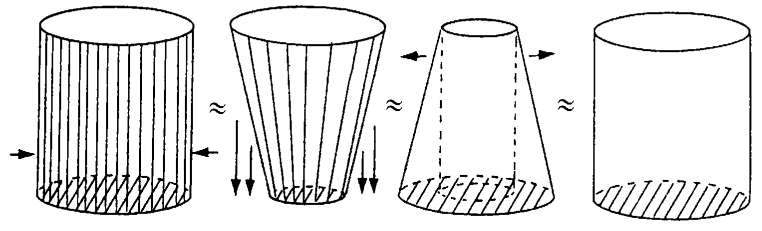
\includegraphics[width=0.8\textwidth]{Figures/DUWUWUJK122.png}
        \caption{A homeomorphism of pairs.}
        \label{fig:DUWUWUJK122-png}
    \end{figure}
    These maps for each cell fit together to
    give a map on the $r$-skeleton because of the
    weak topology on $X \times I$. The union of these
    maps for all $r$ gives a map on $X \times I$, again because
    of the weak topology on $X \times I$.
\end{proof}

\begin{theorem}[]\label{Thm:SJJDHW29WW}
    Assume that $A \subset X$ is closed and that there
    exists a neighborhood $U$ of $A$ and a map
    $\varphi  \colon X \to I$ such that
    \begin{enumerate}
        \item $A = \varphi ^{-1} (0)$.
        \item $\varphi \left( X-U \right) = \left\{ 1 \right\} $.
        \item $U$ deforms to $A$ through $X$ with $A$ fixed.
            That is, there is a map $H \colon U \times I \to X$ 
            such that $H(a,t) = a$ for all $a \in A, H
            (u,0) = 0$, and $H(u,1) \in A$ for all $u \in U$.
    \end{enumerate}
    Then the inclusion
    $A \hookrightarrow X$ is a cofibration. The converse also
    holds.
\end{theorem}

\begin{proof}
    We may assume that $\varphi  = 1$ on a neighborhood
    of $X - U$ by replacing $\varphi $ with
    $\min \left( 2 \varphi , 1 \right) $.
    It suffices to show that there exists a retract
    $\Phi \colon U \times I \to X \times \left\{ 0 \right\} 
    \cup A \times I$ since then the
    map
    \[
    r\left( x,t \right) 
    =
    \begin{cases}
        \Phi\left( x, t \left( 1-\varphi (x) \right)  \right),&
        x \in U\\
        (x,0),& x \not\in U
    \end{cases}
    \] 
    gives a retraction $X \times I \to A \times I \cup 
    X \times \left\{ 0 \right\} $.\\
    We define $\Phi$ by
    \[
    \Phi(u,t) = 
    \begin{cases}
        H\left( u, \frac{t}{\varphi (u)} \right) \times 
        \left\{ 0 \right\},& \varphi (u) > t\\
        H\left( u,1 \right) \times 
        \left\{ t- \varphi (u) \right\} ,& \varphi (u)\le t.
    \end{cases}
    \] 
    The only thing that needs checking here is
    that $\Phi$ is continuous at
    points $\left( u,0 \right) $ such that
    $\varphi (u) = 0$, i.e., points $(a,0)$ for 
    $a \in A$ - indeed here the expression for
    $\varphi (u) > t$ is not defined.

    Recall that a map $f \colon X \to Y$ is continuous
    if for every point $x \in X$ and any neighborhood
    $U$ of $f(x)$, there exists a neighborhood
    $V$ of $x$ such that $f(V) \subset U$.\\
    So let $W$ be a neighborhood of $a = 
    H(a,t)$. Then there exists a neighborhood
    $V \subset W$ containing $a$ such that
    $H\left( V \times I \right) \subset W$, by
    assumption of $H$ being continuous.
    So for $t < \varepsilon$ for some $\varepsilon$ and
    $u \in V$, we have
    $\Phi \left( u,t \right) 
    \in W \times \left[ 0,\varepsilon \right] $.
    Hence $\Phi$ is continuous.\\
    \linebreak
    To prove the converse, suppose that the
    inclusion $A \hookrightarrow X$ is a cofibration. Equivalently,
    $A \times I \cup  X \times \left\{ 0 \right\} $ is
    a retract of $X \times I$. Let $r
    \colon X \times I \to  A \times I \cup X \times
    \left\{ 0 \right\} $ be this retraction.
    Let $s(x) = r\left( x,1 \right) $ and set
    $U = s^{-1}\left( A \times (0,1] \right) $.
    Let $p_X, p_I$ be the projections of
    $X \times I$ to its factors. Then
    put $H = p_X \circ r|_{U \times I} \colon U \times I \to X$.
    Now, $H(a,t) = p_X \circ r |_{U \times I}(a,t)
    = p_X \left( a,t \right) = a$ for all
    $a \in A$ and $t \in I$;
    $H(u,0) = p_X \circ r|_{U \times I}(u,0) =
    p_X \left( u,0 \right) = u$, and
    $H\left( u,1 \right) =
    p_X \circ r|_{U \times I}(u,1) = 
    u$ forces $(u,1) \in A \times I$, hence
    $u \in A$. Thus, $H$ satisfies condition (3).\\
    For (1) and (2), let
    $\varphi (x) = 
    \max_{t \in I} \left| t - p_I r(x,t) \right| $ which
    is possible since $I$ is compact. Then
    $x \in \varphi^{-1}(0)$ implies that
    $\max_{t \in I} \left| t - p_I r(x,t) \right| = 0$, so
    for all $t \in I$, we have
    $\left| t - p_I r(x,t) \right| = 0$, so
    $r(x,t) \in A \times \left\{ t \right\} $ for all
    $t \in (0,1]$. Then
    $r\left( x,0 \right) = \lim_{n \to \infty}
    r\left( x, \frac{1}{n} \right) 
    \in A \times I$ since $A \times I$ is closed. But
    $(x,0) = r(x,0)$, so $x \in A$. Conversely, for any
    $x \in A$, clearly, $\varphi (x) = 0$ since
    $r(x,t) = (x,t)$ for all $t \in I$. This shows that
    $\varphi $ satisfies (1). 
    For (2), we have that for
    $x \in X -U$, with $U = 
    s^{-1}\left( A \times (0,1] \right) $, we
    have $r(x,1) = s(x) \not\in A \times (0,1]$, so
    $r(x,1) \in X \times \left\{ 0 \right\} $. Hence
    $\varphi (x) = 
    \max_{t \in I} \left| t - p_I r(x,t) \right| = 1$, giving
    (2).\\
    It remains to show that $\varphi $ is continuous.
    Let $f(x,t) = \left| t - p_I r(x,t) \right| $ and
    $f_t = (x,t)$ all of which are continuous.
    Then
    \[
        \varphi^{-1} \left( (- \infty, b] \right) 
        = \left\{ x  \mid f(x,t) \le b \text{ for all }t 
        \right\} = 
        \bigcap_{i \in  I} f_t^{-1}\left( (- \infty, b] \right) .
    \]
    is an intersection of closed sets and so is closed.
    Similarly,
    \[
    \varphi^{-1} \left( [a, \infty) \right) 
    = \left\{ x  \mid  f(x,t) \ge a \text{ for some }t \right\} 
    = p_X \left( f^{-1} \left( [a, \infty) \right)  \right) 
    \] 
    which si also closed since $p_X$ is closed as
    a projection and
    $I$ is compact.
    Since the complements of the intervals of the
    form $[a, \infty)$ and 
    $(-\infty, b]$ give a subbase for the topology of
    $\mathbb{R}$, this shows that
    $\varphi $ is continuous.





\end{proof}


Next, we recall that for a map
$f \colon X \to Y$, the mapping cylinder
$M_f$ is defined as
\[
M_f = \left( \left( X \times I \right) \sqcup Y \right) 
/ \left( \left( x,0 \right) \sim f(x) \right) .
\] 
Consider the inclusion
$\iota \colon X \hookrightarrow 
M_f$ where we include $X$ as
$X \times \left\{ 1 \right\} $.
Consider the map
$ \varphi \colon
M f \to I$ given by
$ \varphi (x,t)  =  1 - 2t$ for
$t \ge \frac{1}{2}$ and
$\varphi (x,t) = 1$ on the rest of $M_f$. Choosing
$U = X \times (\frac{1}{3}, 1]$, $U$ clearly
deformations retracts to $X \times \left\{ 1 \right\} $ and
satisfies the conditions of 
Theorem \ref{Thm:SJJDHW29WW}, hence
the inclusion $X \hookrightarrow M_f$ is a cofibration.
Also, the retraction
$r \colon M_f \to Y$ is a homotopy equivalence
with the homotopy inverse being the inclusion
$Y \hookrightarrow M_f$. The diagram
\begin{equation*}
\begin{tikzcd}
    X \ar[rr, "\iota"] \ar[ddr, "f"'] & & M_f \ar[ddl, "r", "\simeq"']\\ 
                                     &&\\
                                     & Y &
\end{tikzcd}
\end{equation*}
commutes.
Thus any map $f$ is a cofibration up to
a homotopy equivalence of spaces.

Recall also that the mapping cone of a
map $f \colon X \to Y$ is defined as
\[
C_f := M_f / X \times \left\{ 1 \right\} 
\cong M_f \cup CX.
\] 
In the case of an inclusion
$\iota \colon A \hookrightarrow X$, we have
$C_{\iota} = X \cup  CA$.\\
There is a map
$C_{\iota} \stackrel{h}{\to} X / A$, defined
as the composite of the quotient map
$X \cup  CA \to X \cup  CA /CA$ composed with the
inverse of the homeomorphism $X / A \to 
X \cup  CA /CA$.

\begin{question}
    Is $h$ a homotopy equivalence?
\end{question}

\begin{theorem}[]\label{Thm:2030akKAK}
    If $A \subset X$ is closed and the inclusion
    $\iota \colon A \to X$ is a cofibration, then
    $h \colon C_{\iota} \to X /A$ is a homotopy equivalence.
    In fact, it is a homotopy equivalence of pairs
    \[
        \left( X /A, * \right) \simeq
        \left( C_{\iota}, CA \right) \simeq
        \left( C_{\iota}, v \right) ,
    \] 
    where $v$ is the vertex of the cone.
\end{theorem}

\begin{proof}
    The mapping cone $C_{\iota} = X
    \cup CA$ consists of three different types of
    points: the vertex $v = \left\{ A \times \left\{ 1 \right\} 
    \right\} $, the rest of the cone
    $\left\{ \left( a,t \right)  \mid 0\le t < 1 \right\} $ 
    where $\left( a,0 \right) = a \in A \subset X$, and
    points in $X$ itself, which we identify with $X \times 
    \left\{ 0 \right\} $.\\
    Define $f \colon A \times I \cup  X \times \left\{ 0 \right\} 
    \to C_{\iota}$ as the collapsing map and extend
    $f$ to $\overline{f} \colon X \times I \to 
    C_{\iota}$ using that $f$ is a cofibration. 
    Then $\overline{f}\left( a,1 \right) =
    v, \overline{f}(a,t) = (a,t)$ and
    $\overline{f}(x,0) = x$.\\
    Let $\overline{f}_t = 
    \overline{f}|_{X \times \left\{ t \right\} }$.
    Since $\overline{f}_1 (A) = \left\{ v \right\} $, 
    we can factorize $\overline{f}_1 \colon
    X \to C_{\iota}$ as
    $g \circ j$ where
    $j \colon X \to X /A$ is the quotient map
    and $g \colon X / A \to C_{\iota}$ is
    the induced map
    \begin{equation*}
    \begin{tikzcd}
        X \ar[d, "j"] \ar[dr, "\overline{f}_1"] & \\
        X / A \ar[r, "g", dashed] & C_{\iota}.
    \end{tikzcd}
    \end{equation*}
    where $g$ is induced and continuous by
    definition of the quotient topology.\\
    We claim that $g$ is a homotopy equivalence with
    homotopy inverse $h$.
    First, we prove that $hg \simeq \id_{X / A}$.

    Note that taking the composite
    $h \overline{f}_t \colon X \to X / A$ gives a homotopy
    between $h \overline{f}_0$ and $h \overline{f}_1$.
    For all $t$, this homotopy takes
    $A$ to the point $\left\{ A \right\} $. Thus, it
    factors to give a homotopy
    \[
    hgj = h \overline{f}_1 
    \simeq h \overline{f}_0 = j
    \] 
    Let $H \colon X \times I \to X / A$ be the homotopy
    between $hgj$ and $j$, so
    $H(x, 0) = hgj(x)$ and
    $H(x,1) = j(x)$. Then
    the map
    $\overline{H} \colon X / A \times I \to X / A$ defined
    by
    $\overline{H}(\left[ x \right] ,t) = 
    H\left( x,t \right) $ defines a homotopy
    between $hg$ and $\id_{X / A}$, so
    $hg \simeq \id_{X / A}$.

    Next, we will show that $gh \simeq \id_{C_{\iota}}$.
    Consider $W = \left( X \times I \right) / 
    \left( A \times \left\{ 1 \right\}  \right) $ 
    and the maps illustrated in Figure \ref{fig:DWIJJXNXJNXJUI-png}.

    \begin{figure}[htpb]
        \centering
        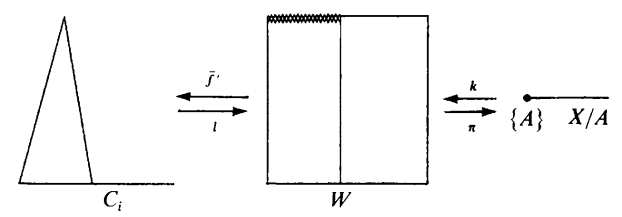
\includegraphics[width=0.8\textwidth]{Figures/DWIJJXNXJNXJUI.png}
        \caption{}
        \label{fig:DWIJJXNXJNXJUI-png}
    \end{figure}
    The map $\overline{f}'$ is induced by
    $\overline{f}$. The map
    $k$ is the "top face" map.
    From this, we see that
    \begin{align*}
        \overline{f}' \circ l 
        &= \id \\
        \pi \circ k 
        &= \id \\
        k \circ \pi 
        &\simeq \id \\
        \overline{f}' \circ k
        &= g \\
        \pi \circ l 
        &= l.
    \end{align*}
   Hence $g h = \overline{f}' k \pi l 
   \simeq \overline{f}' l = \id$. 
\end{proof}


\begin{example}[A non example]
    An example of when the result
    of Theorem 1.6 does not hold is with
    $A = \left\{ 0 \right\} \cup 
    \left\{ \frac{1}{n} \mid n = 1, 2, \ldots \right\} $ 
    and $X = \left[ 0,1 \right] $.
    In this case, $C_{\iota}$ is not homotopy equivalent
    to $X / A$ which is a one-point union of a countably infinite
    sequence of circles with radii going to zero.

    $C_i$ has homeomorphs of circles joined along edges. However,
    the circles do not tend to a point ,so any prospective homotopy
    equivalence $X / A \to C_{\iota}$ would be discontinuous at
    the image of $\left\{ 0 \right\} $ in $X / A$.
\end{example}

\begin{corollary}\label{Cor:Cofibration-Homology}
    If $A \subset X$ is closed and the inclusion
    $A \hookrightarrow X$ is a cofibration, then the map
    $j \colon \left( X, A \right) \to 
    \left( X / A, * \right) $ induces isomorphisms
    \[
    H_* (X,A) \stackrel{\cong}{\to} 
    H_* \left( X / A, * \right) 
    \cong \tilde{H}_* \left( X / A \right) 
    \] 
    and
    \[
    \tilde{H}^{*}(X /A) \cong
    H^{*} (X / A, *) 
    \stackrel{\cong}{\to} H^{*} (X , A).
    \] 
\end{corollary}

\begin{proof}
    We have
    $H_* \left( X/A , *\right) \cong
    H_* \left( C_{\iota}, CA \right) $ by Theorem
    \ref{Thm:2030akKAK}. And since
    $C_{\iota} = X \cup A \times \left[ 0,\frac{1}{2} \right] $ 
    and $CA = A \times \left[ 0,\frac{1}{2} \right] $, where
    we collapse $A \times \left\{ \frac{1}{2} \right\} $ in
    both, and attach  $A \times \left[ 0,\frac{1}{2} \right] $ 
    along $A \times \left\{ 0 \right\} $ in
    $X \cup A \times \left[ 0,\frac{1}{2} \right] $, we obtain
    \[
    H_*(C_{\iota}, CA) \cong
    H_* \left( X \cup A \times \left[ 0,\frac{1}{2} \right] ,
    A \times \left[ 0, \frac{1}{2} \right] \right) 
    \cong H_* (X, A)
    \] 
    since 
    $\left( X \cup A \times \left[ 0,\frac{1}{2} \right] ,
    A \times \left[ 0,\frac{1}{2} \right] \right) 
    \simeq \left( X,A \right) $ by deformation retracting
    $A \times \left[ 0,\frac{1}{2} \right] $ down to
    $A \times \left\{ 0 \right\} \subset X$.
\end{proof}


\subsubsection{Interlude on pointed-spaces and
operations on spaces}

We recall some important constructions:

\begin{definition}[Unreduced Suspension]
    For a space $X$, the \textit{unreduced suspension} 
    $\Sigma X$ is the
    quotient obtained from $X \times I$ by
    collapsing $X \times \left\{ 0 \right\} $ to one
    point and $X \times \left\{ 1 \right\} $ to another
    point.
\end{definition}

\begin{note}
    We have $\Sigma S^{n} = S^{n+1}$.
\end{note}



\begin{definition}[Suspension of a map]
    Given a map
    $f \colon X \to Y$, we can suspend $f$ to
    $\Sigma f \colon \Sigma X \to \Sigma Y$
    by letting $\Sigma f$ be the induced
    map on the quotients:
    \begin{equation*}
    \begin{tikzcd}
        X \times I \ar[r, "f \times \id"] \ar[d]  & Y \times I \ar[d] \\
        \Sigma X \ar[r, "\Sigma f"] & \Sigma Y
    \end{tikzcd}
    \end{equation*}
    
\end{definition}

\begin{definition}[Reduced Suspension]
    For a space $X$, the \textit{reduced suspension}
    $SX$ is the quotient
    \[
    SX = X \times I / \left( X \times \partial I
    \cup \left\{ * \right\} \times I \right) .
    \] 
\end{definition}

\begin{definition}[Reduced Suspension of a map]
    The reduced suspension of a map $f \colon X \to Y$ is
    the induced map on the reduced suspensions of
    $X$ and $Y$ :
    \begin{equation*}
    \begin{tikzcd}
        X \times I \ar[r, "f \times \id"]
        \ar[d] & Y \times I \ar[d] \\
        SX \ar[r, "Sf"] & SY
    \end{tikzcd}
    \end{equation*}
    
\end{definition}

\begin{exercise}[]
    For any homology theory, show that
    there is a natural isomorphism
    $\tilde{H}_I (X) \stackrel{\cong}{\to} 
    \tilde{H}_{i+1} \left( \Sigma X \right) $. Here,
    natural means that for a map $f \colon X \to Y$,
    and its suspension $\Sigma f \colon \Sigma X \to 
    \Sigma Y$, the following diagram commutes:
    \begin{equation*}
    \begin{tikzcd}
        \tilde{H}_i (X) \ar[r, "\cong"] \ar[d, "f_*"]& 
        \tilde{H}_{i+1} \left( \Sigma X \right)
        \ar[d, "(\Sigma f)_*"] \\
        \tilde{H}_i (Y) \ar[r, "\cong"] & \tilde{H}_{i+1}
        \left( \Sigma Y \right) 
    \end{tikzcd}
    \end{equation*}
    
\end{exercise}


\begin{definition}[Wedge Sum/one-point union]
    Given two pointed spaces $(X, x_0), \left( Y, y_0 \right) $,
    we define
    the \textit{wedge sum}  $X \vee Y$ to be
    \[
    X \vee Y = X \sqcup Y / \left( x_0 \sim y_0 \right) ,
    \] 
    i.e., the quotient of the disjoint union identifying
    $x_0$ and $y_0$ to a single point.
\end{definition}

\begin{definition}[Smash Product]
    Inside the product $X \times Y$
    of two pointed space $(X,x_0), (Y,y_0)$,
    we have natural copies of $X$ and $Y$ by
    $X \times \left\{ y_0 \right\} $ and
    $\left\{ x_0 \right\} \times Y$, respectively.
    These two copies intersect only at the point
    $\left( x_0,y_0 \right) $, so their union can
    be identified with
    the wedge sum $X \vee Y$. I.e., $X \vee Y = 
    X \times \left\{ y_0 \right\} \cup 
    \left\{ x_0 \right\} \times Y$. We define
    the \textit{smash product} $X \wedge Y$ to be
    the quotient $X \times Y / X \vee Y$.
\end{definition}


If $f \colon X \to Y$ is a pointed map, then
the reduced mapping cylinder of $f$ is defined
as the quotient space $M_f$ of
$\left( X \times I \right) \cup  Y$ modulo the relations
identifying
$\left( x,0 \right) \sim f(x)$ and the set
$\left\{ * \right\} \times I$ to the base point of $M_f$.\\
The reduced mapping cone is the quotient of the reduced
mapping cylinder $M_f$ obtained by identifying the image of
$X \times \left\{ 1 \right\} $ to a point, the
base point.\\

The circle $S^{1}$ is defined as
$I / \partial I$ with base point $\left\{ \partial I \right\} $.\\
The reduced suspension of a pointed space $X$ is
$SX = X \wedge S^{1}$. It can also be considered
as the quotient space $X \times I / \left( X \times 
\partial I \cup  \left\{ * \right\} \times I\right) $


\begin{definition}[Well-pointed space]
    A base point $x_0 \in X$ is said to be
    \textit{nondegenerate} if the inclusion
    $\left\{ x_0 \right\} \hookrightarrow X$ is a cofibration.
    A pointed Hausdorff space $X$ with nondegenerate
    base point is said to be \textit{well-pointed}.
\end{definition}

It is clear that any manifold or CW-complex satisfies
Theorem \ref{Thm:SJJDHW29WW} with $A$ being any point of
the space. Hence any manifold or CW-complex is
well-pointed.\\

\begin{example}[Pointed space that is not well-pointed]
    Taking the pointed space  $X = 
    \left\{ 0 \right\} \cup  \left\{ \frac{1}{n} \mid 
    n \in \mathbb{N} \right\} $ with base point $0$, this
    space is not well-pointed. This can for example be
    seen because it fails to satisfy Theorem
    \ref{Thm:Retract-cofibration} - any retraction
    would break continuity at
    $\left( 0,1 \right) $.
\end{example}

\begin{example}[]
    If $A \hookrightarrow X$ is a cofibration, then
    $X / A$ with base point $\left\{ A \right\} $ is well-pointed,
    as follows from Theorem \ref{Thm:SJJDHW29WW}.
\end{example}

\begin{theorem}[]
    If $X$ is well-pointed, then so are the reduced
    cone $CX$ and the reduced suspension $SX$. Moreover,
    the collapsing map  $\Sigma X \to SX$, of the unreduced
    suspension to the reduced suspension, is a homotopy
    equivalence.
\end{theorem}

\begin{proof}
    Denote the base point of $X$ by $*$.
    Consider the homeomorphism
    \[
    h \colon \left( I \times I,
    I \times \left\{ 0 \right\} \cup 
\partial I \times I \right) 
\stackrel{\cong}{\to} \left( I \times I, I \times 
\left\{ 0 \right\} \right) 
    \] 
    which clearly exists. For example, take Figure
    \ref{fig:IWIDK01-jpeg}
    \begin{figure}[htpb]
        \centering
        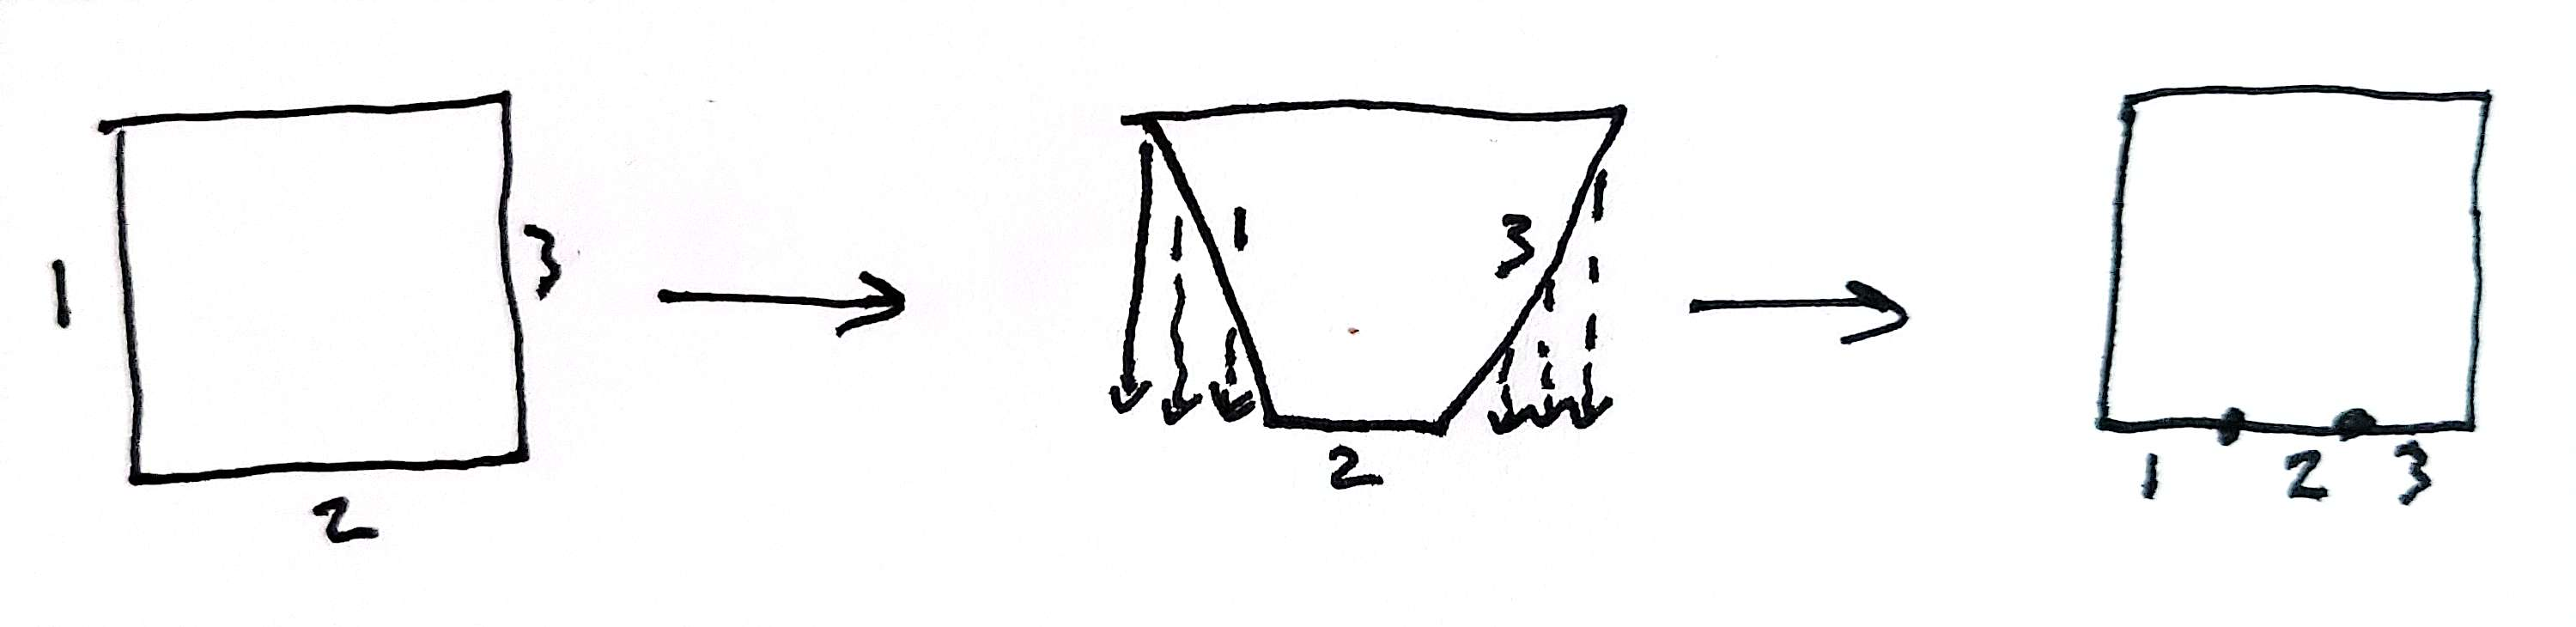
\includegraphics[width=0.5\textwidth]{Figures/IWIDK01.jpeg}
        \caption{}
        \label{fig:IWIDK01-jpeg}
    \end{figure}

    Then the induced homeomorphism
    \[
    \id_X \times h\colon X \times I \times I 
    \stackrel{\cong}{\to} X \times I \times I
    \] 
    carries 
    $X \times I \times \left\{ 0 \right\} \cup 
    X \times \partial I\times I$ to
    $X \times I \times \left\{ 0 \right\} $.
    Hence it takes
    $A = X \times I \times \left\{ 0 \right\} \cup 
    X \times \partial I \times I \cup 
    \left\{ * \right\} \times I \times I$ to
    $X \times I \times \left\{ 0 \right\} 
    \cup \left\{ * \right\} \times I \times I$. 
    Therefore, the pair
    $\left( X \times I \times I, A \right) $ is homeomorphic
    to the pair
    $I \times \left( X \times I, 
    X \times \left\{ 0 \right\} \cup 
\left\{ * \right\} \times I \right) $.
Now, $X$ is well-pointed, so
$X \times \left\{ 0 \right\} \cup 
\left\{ * \right\} \times I$ is a retract of
$X \times I$ by
Theorem \ref{Thm:Retract-cofibration} and the
definition of well-pointed.
It follows that
$A$ is a retract of
$X \times I \times I$.
By another application of
\ref{Thm:Retract-cofibration}, then
the inclusion
$X \times \partial I \cup \left\{ * \right\} \times I
\hookrightarrow X \times I$ is a cofibration. 
Hence the quotient by this,
$SX = X \times I / \left( X \times \partial I
\cup \left\{ * \right\} \times I \right) $ is well-pointed,
using the quotient of the above inclusion.\\
\linebreak
Next consider the homeomorphism
$\left( I \times I, I \times \left\{ 0 \right\} \cup 
\left\{ 1 \right\} \times I \right) 
\stackrel{\cong}{\to} \left( 
I \times I, I \times \left\{ 0 \right\} \right) $ which
can be seen similarly. The induced
homeomorphism
\[
1 \times h \colon X \times I \times I
\stackrel{\cong}{\to} X \times I \times I
\] 
takes
$A:= X \times \left\{ 1 \right\} \times I \cup 
\left\{ * \right\} \times I \times I
\cup X \times I \times \left\{ 0 \right\} $ to
$X \times I \times \left\{ 0 \right\} \cup 
\left\{ * \right\} \times I \times I$.
Thus the pair
$\left( X \times I \times I,
A\right) $ is homeomorphic to
 $I \times \left( X \times I,
 X \times \left\{ 0 \right\} \cup 
\left\{ * \right\} \times I\right) $.
Just as above, we have that
$X \times \left\{ 0 \right\} \cup 
\left\{ * \right\} \times I$ is a retract
of $X \times I$, so
it follows that
$A$ is a retract of $X \times I \times I$. Thus
the inclusion
$X \times \left\{ 1 \right\} \cup 
\left\{ * \right\} \times I \hookrightarrow
X \times I$ is a cofibration, which shows
that $CX = X \times I / \left( X \times \left\{ 1 \right\} 
\cup \left\{ * \right\} \times I\right) $ is
well-pointed.\\
\linebreak
The fact that
$X \times \partial I \cup \left\{ * \right\} \times I
\hookrightarrow X \times I$ is a cofibration
gives that there exists a neighborhood $U$ of
$X \times \partial I \cup 
\left\{ * \right\} \times I$ and a map
$\varphi \colon X \times I \to I$ 
that satisfy Theorem \ref{Thm:SJJDHW29WW}.
We obtain an induced map
$\overline{\varphi }\colon
\Sigma X \to I$ 
which satisfies the same conditions, so
$I \times \times \left\{ * \right\} \times I
\hookrightarrow X \times I / 
\left\{ X \times \left\{ 0 \right\} ,
X \times \left\{ 1 \right\} \right\} = \Sigma X$ is a
cofibration. Now 
Theorem \ref{Thm:2030akKAK} implies
that $\Sigma X \cup CI = C_{\iota} \to \Sigma X / I$ is a homotopy
equivalence.
Hence we obtain
that 
$\Sigma X \simeq
\Sigma X \cup CI \simeq
\Sigma X / I = SX$, via the collapsing map.

\end{proof}


\begin{problem}[]
    Find $H_* \left( \mathbb{P}^2, \mathbb{P}^{1} \right) $ 
    using methods or results from this section.
\end{problem}

\begin{solution}
    Consider $\mathbb{P}^2$ as 
    $S^2$ quotiented by the relation
    $x \simeq -x$. Then
    we can think of  $\mathbb{P}^{1}$ as
    $S^{1} \subset S^{2}$ under this relation.
    We want to show that the inclusion
    $\mathbb{P}^{1} \hookrightarrow \mathbb{P}^2$ is a
    cofibration. 
    Using Theorem \ref{Thm:SJJDHW29WW}, it suffices to
    find a neighborhood $U$ of $\mathbb{P}^{1} \subset 
    \mathbb{P}^2$ and a map $\overline{\varphi } \colon
    \mathbb{P}^2 \to I$ such that
    the conditions of the theorem are satisfied.
    We construct a preliminary map on
    $S^2$ towards this end. 
    Define $\varphi \colon S^2 \to I$ to be
    $\varphi (x) = 
    \min \left\{ 1, 2 \left| x_3 \right|  \right\} $, where
    $x_3$ is the last coordinate of $x$. Since
    $\varphi (x) = \varphi (-x)$, $\varphi $ induces
    a map $\overline{\varphi }\colon
    \mathbb{P}^2 \to I$ such that the diagram
    \begin{equation*}
    \begin{tikzcd}
        S^2 \ar[d] \ar[dr, "\varphi "] & \\
        \mathbb{P}^2 \ar[r, "\overline{\varphi }"] & I
    \end{tikzcd}
    \end{equation*}
    commutes.
    Letting $U$ be the image under the quotient
    map of 
    $\left\{ x \in S^2  \mid 
    \left| x_3 \right| < \frac{1}{2} \right\} $, this
    becomes an open set in $\mathbb{P}^2$ since 
    the above set is saturated with respect to the quotient
    map. It is also clear that
    $U$ and $\overline{\varphi }$ satisfy the conditions of
    the theorem, hence the inclusion
    $\mathbb{P}^{1} \hookrightarrow \mathbb{P}^2$ is a cofibration.
    By Corollary \ref{Cor:Cofibration-Homology}, we
    obtain that
    $H_* \left( \mathbb{P}^2, \mathbb{P}^{1} \right) 
    \cong \tilde{H}_* \left( \mathbb{P}^2 / \mathbb{P}^{1} \right) $.
    But $\mathbb{P}^2 / \mathbb{P}^{1} \cong
    S^{2}$, so
    $H_* \left( \mathbb{P}^2, \mathbb{P}^{1} \right) 
    \cong \tilde{H}_* \left( S^2 \right)$.
    Now simply recall that
    \[
    \tilde{H}_p \left( S^2 \right) 
    \cong
    \begin{cases}
        \mathbb{Z},& p = 2\\
        0,& p \neq 2.
    \end{cases}
    \] 
    \qed
\end{solution}

\begin{problem}[]
    Find $H_*\left( T^2,
    \left\{ * \right\} \times S^{1} \cup 
S^{1} \times \left\{ * \right\} \right) $ using
methods from this section.
\end{problem}

\begin{solution}
    If we can show that the inclusion
    $A:= \left\{ * \right\} \times S^{1} \cup 
    S^{1} \times \left\{ * \right\} \hookrightarrow
    T^2$ is a cofibration, then
    we will again obtain that
    $H_* (T^2, A) \cong
    \tilde{H}_* \left( T^2 / A \right) \cong
    \tilde{H}_* \left( S^2 \right) $.
    But we have a CW-structure on the
    torus given by the square with identified sides.
    With this identificaiton, $A$ simple becomes
    the $1$-skeleton, hence it is a subcomplex, so
    by Corollary \ref{Cor:Subcomplex-Cofibration}, 
    the inclusion $A \hookrightarrow T^2$ is a cofibration.
    This finishes the solution. \qed
\end{solution}

\begin{problem}[]
    For a space $X$, consider the pair
    $\left( CX, X \right) $. What do the results of this
    section tell you about the homology of these, and related,
    spaces?
\end{problem}


\begin{solution}
    We can define a map
    $\varphi \colon CX \to I$ by
    $\varphi (x,t) = t$. Choosing
    $A = X = X \times \left\{ 0 \right\} \subset 
    CX$ and
    $U = CX - \left\{ v \right\} $ where
    $v$ is the vertex, this satisfies the
    conditions in Theorem \ref{Thm:SJJDHW29WW} 
    ($H$ can be defined by
    $H((x,t_0),t) = \left( x,t_0 \right) (1-t)
    + (x,0) t$).
    Hence the inclusion
    $X \hookrightarrow CX$ is a cofibration, so we
    know that
    $H_* \left( CX, X \right) 
    \cong \tilde{H}_* \left( CX / X \right) $.
    Similarly, one can
    show that the inclusion
    $X \hookrightarrow \Sigma X$ is a cofibration, so
    $H_* \left( \Sigma X , X \right) 
    \cong \tilde{H}_* \left( \Sigma X / X \right) 
    \cong \tilde{H}_* \left( 
    \Sigma X \vee \Sigma X \right) $ and
    $H_*\left( SX, X \right) 
    \cong \tilde{H}_* \left( SX \vee SX \right) $.
\end{solution}


\begin{problem}[]
    If $f \colon A \to X$ is a cofibration then show that
    $f$ is an embedding. If $X$ is also Hausdorff,
    then show that $f(A)$ is closed in $X$.
\end{problem}

\begin{proof}
    Since $f$ is a cofibration, the following diagram
    can be filled out, inducing a map
    $g \colon X \times I \to M_f$ :
    \begin{equation*}
    \begin{tikzcd}
        A \times \left\{ 0 \right\} \ar[dd, "f \times \id"] 
        \ar[rr, hookrightarrow] & & A \times I \ar[dd, "f \times 
        \id"] \ar[dl, "q"] \\
                                & M_f & \\
        X \times \left\{ 0 \right\} \ar[ur, "q"] 
        \ar[rr, hookrightarrow]& & X \times I 
        \ar[ul, "g"]
    \end{tikzcd}
    \end{equation*}
    By construction, we have that
    $q \colon A \times \left\{ 1 \right\} 
    \hookrightarrow M_f$ is an embedding, so
    letting $l \colon
    q \left( A \times \left\{ 1 \right\}  \right) 
    \to A \times \left\{ 1 \right\} $ be the inverse map,
    we have
    $l \circ g|_{f(A) \times \left\{ 1 \right\} } 
    \circ \left( f \times \id \right) 
    = \id_{A \times \left\{ 1 \right\} }$.
    Likewise,
    $\left( f \times \id \right) 
    \circ l \circ g|_{f(A) \times \left\{ 1 \right\} }$,
    since $g \left( f(a), t \right) 
    = q(a,t)$, we have that
    $l \circ g|_{f(A) \times \left\{ 1 \right\} }
    (f(a),1) = (a,t)$, hence
    $\left( f \times \id \right) 
    \circ l \circ g|_{f(A) \times \left\{ 1 \right\} }
    = \id_{f(A) \times \left\{ 1 \right\} }$.
    Therefore,
    $f \times \id$ is a homeomorphism
    $A \times \left\{ 1 \right\}  \stackrel{\cong}{\to} 
    f(A) \times \left\{ 1 \right\} $, so
    $f \colon A \stackrel{\cong}{\to} f(A)$ is a homeomorphism.\\
    \linebreak
    By Lemma \ref{Lemma:Cofibration-Inclusion-2} and
    Theorem \ref{Thm:Retract-cofibration}, we
    have that there exists a retraction
    $r \colon X \times I \to 
    X \times \left\{ 0 \right\} \cup 
    f(A) \times I$.

    \begin{lemma}[]
         If a space $X$ is Hausdorff and
          there exists a retraction
          $r \colon X \to A$, then $A$ is closed.
    \end{lemma}

    \begin{proof}
        Let
        $x \in X -A$ be a limit point of $A$. Let
        $U ,V$ be open disjoint neighborhoods of
        $x$ and $r(x)$. Then
        $r^{-1}(V)$ is open and contains $x$, so
        let $U' = U \cap r^{-1}(V)$.
        Now $U \cap A \cap r^{-1}(V) = \varnothing$ since
        otherwise $U \cap A = r\left( U \cap A \right) 
        \subset V$ contradicting $U \cap V = \varnothing$.
        But then $U'$ is an open neighborhood of $x$
        that is disjoint from $A$, contradicting $x$ being
        a limit point of $A$.
        Thus $\overline{A} = A$.
    \end{proof}

    Using this Lemma, we find that since
    $X \times I$ is Hausdorff and
    $r \colon X \times I \to X \times \left\{ 0 \right\} 
    \cup f(A) \times I$ is a retraction,
    $X \times \left\{ 0 \right\} \cup 
    f(A) \times I$ is closed in
    $X \times I$.
    Now,
    $f(A) \times \left\{ 1 \right\} 
    = X \times \left\{ 1 \right\} 
    \cap \left( X \times \left\{ 0 \right\} \cup 
    f(A) \times I\right) $, so
    since $X \times \left\{ 1 \right\} $ is closed
    in $X \times I$,
    $f(A) \times \left\{ 1 \right\} $ 
    is by definition closed in 
    $X \times \left\{ 0 \right\} \cup 
    f(A) \times I$ in the subspace topology. Hence
    it is also closed in $X \times I$.
    Now we use another lemma:
    \begin{lemma}[]
        If $Y$ is a compact space, then
        the projection $X \times Y \to X$ is a closed map.
    \end{lemma}
    \begin{proof}
        Let $W \subset X \times Y$ be closed and
        set $W' = X \times Y -W$.
        Note that $x_0 \in \pi_X (W)$ if and only
        if $\exists y_0 \in Y$ such that
        $(x_0,y_0) \in W$. Thus
        $x_0 \not\in \pi_X(W)$ if and only if
        $\left\{ x_0 \right\} \times Y \subset 
        W'$.

        By the tube lemma,
        $x_0 \not\in \pi_X (W)$ if and only if
        $W'$ contains some tube
        $N \times Y$ about $\left\{ x_0 \right\} \times Y$ 
        where $N$ is an open neighborhood of $x_0$ in $X$. 
        But then
        $N = \pi(N \times Y) \subset 
        X - \pi(W)$ is an open neighborhood of $x_0$ in
        $X - \pi(W)$. Hence
        $X - \pi(W)$ is open, so $\pi(W)$ is
        closed.
    \end{proof}
    Noting that
    $\left\{ 1 \right\} \subset I$ is compact,
    we can apply this Lemma to
    $f(A) \times \left\{ 1 \right\} $ to obtain that
    $f(A)$ is closed in $X$.
    This completes the proof.

\end{proof}

\newpage
\begin{problem}[]
    Let $\iota \colon A \hookrightarrow X$,
    the inclusion of $A$ in $X$, be a cofibration and
    $A$ be a contractible space. Show that the
    quotient map $X \to X / A$ is a homotopy equivalence.
\end{problem}

\begin{proof}
    Let
    $H \colon A \times I \to A$ be the contraction of
    $A$ where
    $H(a,0) = a$ and $H(a,1) = a_0 \in A$.
    Consider the diagram
    \begin{equation*}
    \begin{tikzcd}
        A \times \left\{ 0 \right\} \ar[dd, "\iota \times \id"]
        \ar[rr] 
        & &
        A \times I \ar[dd, "\iota \times \id"] \ar[dl, "H"] \\
                                                    & X&\\
        X \times \left\{ 0 \right\} \ar[rr] \ar[ru,"\id"]
                                                    & & X \times I
        \ar[ul, "\tilde{H}"] 
    \end{tikzcd}
    \end{equation*}
    Then since 
    $\tilde{H}(a,t) \in A$ for all $t$,
    the composition $q \tilde{H} \colon X \times I \to X / A$ sends
    $A$ to a point at all times, hence factors as
    $X \times I \stackrel{q \times \id}{\to} X / A \times I
    \to X / A$. Denote the
    latter map by $\overline{H} \colon 
    X / A \times I \to X / A$. Then
    $q \tilde{H} = \overline{H} \left( q \times \id \right) $.
    When $t = 1$, we have
    $\tilde{H}\left( A,1 \right) $ equal to a point, so
    $\tilde{H}\left( -,1 \right) $ induces a map
    $g \colon X / A \to X$ with $g q = \tilde{H}
    \left( -,1 \right) $.
    It follows that
    $qg = \overline{H}(-,1)$ since
    $qg\left( \overline{x} \right) 
    =qg q(x) = q \tilde{H}(x,1) 
    = \overline{H} \left( q(x),1 \right) =
    \overline{H}\left( \overline{x},1 \right) $.
    Now the maps $g$ and $q$ are inverse homotopy
    equivalences since
    $gq = \tilde{H}(-,1) \simeq
    \tilde{H}(-,0) = \id_X$ and
    $qg = \overline{H}(-,1) \simeq
    \overline{H}(-,0) = \id_{X / A}$.
\end{proof}

\subsubsection{Some Applications of the HEP}

\begin{proposition}[]\label{Prop:HEP-Homotopy-Equivalence}
    Suppose $\left( X,A \right) $ and
    $\left( Y,A \right) $ satisfy the HEP, and 
    $f \colon X \to Y$ is a homotopy equivalence
    with $f |_{A} = \id$. Then $f$ is a homotopy equivalence
    $\rel A$.
\end{proposition}

\begin{corollary}
    If $\left( X,A \right) $ satisfy the HEP and the
    inclusion $A \hookrightarrow X$ is a homotopy equivalence,
    then $A$ is a deformation retract of $X$.
\end{corollary}

\begin{corollary}
    A map $f \colon X \to Y$ is a homotopy equivalence
    if and only if $X$ is a deformation retract of the
    mapping cylinder $M_f$. Hence, two space $X$ and 
    $Y$ are homotopy equivalence if and only if
    there is a third space containing both $X$ and
    $Y$ as deformation retracts.
\end{corollary}



%\section{The Compact-Open Topology}

Recall that $Y^{X}$ denotes the \textit{set} of 
\textit{continuous} functions $X \to Y$.

\begin{definition}[]
    The \textit{compact-open topology} on $Y^{X}$ is the
    topology generated by the sets
    $M \left( K, U \right) 
    = \left\{ f \in Y^{X} \mid 
    f(K) \subset U \right\} $ where
    $K \subset X$ is compact and
    $U \subset Y$ is open.
\end{definition}
Generated here means that these sets form
a \textit{subbasis} for the open sets.\\


\begin{lemma}[]\label{Lemma:Compact-Open-Subbasis}
    Let $\mathcal{K}$ be a collection of compact subsets
    of $X$ containing a neighborhood base
    at each point of $X$. Let
    $\mathcal{B}$ be a subbasis for the open sets
    of $Y$. Then
    the collection
     \[
    \left\{ M\left( K,U \right)  \mid 
    K \in \mathcal{K}, B \in \mathcal{B} \right\} 
    \] 
    forms a subbasis for the compact-open topology
    on $Y^{X}$.
\end{lemma}

\begin{proof}
    Recall first that a subbasis is a collection whose
    union is the whole space and such that the
    collection of finite intersections of elements of the
    subbasis form a basis.\\
    In particular, noting that
    $M \left( K, U \right) \cap M\left( K,V \right) =
    M\left( K, U \cap V \right) $, this implies that it
    suffices to consider the case when $\mathcal{B}$ is
    a basis.\\
    So to show that the collection in question
    is a subbasis, it suffices to show that
    given $f \in M(K,U)$, there exist
    $K_1, \ldots,K_n \in \mathcal{K}$ and
    $U_1, \ldots, U_n \in \mathcal{B}$ such that
    $f \in \bigcap_{i=1}^{n} M\left( K_i,U_i \right) 
    \subset M\left( K,U \right) $.

    For each $x \in K$, there is an open
    set $U_x \in \mathcal{B}$ with
    $f(x) \in U_x \subset U$ (since $\mathcal{B}$ was
    assumed to be a basis), and there
    exists a neighborhood $K_x \in \mathcal{K}$  of
    $x$ such that $f(K_x) \subset U_x$ (since
    $f$ is continuous and $\mathcal{K}$ was assumed
    to contain a neighborhood base at each point of $X$ ).
    Thus $f \in M\left( K_x, U_x \right) $.
    Now, covering $K$ with these sets
    $K \subset \bigcup_{x \in K} K_{x}$. By 
    compactness of $K$, there exists a finite subcover
    $K \subset K_{x_1} \cup \ldots \cup K_{x_n}$. Then
    $f \in \bigcap_{i=1}^{n} M\left( K_{x_i}, U_{x_i} \right) 
    \subset M\left( K,U \right) $.
\end{proof}

\begin{proposition}[]\label{Prop:SJUSIO12}
    For $X$ locally compact Hausdorff, the
    "evaluation map" $e\colon Y^{X} \times X
    \to Y$, defined by $e\left( f,x \right) =
    f(x)$, is continuous.
\end{proposition}

\begin{proof}
    Let $\left( f,x \right) \in 
    Y^{X} \times X$ and
    $U$ a neighborhood of $f(x) \in  Y$.
    Now we make use of the following lemma:
    \begin{lemma}[]\label{Lemma:SIJDLII}
        If $X$ is a locally compact Hausdorff space, then
        each neighborhood of a point $x \in X$ contains
        a compact neighborhood of $X$.
        In particular, $X$ is completely regular.
    \end{lemma}

    \begin{proof}
        Let $C$ be a compact neighborhood of $x$ and
        $U$ an arbitrary neighborhood of $x$.
        Since $X$ is Hausdorff, $C$ is closed, so
        $\left( X - U \right) \cap C$ is a closed
        subspace of $C$, hence compact. Now,
        for each point $z \in (X-U) \cap C$, choose, by Hausdorffness,
        open neighborhoods $U_z',V_z'$ of $z$ and $x$, respectively,
        and consider $W' := \bigcup_{z \in (X-U)\cap C} 
        U_z'$. Since this is open,
        $C - W'$ is closed hence compact. Furthermore,
        it is contained in $U$ and contains $x$.\\
        \linebreak
        \textit{Alternative proof due to Bredon:}
        Let $C$ be a compact neighborhood of $x$ and
        $U$ an arbitrary neighborhood
        of $x$. Let $V \subset C \cap U$ be open with
        $x \in V$. Then $\overline{V} \subset C$ is compact
        Hausdorff, hence regular, so there exists
        a neighborhood $N \subset V$ of $x$ in
        $C$ which is closed in $\overline{V}$ 
        and hence closed in $X$. Since
        $N$ is closed in the compact space $C$, it
        is compact. Since $N$ is a neighborhood of
        $x$ in $\overline{V}$ and since
        $N = N \cap V$, $N$ is a neighborhood of $x$ in
        the open set $V$ and hence in $X$.
    \end{proof}

    By Lemma \ref{Lemma:SIJDLII}, 
    there exists a compact neighborhood $K$ of
    $x$ such that
    $f(K) \subset U$. Hence
    $f \in M\left( K,U \right) $, and
    $e \left( M \left( K, U \right) \times 
    K \right) \subset U$.
    This finishes the proof.
\end{proof}

\begin{theorem}[]\label{Thm:Compact-Open-Top}
    Let $X$ be locally compact Hausdorff and $Y$ and
    $T$ arbitrary Hausdorff spaces. Given a function
    $f \colon X \times T \to Y$, define, for each
    $t \in T$, the function
    $f_t \colon X \to Y$ by
    $f_t (x) = f(x,t)$. Then $f$ is continuous
    if and only if both of the following conditions
    hold:
    \begin{enumerate}
        \item Each $f_t$ is continuous
        \item The function $T \to Y^{X}$ taking
            $t \mapsto f_t$ is continuous.
    \end{enumerate}
\end{theorem}

\begin{proof}
    The "if" implication follows from the fact
    that $f$ is the composition
    \[
    X \times T \stackrel{\left( x,t \right) \mapsto 
    \left( f_t, x \right) }{\longrightarrow} Y^{X} \times X
    \stackrel{e}{\to} Y.
    \] 
    Now the evaluation map is continuous
    by Proposition \ref{Prop:SJUSIO12} since
    $X$ is assumed to be locally compact Hausdorff and
    since $f_t$ is assumed to
    be continuous for all $t$ by condition (1); and
    $\left( x,t \right) \mapsto \left( f_t, x \right) $ 
    is continuous since 
    $t \mapsto f_t$ is assumed to be continuous
    by condition (2).\\
    Conversely, for the "only if" implication,
    (1) follows from the fact that $f_t$ is the
    composition
    \[
    X \stackrel{x \mapsto (x,t)}{\to} X \times T
    \stackrel{f}{\to} Y.
    \] 
    To prove (2), let
    $t \in T$ be given and
    $f_t \in M\left( K, U \right) $. It suffices
    to find a neighborhood $W$ of $t$ in $T$ such that
    $t' \in W$ implies that
    $f_{t'} \in M\left( K,U \right) $ (i.e., it suffices to
    prove conditions for continuity for a subbasis only).
    For $x \in K$, there are open neighborhoods $V_x \subset 
    X$ of $x$ and $W_x \subset T$ of $t$ such that
    $f\left( V_x \times W_x \right) \subset U$.
    By compactness, $K \subset 
    V_{x_1} \cup  \ldots \cup  V_{x_n} =: V$ for
    some $V_{x_i}$. Let
    $W = \bigcap_{i=1}^{n} W_{x_i}$. Then
    $f\left( K \times W \right) \subset 
    f\left( V \times W \right)  \subset U$.
    So $t' \in W$ implies that
    $f_{t'} \in M\left( K,U \right) $ as claimed.
\end{proof}

\begin{note}
    This theorem implies that
    a homotopy $X \times I \to Y$ with $X$ locally
    compact is the same thing as a path
    $I \to Y^{X}$ when we give
    $Y^{X}$ the compact-open topology.
\end{note}

\begin{note}
    This is precisely the reason why, when we define
    $\MCG (X)$, we define it as
    $\pi_0 \Homeo^{+}(X, \partial X)$ where we equip
    $\Homeo^{+}\left( X, \partial X \right) $ with the
    subspace topology inherited from
    $X^{X}$ in the compact-open topology.
    By the above theorem, a path 
    $I \to \Homeo^{+} \left( X, \partial X \right) $ 
    given as $t \mapsto \gamma_t$
    is continuous if and only if
    the associated function
    $\gamma \colon X \times I \to X$ given
    by $\gamma(x,t) = \gamma_t(x)$ is
    continuous. But since each
    $\gamma_t$ is a self-homeomorphism of $X$, this
    just tells us that $\gamma$ is an isotopy of
    $X$. So path components
    of $\Homeo^{+} \left( X , \partial X \right) $ 
    correspond to isotopy classes of orientation-preserving
    self-homeomorphisms of $X$ fixing the boundary point-wise.
\end{note}

\begin{theorem}[The Exponential Law]
    Let $X$ and $T$ be locally compact Hausdorff spaces
    and let $Y$ be an arbitrary Hausdorff space. Then
    there is the homeomorphism
    \[
    Y^{X \times T} \stackrel{\cong}{\to} \left( Y^{X} \right)^{T}
    \] 
    taking $f \mapsto f^{*}$ where
    $f^{*}(t) (x) = f(x,t) = f_t(x)$.
\end{theorem}

\begin{proof}
    By Theorem \ref{Thm:Compact-Open-Top}, the assignment
    $f \mapsto f^{*}$ is a bijection.\\
    We must show it and its inverse to be continuous.
    Let $U \subset Y$ be open and
    $K \subset X, K'\subset T$ be compact. Then
    \begin{align*}
        f \in M \left( K \times K', U \right) 
        &\iff \left( t \in K', x \in K
        \implies f_t(x) = f(x,t) \in U \right) \\
        &\iff \left( t \in K' \implies 
        f_t \in M \left( K, U \right) \right) \\
        &\iff f^{*} \in M \left( K', M\left( K ,U \right)  \right).
    \end{align*}
    Now, the $K \times K'$ are compact
    subsets of $X \times T$, and the collection
    of all these over $X \times T$ contain
    a neighborhood basis at each point since
    $X$ and $T$ are both assumed to be locally compact.
    By Lemma \ref{Lemma:Compact-Open-Subbasis},
    the collection
    \[
        \left\{ M\left( K \times K', U \right) 
     \mid U \subset Y \text{ open}, 
 K \subset X, K' \subset T \text{ both compact}\right\} 
\]
forms a subbasis for the compact-open topology on
$Y^{X \times T}$. Also, the
$M\left( K, U \right)  $ give a subbasis for
$Y^{X}$ and therefore the
$M \left( K', M\left( K,U \right)  \right) $ form
a subbasis for the topology on
$\left( Y^{X} \right)^{T}$.
Since we showed that these subbases correspond to one
another under the exponential correspondence, the
theorem is proved.
\end{proof}

\begin{proposition}[]
    If $X$ is locally compact Hausdorff and $Y$ and $W$ are
    Hausdorff, then there is the homeomorphism
    \[
    Y^{X} \times W^{X}
    \stackrel{\cong}{\to} \left( Y \times W \right)^{X}
    \] 
    given by $\left( f,g \right) \mapsto 
    f \times g$.
\end{proposition}

\begin{proof}
    It is clearly a bijection.
    If $K, K' \subset X$ are compact
    and $U \subset Y$ and
    $V \subset W$ are open, then
    \begin{align*}
        \left( f,g \right) 
        \in M \left( K,U \right) \times 
        M\left( K',V \right) 
        &\iff \left( x \in K \implies f(x) \in U \right) 
        \text{ and } \left( x \in K' \implies
        g(x) \in V \right) \\
        &\iff \left( (x,y) \in K \times K' \implies
        f \times g(x,y) \in U \times V \right) \\
        &\iff f\times g \in 
        M\left( K , U \times W \right) \cap
        M\left( K', U \times W \right) .
    \end{align*}
    so $\left( f, g \right) \mapsto f \times g$ is an
    open map.\\
    Also $\left( f,g \right) \in 
    M(K, U) \times M(K,V) \iff
    f \times g \in M \left( K, U \times V \right) $ which
    implies that the function is continuous.
\end{proof}

\begin{proposition}[]
    If $X$ and $T$ are locally compact Hausdorff spaces
    and $Y$ is an arbitrary Hausdorff space, then there
    is the homeomorphism
    \[
    Y^{X \sqcup T} \stackrel{\cong}{\to} 
    Y^{X} \times Y^{T}
    \] 
    taking $f \mapsto \left( f \circ \iota_X,
    f \circ \iota_T \right) $.
\end{proposition}

\begin{proof}
    The map is clearly well-defined and
    injective. Also, given $\left( f,g \right) 
    \in Y^{X} \times Y^{T}$, we can
    define a function $f \cup  g\colon
    X \sqcup T \to Y$ by
    $f$ on $X$ and $g$ on $T$, and
    clearly,
    $f \cup g \mapsto (f,g)$ under the correspondence, giving
    surjectivity. We must show that
    it is continuous and has continuous inverse.\\
    Let $f \colon X \sqcup T \to Y$ and
    suppose $\left( 
    f \circ \iota_X , f \circ \iota_T \right) 
    \in M\left( K, U \right) \times 
    M\left( K', V \right)$.
    Then
    $f \in 
    M \left( K, U \right) \cap
    M\left( K', V \right)$ which is an open set
    that is mapped precisely to
    $M \left( K , U \right) \times 
    M \left( K', V \right) $. Hence
    $f\mapsto \left( f \circ \iota_X, f \circ \iota_T \right) $ 
    is continuous.\\

    Conversely, note that
     under the correspondence,
     $M\left( C \sqcup C',U \right) $ is mapped
     to
     $M(C, U) \times M(C',U)$, so
     the map is also open.
\end{proof}

\begin{theorem}[]
    For $X$ locally compact and both $X$ and $Y$ Hausdorff,
    $Y^{X}$ is a covariant functor of $Y$ and
    a contravariant functor of $X$
    from $\Top$ to $\Top$.
\end{theorem}



\begin{proof}
    A map $\varphi  \colon Y \to Z$ induces
    $\varphi^{X} \colon Y^{X} \to Z^{X}$ (put differently,
    $\varphi $ induces
    $\varphi_* \colon \Hom (X,Y) \to \Hom(X,Z)$.))
    We must show that $\varphi^{X}$ is continuous.
    By Theorem \ref{Thm:Compact-Open-Top}, it suffices
    to show that the map
    $Y^{X} \times X \to Z$ given by
    $\left( f,x \right) \mapsto \varphi \left( f(x) \right) $ 
    is continuous, but this is
    the composition $\varphi \circ e$ which is 
    thus continuous.\\
    Next, for the contravariant part, we must show that
    for $\psi \colon X \to T$, both spaces locally compact, we
    have that 
    $Y^{\psi } \colon Y^{T} \to Y^{X}$ given
    by $\psi^{*} \colon f \mapsto f \circ \psi $ is continuous.
    By the same theorem as above, it suffices to show that
    $Y^{T} \times X \to Y$ taking
    $\left( f,x \right) \mapsto f \left( \psi (x) \right) $ is
    continuous, but this is
    $e \circ \left( \id \times \psi  \right) $, which is
    continuous.
\end{proof}

\begin{corollary}
    For $A \subset X$ both locally compact and $X,Y$ Hausdorff,
    the restriction $Y^{X} \to Y^{A}$ is continuous.
\end{corollary}

\begin{proof}
    Apply the contravariant functor
    $\Hom \left( -,Y \right) = 
    Y^{-}$ to the inclusion $\iota \colon A \hookrightarrow X$.
\end{proof}

\begin{theorem}[]
    For $X,Y$ locally compact, and $X,Y,Z$ Hausdorff, the
    function
    \[
    Z^{Y} \times Y^{X} \to Z^{X}
    \] 
    taking $\left( f,g \right) \mapsto f \circ g$ is continuous.
\end{theorem}

\begin{proof}
    Again, by Theorem \ref{Thm:Compact-Open-Top}, it
    suffices to show that the map
    $Z^{Y} \times Y^{X} \times X \to Z$ taking
    $\left( f,g,x \right) \mapsto \left( f \circ g \right) (x)$ 
    is continuous, but this is simply 
    $e \circ \left( \id \times e \right) $.
\end{proof}



%\section{H-Spaces, H-Groups and H-Cogroups}

An H-space or H-group is a space with a product that satisfies
some of the laws of a group \textit{but only up to homotopy}.
An H-cogroup is a dual notion. The
"H" stands for "Hopf" or for "Homotopy".

\begin{definition}[H-Space, homotopy associativity, homotopy inverse]
    An \textit{H-space} is a pointed space $X \in \Top_*$ with
    base point $e$, together with a map
    \[
    \cdot \colon X \times X \to X
    \] 
    sending $\left( x,y \right) \mapsto x \cdot y$ such that
    $e \cdot  e = e$, and the maps
    $X \to X$ taking $x \mapsto x \cdot e$ and
    $x \mapsto e \cdot x$ are each homotopic 
    $\rel \left\{ e \right\} $ to the identity.\\
    \linebreak
    It is said to be \textit{homotopy associative} if the
    maps $X \times X \times X \to X$ taking
    $\left( x,y,z \right) $ to
    $\left( x \cdot y \right) \cdot z$ and
    to $x \cdot  \left( y \cdot z \right) $ are
    homotopic $\rel \left\{ \left( e,e,e \right)  \right\} $.\\
    \linebreak
    It is said to have a \textit{homotopy inverse}
    $\hat{-} \colon X \to X$ if
    $\hat{e} = e$ and the maps
    $X \to X$ taking $x$ to
    $x \cdot \hat{x}$ and to
    $\hat{x}\cdot x$ are each homotopic $\rel \left\{ e \right\} $ 
    to the constant map to $\left\{ e \right\} $.
\end{definition}

\begin{definition}[H-group]
    An \textit{H-group} is a homotopy associative H-space
    with a given homotopy inverse.
\end{definition}

There are two main examples: the first
is the class of topological groups, the second is the class
of "loop spaces". 

\begin{definition}[Loop space]
    The loop space on a space $X$ is the space
    \[
    \Omega X = \left( X,* \right)^{\left( S^{1},* \right) },
    \] 
    i.e., $X^{S^{1}}$ in the pointed category. 
    The product is concatenation of loops, and
    the homotopy inverse is loop reversal.
    $\Omega X$ is a pointed space with base point being
    the constant loop at $*$.
\end{definition}

\begin{definition}[Operations on maps]
    If $f \colon X \to Z$ and
    $g \colon Y \to W$ are maps, let
    $f \vee g \colon X \vee Y \to Z \vee W$ be the
    induced map on the one-point union.\\
    Let $\nabla \colon Z \vee Z \to Z$ be the
    codiagonal, i.e., the identity on
    both factors.\\
    We also define
    $f \veebar g \colon X \vee Y \to Z$ as
    the composition $f \veebar g =
    \nabla \circ \left( f \vee g \right) $ ; i.e., the
    map which is $f$ on $X$ and $g$ on $Y$.
\end{definition}

\begin{definition}[H-cogroup]
    An \textit{H-cogroup} is a pointed space $Y$ and
    a map $\gamma \colon Y \to Y \vee Y$ such that
    the following three conditions are satisfied:
    \begin{enumerate}
        \item The constant map $* \colon Y \to Y$ to the
            base point is a \textit{homotopy identity}; i.e.,
            the compositions
            $\left( * \veebar \id \right) \circ \gamma$ and
            $\left( \id \veebar * \right) \circ \gamma$ of
            $Y \stackrel{\gamma}{\to} Y \vee Y \to Y$ 
            are both homotopic to the identity rel base
            point.
        \item It is homotopy associative. That is, the compositions
            $\left( \gamma \vee \id \right) \circ \gamma$
            and $\left( \id \vee \gamma \right) \circ \gamma$ 
            of $Y \stackrel{\gamma}{\to} Y \vee Y
            \to Y \vee Y \vee Y$ are homotopic to one another
            rel base point.
        \item There is a homotopy inverse $i \colon Y \to Y$.
            That is, $\left( \id \veebar i \right) \circ \gamma$ 
            and $\left( i \veebar \id \right) \circ \gamma$
            of $Y \stackrel{\gamma}{\to} Y \vee Y \to Y$ 
            are both homotopic to the constant map to the
            base point rel base point.
    \end{enumerate}
\end{definition}

One important class of examples is the
reduced suspensions: the
"coproduct" $\gamma \colon SX \to SX \vee SX$ is given by
\[
\gamma (t,x) = 
\begin{cases}
    \left( 2t,x \right)_{1},& t \le \frac{1}{2}\\
    \left( 2t-1,x \right)_{2},& t\ge \frac{1}{2}
\end{cases}
\] 
where the subscripts indicate in which copy
of $SX$ in the one-point union the indicated point lies.

The homotopy inverse is just reversal of the $t$ parameter.


\begin{theorem}[]\label{Thm:H-group-cogroup}
    In the pointed category:
    \begin{enumerate}
        \item If $Y$ is an H-group then
            $\left[ X ; Y \right] $ is a group with
            multiplication induced by
            $\left( f\cdot g \right) (x) = f(x) \cdot g(x)$.
        \item If $X$ is an H-cogroup then
            $\left[ X;Y \right] $ is a group with multiplication
            induced by $f * g = \left( f \veebar g \right) \circ
            \gamma$.
        \item If $X$ is an  H-cogroup and $Y$ is an
            H-space then the two multiplications above
            on $\left[ X;Y \right] $ coincide and are abelian.
    \end{enumerate}
\end{theorem}

\begin{proof}
    We first show that $f\cdot g$ is well defined
    on $\left[ X;Y \right] \times \left[ X;Y \right] 
    \to \left[ X;Y \right] $.
    Suppose $f \simeq f'$ and $g \simeq g'$.
    Then we must show that
    $f(x) \cdot g(x) \simeq f'(x) \cdot g'(x)$.
    By assumption,
    $\id \simeq \widehat{f(x)}\cdot  f'$ and
    $\id \simeq g'(x) \cdot \widehat{g(x)}$, so
    \begin{align*}
        f'(x) \cdot g'(x)
        &\simeq \left( f(x) \cdot \widehat{f(x)} \right) 
        \cdot \left( \left( f'(x) \cdot g'(x) \right) \cdot 
        \left( \widehat{g(x)} \cdot g(x) \right) \right)\\
        &\simeq f(x) \cdot \left( \widehat{f(x)}\cdot 
        f'(x) \right) \cdot \left( g'(x) \cdot 
        \widehat{g(x)} \right) \cdot g(x)\\
        &\simeq f(x) \cdot g(x).
    \end{align*}
    Now we check the group axioms.
    Associativity follows from
    homotopy associativity of $Y$. 
    The constant map to the basepoint
     of $Y$ is an identity, let us denote it by
     $e$, since
     $\left( f \cdot e \right) (x) 
     = f(x) \cdot e(x) \simeq
     f(x) \simeq e(x) \cdot f(x) 
     = \left( e\cdot f \right) (x) \rel
     \left\{ e(x)=* \right\}$ since $Y$ is an
     H-space. So there
     exists a map $H \colon Y \times I \to Y$ such that
     $H(f(x),0) = f(x) \cdot *$ ad
     $H\left( f(x), 1 \right) = f(x)$.
     Define $G \colon X \times I \to Y$ by
     $G(x,t) = H\left( f(x),t \right) $.
     This defines a homotopy
     of $f\cdot e$ with $f$.
     One can do the same for $e\cdot f \simeq f$.
     Lastly, given $f \in \left[ X;Y \right] $, 
     define $\widehat{f} \colon X \to Y$ by
     $\widehat{f}(x) = \widehat{f(x)}$. This
     is continuous as the composition
     $\widehat{-} \circ f \colon X \to Y$. 
     Now, for each $x \in X$,
     $\left( f\cdot \widehat{f} \right) (x)
     = f(x) \cdot \widehat{f(x)}
     \simeq e \rel{e}$, so
     there exists $H \colon Y \times I \to Y$ such that
     $H\left( f\left( x \right) \cdot \widehat{f}(x),
     0 \right) = f(x) \cdot \widehat{f(x)}$ and
     $H\left( f(x) \cdot \widehat{f(x)},1 \right) 
     = e$. Then again defining
     $G(x,t) = H\left( f(x)\cdot \widehat{f(x)},t \right) $ 
     defines a homotopy from
     $f \cdot \widehat{f}$ to $e$ relative
     $*$. Etc.\\
     \linebreak
     For (2), associativity is shown as follows:
     $\left( f*g \right) *h
     = \left[ \left( \left( f \veebar g \right) \circ \gamma
     \right) \veebar h \right] \circ \gamma$ which is the
     composition
     \[
     X \stackrel{\gamma}{\to} X \vee X
     \stackrel{\gamma \vee \id}{\to} 
     \left( X \vee X \right) \vee X
     \stackrel{\left( f \veebar g \right) \veebar h}{\to} 
     Y.
     \] 
     The first composition 
     $\left( \gamma \vee \id \right) \circ \gamma$ is
     homotopic to $\left( \id \vee \gamma \right) \circ \gamma$ 
     by condition (2) of an H-cogroup, and
     the maps $\left( f \veebar g \right) \veebar h$ 
     and $f \veebar \left( g \veebar h \right) $ are
     equal, which provides the homotopy
     from $\left( f*g \right) *h $ to
     $f* \left( g*h \right) $. The other
     parts are similar.\\
     \linebreak
     For (3), we need the following lemma:
     \begin{lemma}[]
         If $X$ is an H-cogroup and $Y$ an
         H-space, then for
         $f,g,h,k \colon X \to Y$, we have
         \[
             \left( f\cdot g \right) * \left( h\cdot k \right) 
             = \left( f*h \right) \cdot \left( g*k \right) .
         \] 
     \end{lemma}

     \begin{proof}
         Suppose $x \in X$ is an arbitary point
         and that $\gamma(x) = 
         \left( w,* \right) \in X \vee X$ (recall
         that we can view $X \vee X$ as
         $X \times \left\{ * \right\} \cup 
         \left\{ * \right\} \times X$ ), so
         this amounts to $\left( w,* \right) $ just
         representing a point in one copy of
         $X$ and $\left( *,w' \right) $ would then
         represent a point in the other copy.\\
         Now
         \[
             \left( f\cdot g \right) *
             \left( h\cdot k \right) (x)
             = \left( \left( f \cdot g \right) 
             \veebar \left( h\cdot k \right) \right) 
             \left( w,* \right) 
             = \left( f\cdot g \right) (w) 
             = f(w) \cdot g(w)
         \] 
         and
         \[
             \left( f*h \right) \cdot 
             \left( g*k \right) (x)
             = (f*h)(x) \cdot (g*k)(x)
             = f(w) \cdot g(w).
         \] 
         The case $\gamma(x) = (*,w')$ is similar.
     \end{proof}

     Returning to part (3), note first that
     for both product, the identity $\id$ is given
     by the constant map to the base point by
     condition (1) for an H-cogroup.\\
     Operating in $\left[ X;Y \right] $, we have
     \[
         \left( \alpha \cdot \beta  \right) *
         \left( \gamma \cdot \delta \right) 
         = \left( \alpha * \gamma \right) \cdot 
         \left( \beta * \delta \right) .
     \] 
     Thus 
     \[
     \alpha * \beta =
     \left( \id \cdot \alpha \right) *
     \left( \beta \cdot \id \right) 
     = \left( \id * \beta \right) \cdot 
     \left( \alpha * \id \right) = 
     \beta \cdot  \alpha,
     \] 
     and
     \[
     \alpha * \beta =
     \left( \alpha \cdot  \id \right) *
     \left( \id \cdot  \beta  \right) =
     \left( \alpha * \id  \right) \cdot 
     \left( \id * \beta  \right) = \alpha \cdot \beta.
     \] 
     Therefore
     $\alpha \cdot  \beta= \beta \cdot  \alpha
     = \alpha * \beta$.



\end{proof}




\section{Homotopy Groups}

\subsection{Homotopy}
We follow chapter 14 of \cite{Bredon} for this subsection.\\

To start of, we recall the basic definitions of homotopies.

\begin{definition}[Homotopy]
    Two maps $f_0, f_1 \colon X \to Y$ are said to
    be \textit{homotopic} if there exists a homotopy
    $F \colon X \times I \to Y$ such that
    $F(x,0) = f_0(x)$ and $F(x,1) = f_1(x)$ for
    all $x \in X$.
\end{definition}

\begin{definition}[Homotopy equivalence]
    A map $f \colon X \to Y$ is said to be a \textit{homotopy
    equivalence} if it is an isomorphism in
    $\hTop$.
\end{definition}

\begin{lemma}[Reparametrization Lemma]
    Let $\varphi_1, \varphi_2$ be maps
    $\left( I, \partial I \right) \to 
    \left( I, \partial I \right) $ which are equal on
    $\partial I$. Let
    $F \colon X \times I \to Y$ be a homotopy and let
    $G_i (x,t) = F\left( x, \varphi_i(t) \right) $ for
    $i = 1,2$. Then $G_1 \simeq G_2 \rel
    X \times \partial I$.
\end{lemma}

We shall use $c$ to denote the constant homotopy.

\begin{proposition}[]
    $F * c \simeq F \rel X \times \partial I$ and
    $c * F \simeq F \rel X \times \partial I$.
\end{proposition}

\begin{definition}[]
    If $F \colon X \times I \to Y$ is a homotopy, then we
    define $F^{-1} \colon X \times I \to Y$ by
    $F^{-1}\left( x,t \right) = F(x,1-t)$. 
\end{definition}

Note that $F^{-1}$ is precisely the inverse
to $F$ in $\hTop$.

\begin{proposition}[]
    For any homotopies $F,G,H$ for which the
    concatenations 
     are defined, we have
     \[
         \left( F * G  \right) * H
         \simeq F * \left( G * H \right) 
         \rel X \times \partial I.
     \] 
\end{proposition}


\begin{proposition}[]
    For homotopies $F_1, F_2, G_1, G_2$,
    if $F_1 \simeq F_2 \rel X \times \partial I$ and
    $G_1 \simeq G_2 \rel X \times \partial I$, then
    $F_1 * G_1 \simeq F_2 * G_2 \rel X \times \partial I$.
\end{proposition}

Note that all of the discussion of concatenation of
homotopies goes through with no difficulties for the cases
in which all homotopies are relative to some subspace
$A \subset X$ or are homotopies of pairs
$\left( X, A  \right) \to \left( Y, B \right) $.\\
It follows that homotopy between maps of
pairs $\left( X,A \right) \to \left( Y,B \right) $ is
an equivalence relation. The set of homotopy classes
of these maps is commonly denoted by
$\left[ X,A ; Y ,B \right] $ or just
$\left[ X;Y \right] $ if $A = \varnothing$.

\begin{theorem}[]\label{Thm:299221}
    If $f_0 \simeq f_1 \colon X \to Y$ then
    $M_{f_0} \simeq M_{f_1} \rel
    X + Y$ and
    $C_{f_0} \simeq C_{f_1} \rel
    Y + \text{vertex}$.
\end{theorem}


To show this, one needs the following basic topological
proposition:
\begin{proposition}[] \label{prop:92031999}
    If $f \colon X \to Y$ is a quotient map and
    $K$ is locally compact Hausdorff, then
    $f \times 1 \colon X \times K \to Y \times K$ is
    a quotient map.
\end{proposition}

\begin{proof}[Proof of Theorem \ref{Thm:299221}]
    First, let $F \colon X \times I \to Y$ be the homotopy
    between $f_0$ and $f_1$. Now define $h \colon
    M_{f_0} \to M_{f_1}$ by $h(y) = y$ for
    $y \in Y$ and
    \[
    h\left( x,t \right) = 
    \begin{cases}
        F\left( x,2t \right) ,& t\le \frac{1}{2}\\
        (x, 2t-1),& \frac{1}{2} \le t.
    \end{cases}
    \] 
    Define
    $k \colon M_{f_1} \to M_{f_0}$ likewise by
    the identity on $Y$ nad
    \[
    k\left( x,t \right) =
    \begin{cases}
        F^{-1}\left( x,2t \right) ,& t\le \frac{1}{2}\\
        (x,2t-1),& \frac{1}{2}\le t
    \end{cases}.
    \] 
    Then the composition
    $kh \colon M_{f_0} \to M_{f_1}$ is the identity
    on $Y$ and 
    $F * \left( F^{-1} * E \right) $ on
    the cylinder portion, where $E \colon X \times I \to 
    M_{f_0}$ is induced by the identity on
    $X \times I \to X \times I$.
    This is homotopic to the identity 
    $\rel X \times \left\{ 1 \right\} + Y$.
    Similarly for $hk$.
    In now remains to check the continuity of this homotopy.
    We have a homotopy $M_{f_0} \times I \to 
    M_{f_0}$. We now claim that
    $M_{f_0} \times I \cong M_{f_0 \times I}$. Indeed
    then, using that
    $M_{f_0 \times I} = 
    \frac{X \times I \times I \sqcup Y \times I}{
    \left( (x,0,k) \sim (f_0(x),k \right) }$, it suffices
    to show continuity of the composition
    $X \times I \times I \sqcup Y \times I
    \to M_{f_0} \times I \to M_{f_0}$. 
    For on $Y \times I$, it is the constant homotopy and
    on $X \times I \times I$ it is
    $F * \left( F^{-1} * E \right) \simeq E
    \rel X \times \partial I$. 
    Now, that $M _{f_0} \times I
    \cong M_{f_0 \times I}$ follows from
    Proposition \ref{prop:92031999}.

\end{proof}

Let $f \colon X \to Y$. If $\varphi  \colon Y \to Y'$ is a map,
then there is the induced map
$F \colon M_{f} \to M_{\varphi \circ f}$ induced from
$\varphi $ on $Y$ and the identity on $X \times I$.

\begin{theorem}[]
    If $\varphi  \colon Y \to Y'$ is a homotopy equivalence
    then so is 
    $F \colon \left( M_f , X \right) \to 
    \left( M_{\varphi  \circ f}, X \right) $ and hence
    so is $F \colon C_f \to C_{\varphi  \circ f}$.
\end{theorem}

\begin{proof}
    Let $\psi  \colon Y' \to Y$ be a homotopy inverse
    of $\varphi $ and let $G \colon 
    M_{\varphi \circ f} \to M_{\psi \circ
    \varphi \circ f}$ be the map induced by
    $\psi $ on $Y'$ and the identity on $X \times I$.
    The composition $GF \colon M_f \to M_{\psi \circ \varphi 
    \circ f}$ is induced from $\psi \circ \varphi \colon
    Y \to Y$ and the identity on $X \times I$.
    Let $H \colon Y \times I \to Y$ be a homotopy from
    $\id$ to $\psi \circ \varphi $ ; i.e.,
    $H(y,0) = y$ and $H(y,1) = 
    \psi \varphi (y)$. 
    By the proof of Theorem \ref{Thm:299221}, there is a
    homotopy equivalence
    $h \colon M_f \to M_{\psi \circ \varphi \circ f}\rel X$ given
    by $h(y) = y$ and
     \[
    h(x,t) = 
    \begin{cases}
        H\left( f(x), 2t \right) ,& t\le \frac{1}{2}\\
        (x,2t-1),& t\ge \frac{1}{2}
    \end{cases}.
    \] 
    We claim that
    $h \simeq GF \rel X$. Indeed, the homotopy $H$ can
    be extended to 
    $M_f \times I \to M_{\psi \circ \varphi \circ f}$ by
    putting
    \[
    H\left( (x,s),t \right) 
    =
    \begin{cases}
        H\left( f(x), 2s+t \right) ,& 2s+t \le 1\\
        \left( x, \frac{2s+t-1}{t+1} \right) ,& 2s+t\ge 1
    \end{cases}.
    \] 

    Then $H\left( -,0 \right) = h$ and
    $H\left( -,1 \right) = GF$, so
    since $GF$ is a homotopy equvalence, so is
    $h$.
    Define $F' \colon
    M_{\psi \circ \varphi \circ f} \to 
    M_{\varphi \circ \psi \circ \varphi \circ f}$ 
    as the induced map on mapping cones
    with $\varphi $ on $Y$ and
    the identity on $X \times I$. Then similarly,
    $F' G$ is a homotopy equivalence.\\
    If $k$ is a homotopy inverse of $GF$ then
    $GF k \simeq \id$. If
    $k'$ is a homotopy inverse of $F'G$ then
    $k' F' G \simeq \id$. Thus $G$ has a right
    and left homotopy inverse: $R = Fk$ and
    $L = k'F'$. Then
    $R = \id \circ R \simeq 
    \left( LG \right) R =
    L \left( GR \right) \simeq L \circ \id = L$, so
    $R \simeq L$. That is, 
    $G$ has a homotopy inverse. Therefore,
    $G$ is a homotopy equivalence. Since $G$ and $GF$ are
    homotopy equivalences, so is $F$.
\end{proof}


\begin{problem}[]
    \cite[Ex 14.1]{Bredon} Let $S^2 \cup A$ denote the
    union of the unit $2$-sphere and the line segment
    joining the north and south poles. Show that
    $S^2 \vee S^{1} \simeq
    S^2 \cup A$.
\end{problem}

\begin{proof}
    Define two maps
    $f_0,f_1 \colon \left\{ 0,1 \right\}  \to 
    S^2$ where
    $f_0 (t) = \left( \cos (2\pi t), \sin(2\pi t), 0 \right) $ 
    and $f_1$ is the constant map at $(1,0,0)$. Then
    $f_0 \simeq f_1$, so $C_{f_0} \simeq C_{f_1}$. Now,
    $C_{f_0} = S^2 \cup  A$ while
    $C_{f_1} = S^2 \vee S^{1}$.
\end{proof}

\begin{problem}[]
    \cite[Ex 14.2]{Bredon} 
    Show that the union of a $2$-sphere and a flat
    unit  $2$-cell through the origin is homotopically
    equivalent to the one-point union of two $2$-spheres.
\end{problem}

\begin{proof}
    A $2$-cell is contractible, an
    a $2$-sphere with a $2$-cell inside it is precisely the
    cone of the map
    $S^1 \sqcup S^1 \to S^1$ with the identity on both.
    By \cite[Thm 14.19]{Bredon},
    this is homotopy equivalent to the cone on
    $S^1 \sqcup S^1 \to \left\{ * \right\} $ which is
    $S^2 \vee S^2$.
\end{proof}

\begin{problem}[]
    Show that the union of a standard $2$-torus with two disks,
    one spanning a latitudinal circle and the
    other spanning a longitudinal circle of the torus, is
    homotopically equivalent to a $2$-sphere.
\end{problem}

\begin{proof}
     Using the identification of the torus as the
     quotient space of $I^2$ in the usual way, we can choose
     on spanning circle to be a $2$-cell attached
     along $\left\{ 0 \right\} \times I$ and the
     other to be a $2$-cell attached along
     $I \times \left\{ 0 \right\} $. These are contractible, 
     and the quotient space becomes a $2$-sphere.
\end{proof}


\subsection{Homotopy Groups}

Recall that $\left[ X,A ; Y ,B \right] $ denotes the
set of homotopy classes of maps $X \to Y$ carrying $A$ into
$B$ such that $A$ goes into $B$ during the entire homotopy.

To make a group then, we can select a point $y_0 \in Y$ and
consider the set
\[
\left[ X \times I, X \times \partial I ;
Y , \left\{ y_0 \right\} \right] 
\] 
In this case, the operation of concatenation of homotopies
makes this set into a group.
It is technically also better to choose a basepoint 
$x_0 \in X$ and consider
\[
\left[ X \times I, \left\{ x_0 \right\} \times I
\cup X \times \partial I ; Y , \left\{ y_0 \right\} \right] .
\] 

For the moment, let us set
$A = \left\{ x_0 \right\} \times I \cup 
X \times \partial I$. Then maps
$X \times I \to Y$ which carry $A$ into $\left\{ y_0 \right\} $ 
are in bijective correspondence with maps 
$\left( X \times I \right) / A \to Y$ which take
 the point $\left\{ A \right\} $ into 
 $\left\{ y_0 \right\} $. 
 
 \begin{definition}[Reduced Suspension]
     We define the \textit{reduced suspension} of
     $X$ to be
     \[
     SX = (X \times I) / A =
     \left( X \times I \right) /
     \left( \left\{ x_0 \right\} \times I
     \cup X \times \partial I \right) 
     \] 
 \end{definition}

 The set of homotopy classes of pointed maps
 of a pointed space $X$ to a pointed space $Y$ with
 homotopies preserving the base points will
 be denoted by $\left[ X;Y \right]_* $. 

 Thus
 $\left[ SX;Y \right]_* $ is in canonical bijective
 correspondence with
 $\left[ X \times I, A ; Y , \left\{ y_0 \right\}  \right] $.


 Now, suppose we have pointed maps
 $f,g \colon SX \to Y$. Then they
 induce homotopies
 $f',g' \colon X \times I \to Y$ by precomposing with the
 quotient map
  $X\times I \to SX$. We can then define
  $f' * g' \colon X \times I \to Y$ as usual.
  The resulting pointed map
  $SX \to Y$ will be denoted $f * g$.
  Geometrically, $f * g$ is obtained by
  putting $f$ on the bottom and $g$ on the top
  of the one-point union $SX \vee SX$ and composing
  the resulting map $SX \vee SX \to Y$ with the
  map $SX \to SX \vee SX$ obtained by collapsing the
  middle parameter value $\frac{1}{2}$ copy of
  $X$ in $SX$ to the base point.
  
  \begin{figure}[htpb]
      \centering
      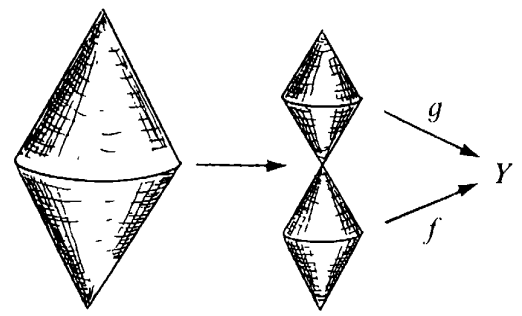
\includegraphics[width=0.6\textwidth]{Figures/TKISO0932.png}
      \caption{The product of two map classes
      $SX \to Y$.}
      \label{fig:TKISO0932-png}
  \end{figure}


  For a map $f \colon \left( SX, \left\{ A \right\}  \right) 
  \to \left( Y, \left\{ y_0 \right\}  \right) $, we denote its
  homotopy class in
  $\left[ SX; Y \right]_{*}$ by
  $\left[ f \right] $, and we define
  \[
  \left[ f \right] \left[ g \right] =
  \left[ f*g\right] 
  \] 
  Under this operation, the set
  $\left[ SX;Y \right]_*$ becomes a group.

  \begin{proposition}[]
      The reduced suspension gives
      $S S^{n-1}\cong S^{n}$.
  \end{proposition}

  Thus, we can define $S^{n}$ as the $n$-fold reduced
  suspension of $S^{0}$. As a special case,
  the set $\left[ S^{n};Y \right]_*$ then becomes
  a group for $n>0$. 

  \begin{definition}[$n$ th homotopy group]
      We define
      \[
      \pi_n \left( Y, y_0 \right) =
      \left[ S^{n}; Y \right]_*
      \] 
      with this operation.
  \end{definition}

  \subsection{Homotopy Groups using H-Spaces/Groups/Cogroups}

  From now on, unless otherwise indicated, we regard
  the $n$-sphere $S^{n}$ as having the cogroup
  structure as the reduced suspension
  $S^{n} = S S^{n-1} = S^{n-1} \wedge S^{1}$ - i.e.,
  the map $\gamma$ in the definition of an H-cogroup will
  be $\gamma \colon S^{n} \to S^{n} \vee S^{n}$ 
  given by
  \[
  \gamma(t,x) = 
  \begin{cases}
      \left( 2t,x \right)_{1},& t\le \frac{1}{2}\\
      \left( 2t-1, x \right)_2,& t\ge \frac{1}{2}.
  \end{cases}
  \] 
  The
  $0$-sphere $S^{0}$ is $\left\{ 0,1 \right\} $ 
  with base point $\left\{ 0 \right\} $.\\

  For a based space $X$ with base point $x_0$, we define
  the nth homotopy group
  \[
  \pi_n (X,x_0) = 
  \left[ S^{n},* ; X, x_0 \right] .
  \] 
  This is a group with the product defined by
  Theorem \ref{Thm:H-group-cogroup}.(2).

  \begin{theorem}[]\label{Theorem:Htpy-Groups-Abelian}
      If $X$ is an H-space then the multiplication
      in $\pi_n (X,x_0)$ is induced by
      the H-space multiplication and is abelian for
      $n\ge 1$.
  \end{theorem}

  \begin{proof}
      This follows directly from Theorem \ref{Thm:H-group-cogroup}.
  \end{proof}

  \begin{lemma}[]\label{Lemma:Suspension-Loop-Space}
      In the pointed category,
      $\left[ SX ; Y \right] \cong
      \left[ X ; \Omega Y \right]$ as groups.
  \end{lemma}
  
  \begin{proof}
      Recall the characteristic correspondence for
      the compact-open topology (Theorem \ref{Thm:Compact-Open-Top}):
      \[
      f\colon X \times S^{1} \to Y 
      \leftrightarrow f' \colon X \to Y^{S^{1}}
      \] 
      given by
      $f'(x) (t) = f(x,t)$.
      Recall that $SX = X \wedge S^{1}$, so
      a map
      $g \colon X \wedge S^{1} \to Y$ induces a map
      $f \colon X \times S^{1} \to Y$ by
      the composition 
      $X \times S^{1} \to X \wedge S^{1} \stackrel{g}{\to} Y$.
      Then $f$ is continuous if and only if
      the map $f' \colon X \to Y^{S^{1}}$ is continuous, where
      $f'(x)(*) = f(x,*) = *$, so
      $f'(*) = * \in Y^{S^{1}}$, the basepoint
      of $\Omega Y$.
      So the correspondence induces a bijective
      correspondence between pointed maps
      $SX \to Y$ and pointed maps $X \to \Omega Y$, and
      pointed homotopies correspond as well.\\
      It remains to show that the correspondence
      is a group homomorphism.
      Recall that $SX$ is an H-cogroup and
      $\Omega X$ is an H-group, so using
      Theorem \ref{Thm:H-group-cogroup}, we
      get that 
      for $f,g \colon SX \to Y$, the product in
      $\left[ SX;Y \right] $ is induced by
      \[
          \left( f*g \right) (x,t) = 
          \begin{cases}
              f(x,2t),& t\le \frac{1}{2}\\
              g\left( x,2t-1 \right),& t\ge \frac{1}{2},
          \end{cases}
      \] 
      which is equal to
      $\left( f*g \right)'(x)(t)$, 
      while the multiplication in
      $\left[ X ; \Omega Y \right] $ is given by
      $\left( f' \cdot g' \right) (x) = 
      f'(x) * g'(x)$ where $*$ is loop concatenation. 
      At time $t$, this is
      $f'(x) (2t)$ for $t\le \frac{1}{2}$ and
      $g'(x) (2t-1)$ for $t\ge \frac{1}{2}$. Thus
      $\left( f*g \right) ' = f' \cdot  g'$.
  \end{proof}


  All of the above immediately carries over to pointed
  pairs $(X,A)$ with a base point in $A$, so
  $\left[ SX, SA ; Y,B \right] $ is a group that
  is canonically isomorphic to
  $\left[ X,A; \Omega Y, \Omega B \right] $.

  Note in particular that
  $D^{n} \cong S D^{n-1}$ for all $n\ge 2$, so
  $D^{n} = D^{1} \wedge S^{n-1} \supset 
  S^{0} \wedge S^{n-1} = S^{n-1}$, so
  $\left( D^{n}, S^{n-1} \right) 
  = S^{n-1} \left( D^{1}, S^{0} \right) $, the
  $(n-1)$-fold reduced suspension. Hence
  we can define the relative homotopy group by
  \[
  \pi_n \left( Y,B,* \right) =
  \left[ D^{n}, S^{n-1}; Y ,B \right] 
  = \left[ S^{n-1}\left( D^{1}, S^{0} \right) ;
  Y,B\right] .
  \] 
  Note that this is defined on pointed spaces and pointed maps,
  so this set is really
  $\left[ D^{n},S^{n-1},s_0; Y,B, * \right] $.
  This becomes a group for $n\ge 2$. 

  Next note that we have a quotienting map
  \[
      I^{n} = \underbrace{D^{1}}_{=I} \times I \times \ldots \times I
      \to D^{1} \wedge S^{1} \wedge \ldots
      \wedge S^{1} =
      D^{n}.
  \] 
  Under this map, 
  $\partial I^{n}$ corresponds to
  $S^{n-1}$ and
  the base point corresponds to
  $J^{n-1} = \left( I \times \partial I^{n-1} \right) 
  \cup  \left( \left\{ 0 \right\} \times I^{n-1} \right) $.
  Thus under this quotienting map, we obtain a
  bijection
  \[
  \pi_n(Y,B,*) =
  \left[ D^{n}, S^{n-1},s_0; Y,B, * \right] 
  \cong \left[ I^{n}, \partial I^{n}, J^{n-1};
  Y,B,*\right].
  \] 

  \begin{corollary}
      $\pi_n(Y,*)$ is abelian for
      $n\ge 2$ and $\pi_n (Y,B,*)$ is abelian for
      $n\ge 3$. Moreover, the group structure is
      independent of the suspension coordinate used
      to define it.
  \end{corollary}

  \begin{proof}
      Recall from Lemma \ref{Lemma:Suspension-Loop-Space}, that
      $\left[ S^{n};Y \right] 
      = \left[ S^{1} \wedge \ldots \wedge S^{1};Y \right] 
      \cong \left[ S^{n-1} ; \Omega Y \right] $ as
      groups. Now
      the loop structure corresponds to the suspension in
      the last coordinate by definition, and
      by Theorem \ref{Thm:H-group-cogroup}, this
      is the same as the group 
      $\left[ S^{n};Y \right] $ with the suspension
      operation on any of the coordinates, since
      the choice of coordinate is arbitrary, this
      shows that
      the group structure on $\pi_n(Y,*) =
      \left[ S S^{n-1};Y \right]
      = \left[ S^{1} \wedge \ldots \wedge
      S^{1}; Y \right] $ is independent
      of the suspension coordinate used to define it.\\
      The product in $\left[ S^{n-1}; \Omega Y \right] $ is
      furthermore abelian for $n-1 \ge 1$ by
      Theorem \ref{Theorem:Htpy-Groups-Abelian} (using that
      $\Omega Y$ is an H-space), and
      the relative case is similar.
  \end{proof}

  \begin{corollary}
      \[
      \pi_n\left( Y,* \right) \cong
      \pi_{n-1}\left( \Omega Y, * \right) 
      \cong \ldots \cong
      \pi_1\left( \Omega^{n-1}Y,* \right) 
      \cong \pi_0 \left( \Omega^{n}Y ,* \right) 
      \] 
      and similarly in the relative case.
  \end{corollary}

  \begin{theorem}[]\label{Thm:Bredon-4.5}
      Let $A$ be a closed subspace of $X$ containing the
      base point $*$. Suppose that $F \colon X \times I \to X$ 
      is a deformation of $X$ contracting $A$ to
      $*$ ; i.e.,
      \begin{align*}
          F(A \times I) 
          &\subset A\\
          F(x,0) 
          &= x\\
          F\left( A \times \left\{ 1 \right\}  \right) 
          &= *\\
          F\left( \left\{ * \right\} \times I \right) 
          &= *
      \end{align*}
      then the quotient map $X \to X /A$ is a homotopy equivalence.
      Similarly for pairs $\left( X,X' \right) $ with
      $A \subset X'$.
  \end{theorem}

  \begin{proof}
      Let
      $\psi \colon X / A \to X$ be defined by the
      commutative diagram
      \begin{equation*}
      \begin{tikzcd}
          X \ar[d, "\varphi "] 
          \ar[dr, "F_{X \times \left\{ 1 \right\} } "]& \\
          X / A \ar[r, "\psi"] & X
      \end{tikzcd}
      \end{equation*}
      We claim that. Let $\varphi \colon X \to X / A$ be
      the quotienting map. We claim that
      $\psi \varphi \simeq \id_{X}$ and
      $\varphi \psi \simeq \id_{X / A}$.
      Since $F\left( A \times I \right) \subset A$, 
      $F$ induces a homotopy
      $F' \colon X / A \times I \to X / A$, where
      $F_{X / A \times \left\{ 1 \right\} }
      = \varphi \psi $, so
      since $F_{X / A \times \left\{ 0 \right\} }
      = \id_{X / A}$, we get the result.
  \end{proof}


  \newpage




  \subsubsection{A different way of defining
  $\pi_n \left( Y, y_0 \right) $}
  Note that reduced suspension supplies a parameter in
  $\left[ 0,1 \right] $ and the space
  $S^{n}$ as constructed is the quotient space of
  $I^{n}$ obtained by collapsing the boundary of the cube to a
  point.
  Pointed maps $S^{n}\to Y$ are in bijective correspondence
  with maps $I^{n}\to Y$ taking $\partial I^{n}$ to
  the base point of $Y$. This is a more traditional way
  of defining $\pi_n(Y)$. This becomes the group
  of homotopy classes of maps
  $\left( I^{n},\partial I^{n} \right) \to 
  \left( Y, \left\{ y_0 \right\}  \right) $ with the
  operation being
  \[
  f*g \left( t_1, \ldots, t_n \right) =
  \begin{cases}
      f\left( 2t_1, t_2, \ldots, t_n \right) ,& t_1 \in 
      \left[ 0,\frac{1}{2} \right] \\
      g\left( 2t_1-1, t_2, \ldots, t_n \right) ,& t_1 \in 
      \left[ \frac{1}{2},1 \right] 
  \end{cases}.
  \] 

  \begin{proposition}[]
      For $n\ge 2$, $\pi_n\left( X, x_0 \right)$ is abelian.
  \end{proposition}

  \begin{proof}
      Consider the homotopy in Figure \ref{fig:JIDWOOL0290L-png}.
      We begin by shrinking the domains of $f$ and $g$ to smaller
      subcubes of $I^{n}$, where the region outside is
      mapped to the basepoint. This allows us to move the boxes
      around in a continuous manner. The rest is clear.
      \begin{figure}[htpb]
          \centering
          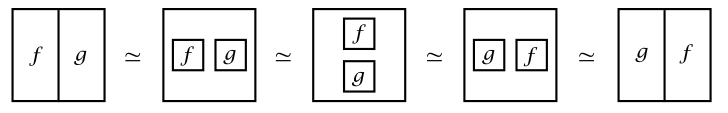
\includegraphics[width=0.8\textwidth]{Figures/JIDWOOL0290L.png}
          \caption{The homotopy in question}
          \label{fig:JIDWOOL0290L-png}
      \end{figure}
  \end{proof}

  Next, we want to show that following:
  \begin{proposition}[]\label{Prop:SwjiaKKDNW1102}
      If $X$ is path-connected, then
      $\pi_n\left( X, x_0 \right) \cong
      \pi_n (X, x_1)$ for any two $x_0,x_1 \in X$.
  \end{proposition}

  For this, we introduce an action of
  $\pi_1$ on $\pi_n$.

  \begin{definition}[The action of $\pi_1$ on $\pi_n$]
      Given a path
      $\gamma \colon I \to X$ from
      $x_0$ to $x_1$, we associate to a map
      $f \colon \left( I^{n}, \partial I^{n} \right) \to 
      \left( X, x_1 \right) $ the map
      $\gamma f \colon \left( I^{n}, \partial I^{n} \right) 
      \to \left( X,x_0 \right) $ by shrinking the domain
      of $f$ to a smaller concentric cube in $I^{n}$, then
      inserting the path $\gamma$ on each radial segment
      in the shell between this smaller cube and $\partial
      I^{n}$.
      See Figure \ref{fig:JDWIXHHX011SJ-png}

      \begin{figure}[htpb]
          \centering
          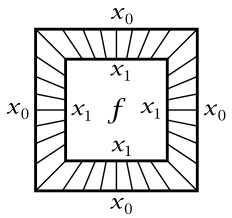
\includegraphics[width=0.25\textwidth]{Figures/JDWIXHHX011SJ.png}
          \caption{Depiction of $\gamma f$.}
          \label{fig:JDWIXHHX011SJ-png}
      \end{figure}

  \begin{note}
      We have the following properties
      \begin{enumerate}
          \item $\gamma \left( f+ g \right) 
              \simeq \gamma f + \gamma g$.
          \item $\left( \gamma \eta \right) f \simeq
              \gamma \left( \eta f \right) $.
          \item $\id f \simeq f$, where
              $\id$ denotes the constant path.
      \end{enumerate}

      To see $(1)$, first deform $f$ and $g$ to be
      constant on the right and left halves of
      $I^{n}$, respectively, producing maps
      which we may call $f+0$ and $0+g$, then we 
      can excise a progressively wider symmetric middle slab
      of $\gamma (f+0) + \gamma(0+g)$ (which can be
      seen on the left in Figure \ref{fig:WIWIWSSK11-png})
      until it becomes $\gamma \left( f+g \right) $ (shown on the
      right).

      \begin{figure}[htpb]
          \centering
          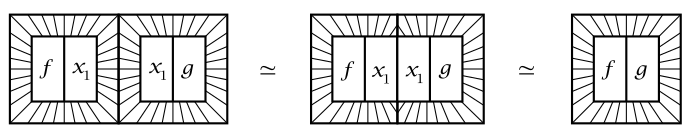
\includegraphics[width=0.8\textwidth]{Figures/WIWIWSSK11.png}
          \caption{}
          \label{fig:WIWIWSSK11-png}
      \end{figure}
  \end{note}

  Now if $\beta_{\gamma} \colon \pi_n(X,x_1) \to 
  \pi_n(X, x_0)$ is the change-of-basepoint transformation,
   $\beta_{\gamma}\left[ f \right] =
   \left[ \gamma f \right] $, then
   the above note shows that $\beta_\gamma$ is a group isomorphism.
   This proves Proposition \ref{Prop:SwjiaKKDNW1102}. 
   If we restrict attention to loops
   $\gamma$ at $x_0$, then since $\beta_{\gamma \eta}=
   \beta_{\gamma} \beta_{\eta}$, the map
   $\left[ \gamma \right] \mapsto \beta_{\gamma}$ 
   defines a homomorphism from
   $\pi_1\left( X, x_0 \right) $ to
   $\Aut \left( \pi_n \left( X,x_0 \right)  \right) $ 
   called the \textit{action of $\pi_1$ on $\pi_n$ }.
  \end{definition}

  \begin{note}
  For $n>1$, this action makes
  $\pi_n(X,x_0)$ into a module over the group ring
  $\mathbb{Z}\left[ \pi_1 \left( X,x_0 \right)  \right] $.
  \end{note}  

  \begin{definition}[Simple/abelian spaces]
      A space with trivial $\pi_1$ action on $\pi_n$ is called
      '$n$-simple', and 'simple' means
      ' $n$-simple for all $n$ '. We call
      a space \textit{abelian} if it has
      trivial action of $\pi_1$ on all homotopy groups
      $\pi_n$.
  \end{definition}

  \begin{proposition}[$\pi_n$ is a functor]
      A map $\varphi  \colon \left( X, x_0 \right) \to 
      \left( Y, y_0 \right) $ induces a map
      $\varphi_* \colon \pi_n \left( X, x_0 \right) \to 
      \pi_n \left( Y, y_0 \right) $ defined by
      $\varphi_* \left[ f \right] = \left[ \varphi  f \right] $.
      It is immediate from the definitions that
      $\varphi_*$ is well-defined and a homomorphism
      for $n\ge 1$. The functorial properties are also clear.
  \end{proposition}

  \begin{corollary}
      Homotopy equivalent spaces have isomorphic
      homotopy groups.
  \end{corollary}

  \begin{proposition}[]
      A covering space projection
      $p \colon \left( \tilde{X}, \tilde{x}_0 \right) \to 
      \left( X, x_0 \right) $ induces isomorphisms
      $p_* \colon \pi_n \left( \tilde{X}, \tilde{x}_0 \right) 
      \to \pi_n \left( X, x_0 \right) $ for all
      $n \ge 2$.
  \end{proposition}

  \begin{proof}
      Since 
      $S^{n}$ is path-connected and locally path-connected,
      and simply connected for $n\ge 2$, we find that
      any map
      $\left( S^{n},s_0 \right) 
      \to \left( X, x_0 \right) $ lifts to a 
      map $\left( S^{n},s_0 \right) \to 
      \left( \tilde{X},\tilde{x}_0 \right) $ when
      $n\ge 2$. This gives surjectivity of
      $p_*$.
      For injectivity, suppose
      $p_* \left[ f \right] = \left[ 0 \right] $ where
      $f \colon \left( S^{n}, s_0 \right) \to 
      \left( \tilde{X},\tilde{x}_0 \right) $.
      Let $c_{\tilde{x}_0}$ be the constant map at
      $\tilde{x}_0$. Then
      $p_* \left[ \tilde{x}_0 \right] =
      \left[ 0 \right] $, so by uniqueness of the
      lifting theorem, 
      $\left[ f \right] = \left[ c_{\tilde{x}_0} \right] =
      \left[ 0 \right] $.
  \end{proof}

  \begin{definition}[Aspherical]
      Spaces with $\pi_n = 0$ for all
      $n\ge 2$ are called \textit{aspherical}.
  \end{definition}

  \begin{corollary}
      $S^{1}, T^{n}$ and $K$ are aspherical since
      they have contractible covering spaces.
  \end{corollary}


  \begin{proposition}[]
      \[
      \pi_n \left( \prod_{\alpha} X_{\alpha} \right) 
      \cong \prod_{\alpha} \pi_n \left( X_{\alpha} \right) 
      \] 
  \end{proposition}

  Next we define relative homotopy groups.

  \begin{definition}[Relative homotopy groups]
      Regard $I^{n-1}$ as a face of $I^{n}$ with the last
      coordinate $s_n = 0$ and let
      $J^{n-1}$ be the closure of
      $\partial I^{n}- I^{n-1}$. Then
      we define 
      \[
      \pi_n \left( X, A, x_0 \right) 
      := \left[ I^{n},\partial I^{n}, J^{n-1};
      X , A , x_0\right] 
      \] 
      We shall leave $\pi_0 \left( X, A, x_0 \right) $ undefined
      for now.
  \end{definition}

  We can define a sum operation on $\pi_n \left( X, A, x_0 \right) $ 
  in the same way as for $\pi_n \left( X, x_0 \right) $, except
  now the coordinate $s_n$ now must remain free, so
  we must use one of the other coordinates. Thus
  we must have at least one other coordinate to define
  the same operation. So $\pi_n \left( X, A, x_0 \right) $ is
  a group for $n\ge 2$, and it is abelian for
  $n\ge 3$. For $n=1$, we have
  $I^{1} = \left[ 0,1 \right] , I^{0} = \left\{ 0 \right\} $ 
  and $J^{0} = \left\{ 1 \right\} $, so
  $\pi_1 \left( X, A, x_0 \right) 
  = \left[ I, \left\{ 0 \right\} , \left\{ 1 \right\} ;
  X, A, x_0 \right] $ is the set of homotopy classes of paths in
  $X$ from a varying point in $A$ to the fixed basepoint
  $x_0 \in A$. In general, this is not a group in any
  natural way. \\
  \linebreak
  Now, we saw before that
  $\pi_n \left( X, x_0 \right) $ can be regarded as
  homotopy classes of maps $\left( S^{n}, x_0 \right) \to 
  \left( X, x_0 \right) $. Similarly, collapsing
  $J^{n-1}$ to a point, converts
  $\left( I^{n} , \partial I^{n}, J^{n-1} \right) $ 
  to $\left( D^{n}, S^{n-1}, s_0 \right) $.
  In this case, addition is done by
  the map $c \colon D^{n} \to D^{n} \vee D^{n}$ collapsing
  $D^{n-1} \subset D^{n}$ to a point.\\
  \linebreak
  \begin{theorem}[Compression criterion]\label{Thm:Compression}
      A map $f \colon \left( D^{n}, S^{n-1}, s_0 \right) 
      \to \left( X, A, x_0 \right) $ represents zero
      in $\pi_n \left( X, A, x_0 \right) $ if and only if
      it is homotopic $\rel S^{n-1}$ to a map with image
      contained in $A$.
  \end{theorem}
  
  \begin{proof}
      Suppose we have a homotopy
      $\rel S^{n-1}$ from $f$ to a map
      $g$, so
      $\left[ f \right] = \left[ g \right] $ in
      $\pi_n \left( X, A, x_0 \right) $. 
      Viewing $g$ as a map
      $\left( D^{n}, S^{n-1}, s_0 \right) 
      \to \left( X, A, x_0 \right) $ whose
      image is contained in $A$, we
      can construct the homotopy
      $H \colon D^{n} \times I \to X$ by
      $H(x,t) = g\left( (1-t) x + s_0 t \right) $ 
      which is a homotopy from $g$ to the
      constant map at $x_0$, hence
      $\left[ g \right]  = 0$ in $\pi_n (X, A, x_0)$.\\
      Conversely, if $\left[ f \right] = 0$ via
      a homotopy $F \colon D^{n} \times I \to X$ such that
      $F(x,0) = f(x)$ and
      $F(x,1) = x_0$ for all $x \in D^{n}$ and
      $F(x,t) \in A$ for all
      $x$ with $\left| x \right| = 1$ as well
      as $F(s_0,t) = x_0$ for all $t$. We can
      construct a homotopy
      using $F$ by restricting $F$ to a family of
      $n$-disks in $D^{n} \times I$ starting with
      $D^{n}\times \left\{ 0 \right\} $ and ending
      with the disk $D^{n} \times \left\{ 1 \right\} 
      \cup S^{n-1} \times I$, and where all the disks
      throughout the family have the same boundary.
      See Figure \ref{fig:DJIMMXKXO0O-jpeg} for a depiction
      of this homotopy.

      \begin{figure}[htpb]
          \centering
          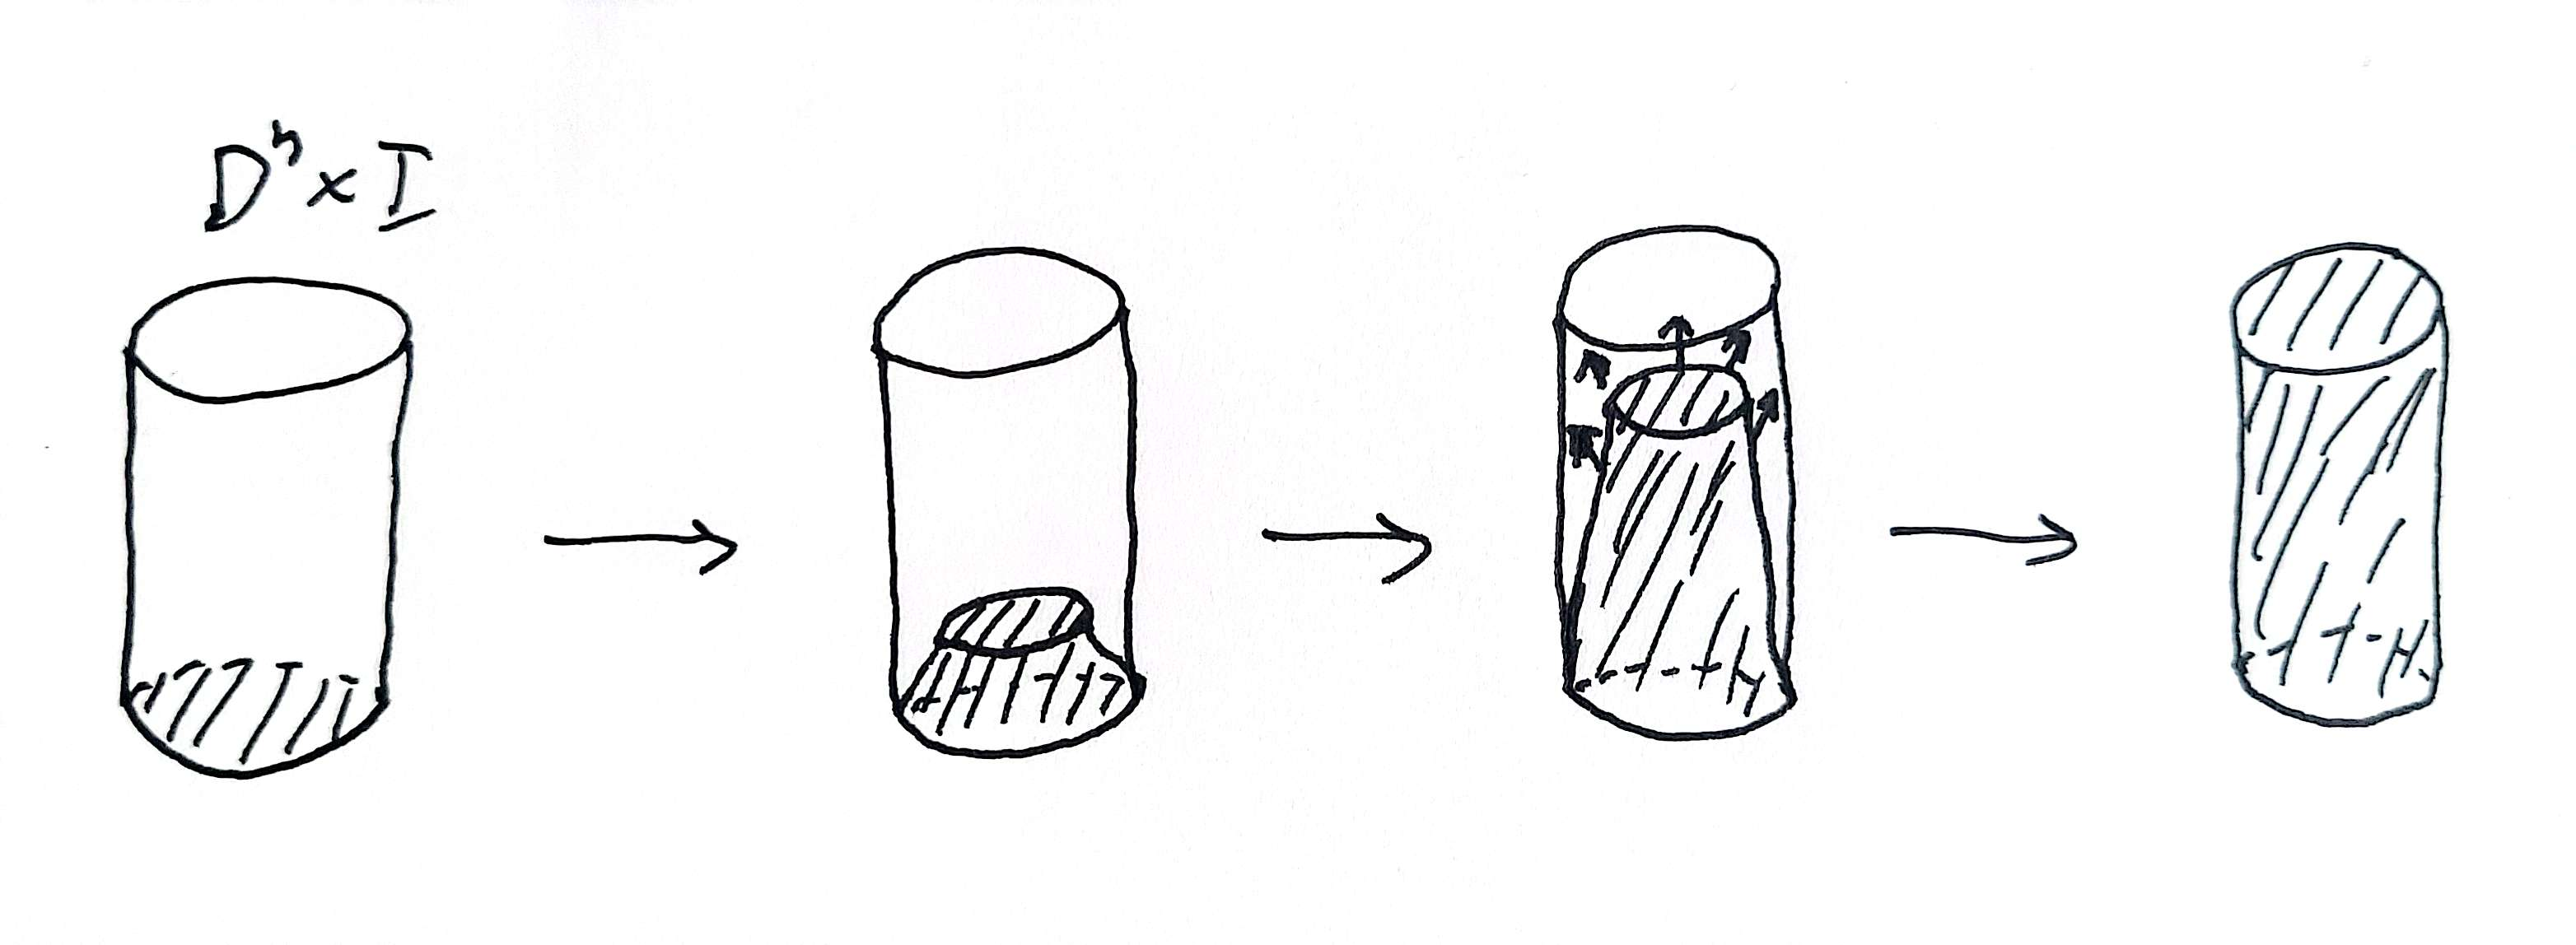
\includegraphics[width=0.8\textwidth]{Figures/DJIMMXKXO0O.jpeg}
          \caption{}
          \label{fig:DJIMMXKXO0O-jpeg}
      \end{figure}
      This completes the proof.
  \end{proof}

  Next, some things that carry over:
  a map $\varphi \colon \left( X, A, x_0 \right) 
  \to \left( Y, B, y_0 \right) $ induces maps
  $\varphi_* \colon \pi_n \left( X, A, x_0 \right) 
  \to \pi_n \left( Y, B, y_0 \right) $ which are
  homomorphisms when $n\ge 2$ and have properties analogous
  to those in the absolute case: 
  $\left( \varphi \psi  \right)_* = 
  \varphi_* \psi_*, (\id_{(X,A,x_0)})_{*} = \id_{\pi_n (X, A, x_0)}$,
  and if  $\varphi \simeq \psi $ through maps
  $\left( X,A,x_0 \right) \to \left( Y,B,y_0 \right) $,
  then $\varphi_* = \psi_*$. 

  \subsubsection{LES of relative homotopy groups}
  Probably the most useful feature of relative homotopy
  groups $\pi_n (X,A,x_0)$ is that they 
  fit into a long exact sequence
  \[
  \ldots \to \pi_n (A,x_0)
  \stackrel{i_*}{\to} \pi_n(X,x_0)
  \stackrel{j_*}{\to} \pi_n (X,A,x_0)
  \stackrel{\partial}{\to} \pi_{n-1}(A,x_0) \to 
  \ldots \to \pi_0 (X,x_0).
  \] 
  Here $i$ and $j$ are the inclusions
  $\left( A, x_0 \right) \hookrightarrow
  (X,x_0)$ and
  $\left( X, x_0, x_0 \right) \hookrightarrow
  \left( X,A,x_0 \right) $. The map
  $\partial$ comes from restricting maps
  $\left( I^{n},\partial I^{n}, J^{n-1} \right) \to 
  \left( X,A,x_0 \right) $ to
  $I^{n-1}$ (the face of $I^{n}$ with the last
  coordinate $s_n = 0$ ),
  or equivalently, by restricting maps
  $\left( D^{n},S^{n-1},s_0 \right) \to 
  \left( X,A,x_0 \right) $ to $S^{n-1}$. The map $\partial$,
  called the \textit{boundary map}, is a homomorphism
  when $n>1$. In fact, we can show the following theorem

  \begin{theorem}[LES of relative homotopy groups]
      Given 
      $x_0 \in B \subset A \subset X$,
      the sequence of relative homotopy groups
  \[
      \ldots \to 
      \pi_n \left( A,B, x_0 \right) 
      \stackrel{i_*}{\to} 
      \pi_n \left( X, B, x_0 \right) 
      \stackrel{j_*}{\to} 
      \pi_n (X, A, x_0)
      \stackrel{\partial}{\to} 
      \pi_{n-1} \left( A,B, x_0 \right) 
      \to \ldots \to 
      \pi_1 (X,A,x_0)
  \] 
  is exact and natural.
  In the case when $B = \left\{ x_0 \right\} $, we have that
  the LES
  \[
  \ldots \to \pi_n (A,x_0)
  \stackrel{i_*}{\to} \pi_n(X,x_0)
  \stackrel{j_*}{\to} \pi_n (X,A,x_0)
  \stackrel{\partial}{\to} \pi_{n-1}(A,x_0) \to 
  \ldots \to \pi_0 (X,x_0).
  \] 
  is exact and natural.
  \end{theorem}

  \begin{proof}
      \textit{Exactness at $\pi_n
      \left( X,B,x_0 \right) $ :} the composition
      $j_* i_*$ is zero because any
      map $\left( I^{n}, \partial I^{n},
      J^{n-1}\right) \to \left( A,B,x_0 \right) $ 
      is zero in $\pi_n \left( X, A, x_0 \right) $ by the
      compression criterion (Theorem \ref{Thm:Compression}).
      To see that $\ker j_* \subset 
      \im i_*$, let
      $f \colon \left( I^{n}, \partial I^{n},
      J^{n-1}\right) \to \left( X, B, x_0 \right) $ 
      represent zero in $\pi_n \left( X, A, x_0 \right) $.
      Using the compression criterion again, we
      then get that $f$ is homotopic $\rel \partial I^{n}$ 
      to a map with image in $A$, hence the class
      $\left[ f \right] \in \pi_n \left( X, B, x_0 \right) $ 
      is indeed in the image of $i_*$. We conclude that
      $\ker j_* = \im i_*$, obtaining exactness
      at $\pi_n \left( X,B, x_0 \right) $.\\
      \textit{Exactness at $\pi_n (X,A,x_0)$:} 
      for a map  $\left[ f \right] 
      \in \im j_*$, we have that
      $j_*$ maps $\partial I^{n}$ into $B$, hence
      in particular $I^{n-1} \subset \partial I^{n}$ into
      $B$, so $\partial j_* \left[ f \right] $ 
      represents a homotopy class
      in $\pi_{n-1}\left( A,B,x_0 \right) $ with
      image in $B$, but then by the compression criterion,
      $\partial j_* \left[ f \right] = 0$ in
      $\pi_{n-1} \left( A,B,x_0 \right) $, so
      $\im j_* \subset \ker \partial $.
      Conversely, suppose
      $\partial \left[ f \right] = 0$. By the compression
      criterion, representatives of $\partial \left[ f \right] $
      are homotopic $\rel \partial I^{n-1}$ to a map
      with image in $B$. In particular,
      $f|_{I^{n-1}}$ is homotopic to a map with
      image in $B$ via a homotopy $F \colon
      I^{n-1} \times I \to A \rel \partial I^{n-1}$.
      We can tack $F$ onto $f$ to get a new map
      $\left( I^{n}, \partial I^{n},
      J^{n-1}\right) \to 
      \left( X, B, x_0 \right) $ which, as
      a map
      $\left( I^{n}, \partial I^{n}, J^{n-1} \right) \to 
      \left( X, A, x_0 \right) $ is homotopic to
      $f$ by the homotopy that tacks on increasingly longer
      initial segments of $F$. See Figure
      \ref{fig:IDIWKAKX-png}. Hence
      $\left[ f \right] \in \im j_*$.

      \begin{figure}[htpb]
          \centering
          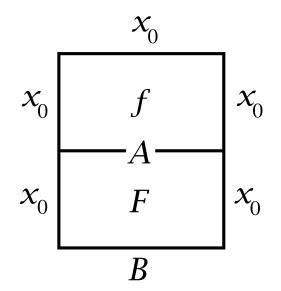
\includegraphics[width=0.2\textwidth]{Figures/IDIWKAKX.png}
          \caption{}
          \label{fig:IDIWKAKX-png}
      \end{figure}

      \textit{Exactness at $\pi_n (A,B,x_0)$ :} 
      First, $i_* \partial$ is zero since
      the restriction of a map
      $f \colon \left( I^{n+1}, \partial I^{n+1},
      J^{n}\right) \to \left( X,A,x_0 \right) $ 
      to $I^{n}$ is homotopic $\rel \partial I^{n}$ to a 
      constant map via $f$ itself (a similar picture
      to Figure \ref{fig:DJIMMXKXO0O-jpeg} works).\\
      Conversely, if $B$ is a point, then
      a nullhomotopy $f_t \colon
      \left( I^{n}, \partial I^{n} \right) 
      \to \left( X, x_0 \right) $ of
      $f_0 \colon \left( I^{n},\partial I^{n} \right) 
      \to \left( A,x_0 \right) $ gives a map
      $F \colon \left( I^{n+1},\partial I^{n+1},J^{n} \right) 
      \to \left( X,A,x_0 \right) $ with
      $\partial \left( \left[ F \right]  \right) 
      = \left[ f_0 \right] $. So in this case, the proof is
      finished.
      For a general $B$, let
      $F$ be a nullhomotopy of
      $f \colon \left( I^{n},\partial I^{n},J^{n-1} \right) 
      \to \left( A,B,x_0 \right) $ through maps
      $\left( I^{n}, \partial I^{n}, J^{n-1} \right) 
      \to \left( X,B,x_0 \right) $ and
      let $g$ be the restriction of
      $F$ to $I^{n-1}$ in $I^{n-1} \times I = I^{n}$ (see
      the first of the pictures in
      Figure \ref{fig:USIIOOQ-png}).
      Next reparametrize the $n$ th and
      $(n+1)$ st coordinates as in the
      second picture. Then 
       we find that $f$ with $g$ tacked on
       is in the image of $\partial$. But
       as before, tacking $g$ onto $f$ gives the
       same element of $\pi_n (A,B,x_0)$

      \begin{figure}[htpb]
          \centering
          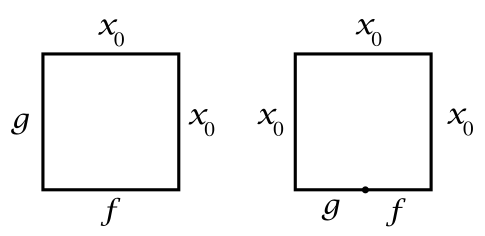
\includegraphics[width=0.4\textwidth]{Figures/USIIOOQ.png}
          \caption{}
          \label{fig:USIIOOQ-png}
      \end{figure}
  \end{proof}

  
\begin{corollary}
    Consider the inclusion
    $\iota \colon X = X \times \left\{ 0 \right\} 
    \hookrightarrow CX$.
    Then
    $\pi_n \left( CX, X, x_0 \right) 
    \cong \pi_{n-1}\left( X, x_0 \right) $ for all
    $n\ge 1$. Taking
    $n=2$, we can thus realize an group $G$, abelian
    or not, as a relative $\pi_2$ by
    choosing $X$ to have $\pi_1 (X) \cong G$.
\end{corollary}

There are also change-of-basepoint isomorphisms
$\beta_{\gamma}$ for relative homotopy groups.
One takes a path  $\gamma$ in $A \subset X$ from
$x_0$ to $x_1$ which induces
$\beta_{\gamma} \colon \pi_n (X,A,x_1) \to 
\pi_n (X,A,x_0)$ by setting
$\beta_{\gamma} \left( \left[ f \right]  \right) 
= \left[ \gamma f \right] $, where
$\gamma f$ is depicted in 
Figure \ref{fig:DIWIOA-png}.

\begin{figure}[htpb]
    \centering
    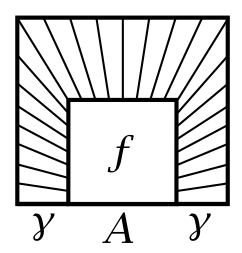
\includegraphics[width=0.2\textwidth]{Figures/DIWIOA.png}
    \caption{}
    \label{fig:DIWIOA-png}
\end{figure}

Restricting to loops at the
basepoint, the association $\gamma \mapsto 
\beta_{\gamma}$ defines an action
of $\pi_1 \left( A, x_0 \right) $ on
$\pi_n \left( X, A, x_0 \right) $ analogous to the
action of $\pi_1 \left( X, x_0 \right) $ on
$\pi_n (X,x_0)$.






%\subsection{Problem Set 1}

\subsubsection{Exercises}


\begin{exercise}[The action of the fundamental gorup, part
    2]
    Let $X$ be a path-connected, semi-locally simply-connected
    space with basepoint $x$ and $p \colon \tilde{X}\to X$ its
    universal cover. Show that for $n\ge 2$ and
     $\tilde{x} \in X$ with $p (\tilde{x}) = x$, the isomorphism
     $p_* = \pi_n (p) \colon \pi_n \left( \tilde{X}, \tilde{x} \right) 
     \cong \pi_n(X, x)$ allows us to identify the
     action of $\pi_1 \left( X, x \right) $ on $\pi_n (X, x)$ with
     the action of $\pi_1 \left( X, x \right) $ on
     $\pi_n \left( \tilde{X}, \tilde{x} \right) $ induced by
     the group of deck transformations, i.e., the natural action
     of $\pi_1 (X, x)$ on $\tilde{X}$. In particular, make the
     statement precise.
\end{exercise}

\begin{proof}
    We want to show that for $\left[ \gamma \right] 
    \in \pi_1(X, x)$ and
    $\left[ f \right] \in \pi_n \left( X, x \right) $,
    if $\tilde{g}$ is the lift for $\gamma$ starting at
    $\tilde{x}_0$, and
    $\tilde{f} \colon \left( S^{n}, s_0 \right) 
    \to \left( \tilde{X}, \tilde{x}_0 \right) $ is the
    lift of $f$, then
    $p_* \left( \tilde{\gamma} \tilde{f} \right) 
    = \gamma f$. But this follows directly from how
    $\tilde{\gamma} \tilde{f}$ and 
    $\gamma f$ we constructed. Namely, applying
    $p$ to the square used in the definition, we see that we
    obtain $\gamma f$ from $\tilde{\gamma} \tilde{f}$ since
    $p \circ \tilde{\gamma} = \gamma$ and
    $p \circ \tilde{f} = f$.

\end{proof}


\begin{exercise}[]
    Let $X$ and $Y$ be pointed spaces and $n \ge 2$. Show that the
    inclusion $X \vee Y \hookrightarrow X \times Y$ induces
    a surjection $\pi_n \left( X \vee Y \right) 
    \to \pi_n \left( X \times Y \right) $ for all $n$. Furthermore,
    this exhibits $\pi_n \left( X \times Y \right) $ as
    a retract of $\pi_n \left( X \vee Y \right) $ for all $n$.
    (Is this also true for $n=1$?)
\end{exercise}

\begin{proof}
    a
\end{proof}






\subsubsection{Problems}

\begin{problem}[]\label{pset1-degree}
        Fix an isomorphism $H_n\left( S^{n} \right) \cong \mathbb{Z}$.
        We define the degree $\deg f$ of a map
        $f \colon S^{n} \to S^{n}$ to be the integer such that
        $f_* \colon H_n(S^{n}) \to H_n(S^{n})$ sends $1$ to
        $\deg f \in \mathbb{Z}$.
        \begin{enumerate}
            \item Show that taking the degree of a map
                $S^{n} \to S^{n}$ induces a well-defined
                map
                \[
                \deg \colon \pi_n(S^{n}) \to \mathbb{Z}
                \] 
            \item Show that $\deg $ is a group homomorphism.
            \item Show that the map $\deg$ is surjective.
            \item Suppose that $n\ge 2$. Show that
                $\pi_n\left( S^{n} \right) \cong
                \mathbb{Z} \times A$ for some abelian group $A$.
        \end{enumerate}
    \end{problem}

        \begin{proof}


        \begin{enumerate}
            \item Let
                $ \left[ f \right] 
                \in \pi_n \left( S^{n} \right) $ and
                suppose $f, f'$ are two representatives of
                this class. Then
                $f$ and $f'$ are homotopic by definition,
                so $f_* = \left( f' \right)_* \colon
                \mathbb{Z} = H_n\left( S^{n} \right) \to 
                H_n\left( S^{n} \right) = \mathbb{Z} $ are equal.
                In particular,
                $\deg f = f_*(1) = \left( f' \right)_* (1)
                = \deg f'$. So the map is well-defined.
            \item To show that degree is a group homomorphism,
                we must show that
                $\deg \left( f+g \right) = 
                \deg f + \deg g$.

                For this, we will show a couple of results.

                \begin{proposition}[]
                    Let $X = S_1^{n} \vee \ldots \vee
                    S_k^{n}$ for $n > 0$. Then
                    the homomorphism 
                    $H_n\left( S_1^{n} \right) \oplus \ldots
                    \oplus H_n\left( S_k^{n} \right) 
                    \to H_n(X)$ induced by the inclusion maps
                    is an isomorphism whose inverse
                    is induced by the projections
                    $X \to S_i^{n}$.
                \end{proposition}
                
                To prove this proposition, we must show the following
                lemma.

                \begin{lemma}[]
                    Let $X$ be a Hausdorff space and let
                    $x_0 \in X$ be a point having a closed
                    neighborhood $N$ in $X$ of which
                    $\left\{ x_0 \right\} $ is a strong deformation
                    retract. Let $Y$ be a Hausdorff space and
                    let $y_0 \in Y$. Define
                    $X \vee Y = X \times \left\{ y_0 \right\} 
                    \cup \left\{ x_0 \right\} \times Y$.
                    Then the inclusion maps induce
                    isomorphisms 
                    $\tilde{H}_i(X) \oplus \tilde{H}_i(Y)
                    \cong \tilde{H}_i\left( X \vee Y \right) $
                    whose inverse is induced by the projections
                    of $X \vee Y$ to $X$ and $Y$.
                \end{lemma}
                
                \begin{proof}[Proof of lemma]
                    Consider $A = X$ and
                    $U = X - N$ which is open, and
                    $\overline{U} \subset A$. Then by
                    excision,
                    $H_* \left( X \vee Y, X \right) 
                    \cong H_*\left( N \cup Y, N \right) 
                    \cong \tilde{H}_*\left( Y \right) $

                    Consider the LES of the triple
                    $\left( X \vee Y,
                    \left\{ x_0 \right\} \times Y,
                \left\{ x_0 \right\} \times 
            \left\{ y_0 \right\} \right) $. We obtain
            \[
            \ldots \to 
            H_p\left( \left\{ x_0 \right\} \times Y,
            \left( x_0,y_0 \right) \right)
            \stackrel{i_*}{\to}
            H_p\left( X \vee Y, \left( x_0,y_0 \right)  \right) 
            \stackrel{j_*}{\to} H_p\left( X \vee Y,
            \left\{ x_0 \right\} \times Y \right) \to \ldots
            \] 
            Since $\pi_Y \circ i = \id_{
            \left\{ x_0 \right\} \times Y} $, 
            $i_*$ is injective.

            Furthermore, we have
            \[
            H_p\left( X \vee Y, 
            \left( x_0, y_0 \right) \right) 
            \stackrel{\left( \pi_X \right)_* }{\to } 
            H_p \left( \left\{ x_0 \right\} \times Y,
            \left( x_0, y_0 \right) \right) 
            \cong H_p\left( X \vee Y , 
            \left\{ x_0 \right\} \times Y \right) 
            \] 
            so $j_* = \left( \pi_X \right)_*$ under these
            identifications, so, in particular, 
            $j_*$ is surjective. Therefore, our exact sequence
            is a SES:
            \[
            0 \to  H_p\left( Y, pt \right)
            \stackrel{i_*}{\to }
            H_p \left( X \vee Y, pt \right) 
            \stackrel{j_*}{\to }
            \underbrace{H_p \left( X \vee Y, Y \right)}_{
            \cong H_p\left( X, pt \right) } \to 0
            \] 
            It remains to show that this SES is split, but
            since
            $\pi_X \circ \iota_{X} = 
            \id_{\left\{ x_0 \right\} \times X}$,
            we have that $\iota_{X*}$ provides a section.

        \end{proof}

        \begin{proof}[Proof of proposition]
            This follows by induction on the lemma.
        \end{proof}

        Next, suppose that $E_1, \ldots, E_k$ are
        disjoint open subsets of $S^{n}$, each homeomorphic to
        $\mathbb{R}^{n}$ for $n>0$.
        Let $f \colon S^{n} \to Y$ be a map which takes
        $S^{n} - \bigcup E_i $ to $y_0$. Then
        $f$ factors through the quotient space
        $S^{n} / \left( S^{n} - \bigcup E_i  \right) 
        \cong S_1^{n} \vee \ldots \vee S_k^{n}$ where
        $S_i^{n} = S^{n} / \left( S^{n} - E_i \right) $:
        \[
            f \colon S^{n} \stackrel{g}{\to }
            S_1^{n} \vee \ldots \vee S_k^{n}
            \stackrel{h}{\to } Y
        \] 
        Let $\iota_{j} \colon S_j^{n} 
        \hookrightarrow S_1^{n} \vee \ldots \vee
        S_k^{n}$ be the $j$ th inclusion and let
        $p_j \colon S_1^{n} \vee \ldots \vee
        S_k^{n} \to S_j^{n}$ be the $j$ th projection.
        Then by the proposition,
        $\sum_j \iota_{j*} p_{j*} = \id_* \colon
        H_n \left( S_1^{n} \vee \ldots \vee S_k^{n} \right) 
        \to H_n \left( S_1^{n} \vee \ldots \vee
        S_k^{n}\right) $. Let
        $g_j = p_j \circ g \colon S^{n} \to S_j^{n}$ and
        $h_j = h \circ \iota_j \colon
        S_j^{n} \to Y$ and let
        $f_j = h_j \circ g_j \colon  S^{n} \to Y$.
        That is, $f_j$ is the map which is $f$ on
        $E_j$ and maps the complement of $E_j$ to the basepoint
        $y_0$.

        \begin{theorem}[]\label{Thm:Degree-of-sum-of-maps}
            In the above situation, $f_*
            = \sum_{j=1}^{k} f_{j*} \colon
            H_n\left( S^{n} \right) \to H_n(Y)$.
        \end{theorem}

        \begin{proof}[Proof of theorem]
            We have
            $f_* = 
            h_* \circ g_* = 
            \sum_j h_* i_{j*} p_{j*} g_*
            = \sum_j h_{j*} g_{j*}
            = \sum_j f_{j*}$.
        \end{proof}

        Now we get back to showing that
        $\deg \left( f+g \right) = \deg f + \deg g$.

        Note that by way of defining
        $f+g$, this essentially maps $I^{n}$ by
        $f$ on the left half and $g$ on the right half with
        the boundary mapping to the base point $x_0$.
        In particular, this factors through the
        quotient $I^{n} \to I^{n} / \partial I^{n} 
        \cong S^{n}$, where now the two halves can be interpreted
        as, say, the upper and lower hemispheres. In particular,
        the equator is by assumption also mapped to
        $x_0$, so we can quotient further by
        $S^{n} \to S^{n} \vee S^{n}$ by "pinching" the equator
        to a point. This is essentially what the proposition
        above describes. In particular, $f+g$ can be covered
        by the two open hemispheres and maps the equator
        to $x_0$, so by the theorem,
        we have $\left( f+g \right)_*
        = f_* + g_*$, i.e.,
        $\deg (f+g) = \left( f+g \right)_*(1)
        = f_*(1) + g_*(1) = \deg f + \deg g$, as we wanted
        to show.

    \item 
        Next we show that $\deg$ is surjective. 
        First note that
        $\deg \id = \id_* (1) = 1$ by functoriality since
        $\id_* = \id_{H_n(S^{n})}$.
        By functoriality, we thus hit
        all of $\mathbb{Z}$. More precisely,
        $\deg \left( \ast_{n} \id \right) = n$ for
        $n \in \mathbb{N} $ as
        $\deg$ is a homomorphism.
        Also $\deg \left( \ast_{n} (-\id) \right) 
        = -n$ for $n \in \mathbb{N} $ and
        $\deg (c_{x_0}) = 0$, so
        $\deg$ is surjective.
    \item Let $n\ge 2$. We have a SES
        \[
        0 \to \ker \deg \to 
        \pi_n\left( S^{n} \right) \stackrel{\deg}{\to }
        \mathbb{Z} \to 0.
        \] 
        Since $\mathbb{Z}$ is projective, 
        this splits, so
        $\pi_n\left( S^{n} \right) 
        \cong \mathbb{Z} \oplus \ker \deg$.
        But $\ker \deg$ is a subgroup of
        $\pi_n\left( S^{n} \right) $ which is abelian, hence
        is itself abelian.







        \end{enumerate}

    \end{proof}


    \begin{problem}[]
        Fix $n\ge 1$. We say that a space $X$ is
        \textit{$n$-connected} if it is non-empty, path-connected,
        and $\pi_k (X, x) = 0$ for all $1 \le k \le n$ and
        $x \in X$.
        For $\left( X, x_0 \right) $ a pointed, path-connected space,
        show that the following are equivalent:
        \begin{enumerate}
            \item $X$ is $n$-connected.
            \item $\pi_k\left( X,x_0 \right) = 0$ for all
                $1 \le k \le n$.
            \item Every map
                $S^{k} \to X$ can be extended to a map
                $D^{k+1} \to X$ for all $k \le n$.
            \item Every map
                $S^{k} \to X$ is homotopic to a constant
                map for all
                $k \le n$.
        \end{enumerate}
    \end{problem}

    \begin{proof}
        $\left( 1 \implies 2 \right) $: this follows since
        $X$ being $n$-connected means that $\pi_k\left( X,x \right) 
        = 0$ for all $x \in X$ and all $1\le k\le n$,
        hence in particular for $x_0$.\\
        $(2 \implies 3)$ : Let
        $f \colon S^{k} \to X$ be a map. 
        Then $f$ represents some homotopy class
        $\left[ f \right] \in \pi_k\left( X,x_0 \right) $. But
        since $\pi_k(X,x_0) = 0$, $f$ is homotopic to
        the constant map at $x_0 \rel s_0$.
        Let $H \colon S^{k} \times I \to X$ be this homotopy.
        Define
        $\tilde{f} \colon D^{k+1} \to X$ by
        $\tilde{f}(x) = H \left( x, \|x\| \right) $.
        Then $\tilde{f}$ is continuous as a composite of
        continuous maps and
        $\tilde{f}|_{S^{k}}(-) = 
        H\left( - , 1 \right) =
        f(-)$, so $\tilde{f}$ indeed extends $f$.\\
        $(3 \implies 4)$ : Let $f \colon S^{k} \to X$ be
        a map. Extends $f$ to a map
        $\tilde{f} \colon D^{k+1} \to X$. Define now
        a homotopy
        $H \colon S^{k} \times I \to X$ by
        $H\left( x,t \right) =
        \tilde{f}\left( xt \right) $. This is continuous
        and $H\left( x,1 \right) =
        \tilde{f}(x) = f(x)$ while
        $H\left( x,0 \right) = 
        \tilde{f}(0) \in X$ is constant. Hence this gives
        a homotopy between $f$ and $c_{\tilde{f}(0)}$.\\
        \linebreak
        $(4 \implies 3)$ : 
        Let $f \colon S^{k} \to X$ be a given map.
        By assumption, there exists
        a homotopy
        $H \colon S^{k} \times I \to X$ such that
        $H\left( -,1 \right) = f(-)$ and
        $H(-,0) = c$ where $c$ is some constant map
        at a point in $X$.
        But then $H$ factors through the quotient
        \begin{equation*}
        \begin{tikzcd}
            S^{k} \times I \ar[d] \ar[dr, "H"] & \\
            D^{k+1} \ar[r, "\tilde{H}"'] & X
        \end{tikzcd}
        \end{equation*}
        where we identify
        $S^{k} \times \left\{ 0 \right\} $ to a point.
        But then $\tilde{H}|_{S^{k}} (-) = 
        H\left( -, 1 \right) =
        f(-)$, so $\tilde{H}$ extends $f$.\\
        \linebreak
        $(3 \implies 2)$ : 
        Let $\left[ f \right] \in \pi_k(X, x_0)$ and
        $f$ a representative. 
        We want to show that $f$ is homotopic to the
        constant map at $x_0$ relative $\partial I^{k}$.
        Extend $f$ to a map 
        $\tilde{f} \colon D^{k+1} \to X$, and let
        $H \colon S^{k} \times I \to X$ be given by
        $H\left( x,t \right) =
        \tilde{f}\left( ts_0 + (1-t) x \right) $. This gives
        a homotopy between $f$ and the constant map
        at  $x_0$.\\
        \linebreak
        $\left( 2 \implies 1 \right) $ : the only thing that
        requires showing is that
        given that $\pi_k(X, x_0) = 0$ for all $k$, we then
        have $\pi_k \left( X, x \right) = 0$ for all $k$ and
        all $x \in X$. But this is precisely what the given
        hint says we are allowed to assume since
        $X$ is path connected. So we are done.
    \end{proof}

    \begin{definition}[n-connected maps]
        A map $f \colon X \to Y$ is called \textit{n-connected}
        if it induces isomorphisms on all homotopy
        groups in degree $<n$ and an epimorphism
        in degree $n$.
    \end{definition}





    %\printbibliography


\begin{problem}[$n$-connected in the relative case]\label{n-connected-relative}
    The following four conditions are equivalent for
    $i>0$ :
    \begin{enumerate}
        \item Every map
            $\left( D^{i} , \partial D^{i} \right) \to 
            \left( X,A \right) $ is homotopic
            $\rel \partial D^{i}$ to a map $D^{i} \to A$.
        \item Every map $\left( D^{i},\partial D^{i} \right) 
            \to (X,A)$ is homotopic through such maps
            to a map $D^{i} \to A$.
        \item Every map $\left( D^{i}, \partial D^{i} \right) 
            \to \left( X,A \right) $ is homotopic through such
            maps to a constant map $D^{i} \to A$.
        \item $\pi_i \left( X, A, x_0 \right) = 0$ for all
            $x_0 \in A$.
    \end{enumerate}
    When $i = 0$, we did not define the relative $\pi_0$,
    and (1)-(3) are each equivalent to saying that
    each path-component of $X$ contains points
    in $A$ since $D^{0}$ is a point and
    $\partial D^{0}$ is empty. The pair
    $\left( X, A \right) $ is called \textit{$n$-connected}
    if (1)-(4) hold for $0<i\le n$ and
    (1)-(3) hold for  $i=0$.
\end{problem}


\subsection{Whitehead's Theorem}

\begin{theorem}[Whitehead's Theorem]\label{Thm:Whitehead}
    If a map $f \colon X \to Y$ between connected
    $CW$ complexes induces isomorphisms
    $f_* \colon \pi_n (X) \to \pi_n (Y)$ for all
    $n$, then $f$ is a homotopy equivalence.
    In case $f$ is the inclusion of a subcomplex
    $X \hookrightarrow Y$, the conclusion is stronger:
    $X$ is a deformation retract of $Y$.
\end{theorem}

The proof will require the following lemma:

\begin{lemma}[Compression Lemma]
    Let $\left( X,A \right) $ be a CW pair and let
    $\left( Y, B \right) $ be any pair with
    $B \neq \varnothing$. For each  $n$ such that
    $X - A$ has cells of dimension $n$, assume
    that  $\pi_n \left( Y, B, y_0 \right) = 0$ for
    all $y_0 \in B$. Then every map $f \colon
    \left( X,A \right) \to \left( Y,B \right) $ is homotopic
    $\rel A$ to a map $X \to B$.
    When $n = 0$, the condition that
    $\pi_n \left( Y,B,y_0 \right) =0$ for all
    $y_0 \in B$ is to be regarded as saying that
    $\left( Y,B \right) $ is $0$-connected.
\end{lemma}

\begin{proof}[Proof of lemma]
    Assume inductively that $f$ has already been
    homotoped to take the skeleton
    $X^{k-1}$ to $B$. Let
    $\Phi$ be the caracteristic (attaching) map of 
    cell $e^{k}$ of $X - A$. Then the composition
    $f \Phi \colon \left( D^{k} , \partial D^{k} \right) 
    \to \left( Y,B \right) $ is in some class
    in $\pi_k \left( Y, B, y_0 \right) = 0$, so
    it can be homotoped into $B \rel \partial D^{k}$ by
    the compression criterion when
    $k > 0$, or
    by $\left( Y,B \right) $ being $0$-connected for
    $k = 0$ (this is condition (3) in Problem \ref{n-connected-relative}).
    This homotopy of $f \Phi$ induces a homotopy
    $\rel X^{k-1}$ on the quotient space
    $X^{k-1} \cup e^{k}$ of $X^{k-1} \sqcup D^{k}$.
    Doing this for all $k$-cells of $X-A$ simultaneously, and
    taking the constant homotopy on $A$, we obtain a
    homotopy of $f|_{X^{k} \cup A}$ to a map into
    $B$. Since the inclusion of a
    subcomplex into a CW-complex is a cofibration,
    $f|_{X^{k} \cup  A}$ extends to all of $X$ (essentially
    the homotopy extension property).
    This completes the inductive step in the finite dimensional
    CW-complex case.
    In the general case, we perform the
    homotopy of the inductive step during the
    $t$-interval $\left[ 1- \frac{1}{2^{k}},
    1- \frac{1}{2^{k+1}}\right] $. Any finite skeleton
    $X^{k}$ is eventually stationary under these
    homotopies, hence we have a well-defined
    homotopy $f_t, t \in \left[ 0,1 \right] $ with
    $f_1 (X) \subset B$.
\end{proof}


\begin{proof}[Proof of Whitehead's Theorem, \ref{Thm:Whitehead}]
    Let's tackle the case when $f$ is the inclusion
    of a subcomplex first. Consider then
    the LES of the pair $\left( Y,X \right) $. Since
    $f$ by assumption induces isomorphisms
    on all homotopy groups,
    $f_* \colon \pi_* (X) \to \pi_* (Y)$, the
    relative homotopy groups
    $\pi_* (Y,X)$ are zero. Applying the lemma now
    to the identity map $\left( Y,X \right) \to 
    \left( Y,X \right) $, we obtain a homotopy
    of the identity  $\id \colon Y \to Y$ to
    a map $Y \to X$ which is relative to
    $X$. That is, we obtain a deformation retract of
    $Y$ onto $X$.\\
    \linebreak
    For the general case, recall that
    a map $f \colon X \to Y$, can be considered
    as the composition of the
    inclusion $X \hookrightarrow M_f$ and the
    retraction $M_f \to Y$. Since
    the retraction is a homotopy equivalence,
    it suffices to show that $M_f$ deformation retracts
    onto $X$ if $f$ induces isomorphisms on homotopy
    groups, or equivalently, if the relative groups
    $\pi_n \left( M_f, X \right) $ are all zero (since
    $M_f \simeq Y$ ).
    If $f$ is cellular - i.e., takes the $n$-skeleton of
    $X$ to the $n$-skeleton of $Y$ for all
    $n$ - then $\left( M_f, X \right) $ is a CW pair and
    we can apply the first paragraph of the proof.\\
    If $f$ is not cellular, we can either apply
    Theorem 4.8 in \cite{Hatcher} which says
    that $f$ is homotopic to a cellular map, or we can use
    the following argument.

    First, using that 
    $\pi_n \left( M_f, X \right) = 0$ for all $n$, 
    apply the Compression Lemma to
    the inclusion $ \left( X \cup  Y, X \right) 
    \hookrightarrow \left( M_f, X \right) $ to
    obtain a homotopy of the
    inclusion to a map into $X \rel X$.
    The inclusion $X \cup Y \hookrightarrow M_f$ can be
    seen to be a cofibration using 
    Theorem \ref{Thm:SJJDHW29WW}, so
    the pair $\left( M_f, X \cup Y \right) $ satisfies the
    homotopy extension property. So the
    homotopy in question extends to a homotopy
    from the identity of $M_f$ to a
    map $g \colon M_f \to M_f$ taking 
    $X \cup Y$ into $X \rel X$. 
    However, we first of all do not know that this
    homotopy is $\rel X$ nor that 
    $g$ maps all of $M_f$ into $X$.\\
    So we apply the
    Compression lemma again to the
    composition
     \[
         \left( X \times I \sqcup Y,
         X \times \partial I \sqcup Y\right) 
         \to \left( M_f, X \cup Y \right) 
         \stackrel{g}{\to} \left( M_f,X \right) ,
    \]
    to get a homotopy
    $\rel X \times \partial I \sqcup Y$ of
    $g$ to a map 
    $X \times I \sqcup Y \to X$. In particular,
    this homotopy passes through the quotient
    $X \times I \sqcup Y \to M_f$, so we
    get a homotopy of $g \rel X \times \partial I \cup Y$
    to a map $M_f \to X$.\\
    Composing the homotopy
    from the identity of $M_f$ to $g$ with this homotopy,
    we get a deformation retraction of
    $M_f$ onto $X$.
\end{proof}

\begin{note}
    Whitehead's theorem requires a map
    $f \colon X \to Y$ which induces isomorphisms
    on homotopy groups. Thus it does not apply simply
    to any two CW complexes $X$ and $Y$ with isomorphic
    homotopy groups since there might not exist such a map.
    For examples where this is the case, see
    \cite[p. 348]{Hatcher}.
\end{note}

\begin{corollary}
    If $X$ is a CW complex with
    $\pi_n(X) = 0$ for all $n\ge 0$, then
    $X \simeq \left\{ 0 \right\} $.
\end{corollary}

\begin{proof}
    The inclusion of a $0$-cell into the complex
    induces an isomorphism on homotopy
    groups, so by Whitehead's theorem, the complex deformation
    retracts to the $0$-cell.
\end{proof}

\begin{lemma}[Extension Lemma]\label{Extension-Lemma}
    Given a CW pair $\left( X,A \right) $ and a map
    $f \colon A \to Y$ with $Y$-path connected,
    then $f$ can be extended to a map
    $X \to Y$ if $\pi_{n-1}(Y) = 0$ for all $n$ such that
    $X -A$ has cells of dimension $n$.
\end{lemma}

\begin{proof}
    Suppose that $f$ has been extended over the
    $\left( n-1 \right) $-skeleton. Then an extension
    over an $n$-cell exists if and only if
    the composition of the cell's attaching
    map $S^{n-1} \to X^{n-1}$ with $f
    \colon X^{n-1} \to Y$ is nullhomotopic, which
    it is if $\pi_{n-1} (Y) = 0$.
\end{proof}

\subsection{Cellular Approximation}

\begin{definition}[Cellular maps]
    A map $f \colon X \to Y$ between CW complexes,
    satisfying
    $f(X^{n}) \subset Y^{n}$ for all $n$, is called
    a \textit{cellular map}.
\end{definition}

\begin{theorem}[Cellular Approximation Theorem]
    Every map $f \colon X \to Y$ of CW complexes is homotopic
    to a cellular map. If $f$ is already cellular
    on a subcomplex $A \subset X$, then homotopy
    map be taken to be stationary on $A$.
\end{theorem}

\begin{remark}[]
    Cellular approximation tells us
    that $\pi_n(X)$ only depends on
    the $(n+1)$-skeleton.
\end{remark}

Recall the following about simplicial maps and simplicial
approximations:

\begin{definition}[Simplicial map]
    Let $K$ and $L$ be simplicial complexes. A function
    $s \colon \left| K \right| \to \left| L \right| $ 
    is called \textit{simplicial} if it takes simplexes
    of $K$ linearly onto simplexes of $L$.
\end{definition}

\begin{definition}[Carrier of $f(x)$]
    Given a map  $f \colon \left| K \right| 
    \to \left| L \right| $ between polyhedra and a
    point $x \in \left| K \right| $, the point
    $f(x)$ lies in the interior of a unique simplex of
    $L$. Call this simplex the \textit{carrier} of 
    $f(x)$.
\end{definition}

\begin{definition}[Simplicial Approximation]
    A simplicial map $s \colon \left| K \right| 
    \to \left| L \right| $ is a simplicial approximation of 
    $f \colon \left| K \right|  \to \left| L \right| $ 
    if $s(x)$ lies in the carrier of $f(x)$ for
    each $x \in \left| K \right| $.
\end{definition}

\begin{theorem}[Simplicial approximation theorem]
    Let $f \colon \left| K \right| \to 
    \left| L \right| $ be a map between polyhedra.
    If $m$ is chosen large enough, there is a simplicial
    approximation $s \colon \left| K^{m} \right| \to 
    \left| L \right| $ to $f \colon \left| K^{m} \right| 
    \to \left| L \right| $.
\end{theorem}

Thus we may view cellular approximation as
a CW analog of simplicial approximation since simplicial
maps are cellular. Simplicial maps are much more rigid
than cellular maps, however, and the core
proof of cellular approximation will be
a weaker form of simplciial approximation.\\
\linebreak
But first, a nice corollary:

\begin{corollary}
    $\pi_n \left( S^{k} \right) $ for
    $n<k$.
\end{corollary}

\begin{proof}
    If $S^{n}$ and $S^{k}$ are given their usual
    CW structure of a single $0$-cell and
    then an $n$- or $k$-cell, respectively, then by
    the Cellular Approximation Theorem, 
    any pointed map $S^{n} \to S^{k}$ is based homotopic to a 
    cellular map, and hence maps
    the  $n$-skeleton of $S^{n}$ into the $n$-skeleton
    of $S^{k}$. But the $n$-skeleton of $S^{k}$ is
    just the $0$-cell. That is, 
    any map $S^{n} \to S^{k}$ is based nullhomotopic, so
    $\pi_n \left( S^{k} \right) = 0$.
\end{proof}

\begin{proof}[Proof of Cellular Approximation Theorem]
    Long. To do
\end{proof}

\begin{example}[Cellular Approximation for Pairs]
    Every map $f \colon \left( X,A \right) 
    \to \left( Y,B \right) $ of $CW$ pairs can be deformed
    through maps $\left( X,A \right) \to 
    \left( Y,B \right) $ to a cellular map.
    This follows from the theorem by first deforming the
    restriction $f \colon A\to B$ to be cellular,
    then extending this to a homotopy of $f$ on all
    of $X$, then deforming the resulting map
    to be cellular staying fixed on $A$. As a further
    refinement, the homotopy of $f$ can be
    taken to be stationary on any subcomplex of
    $X$ where $f$ is already cellular.
\end{example}

\begin{corollary}[Geometric Version of
    $n$-connectedness]\label{n-connectedness-geometrically}
    A CW pair $\left( X,A \right) $ is $n$-connected
    if all the cells in $X - A$ have dimension
    greater than $n$. In particular, the
    pair  $\left( X, X^{n} \right) $ is
    $n$-connected, hence the
    inclusion $X^{n} \hookrightarrow X$ induces
    isomorphisms on $\pi_i$ for $i < n$ and
    a surjection on $\pi_n$.
\end{corollary}

\begin{proof}
    Recall that $\left( X,A \right) $ is $n$-connected
    if every map
    $\left( D^{i}, \partial D^{i} \right) 
    \to \left( X,A \right) $ is homotopic through
    such maps to a map $D^{i} \to A$.
    Now let
    $f \left( D^{i}, \partial D^{i} \right) 
    \to \left( X,A \right) $ be any map.
    Then by the Cellular Approximation theorem for
    Pairs, $f$ is homotopic through maps
    $\left( D^{i} ,\partial D^{i} \right) \to 
    \left( X,A \right) $ to a cellular map, 
    $\tilde{f} \colon \left( D^{i} , \partial D^{i} \right) 
    \to \left( X,A \right) $. But by assumption, all
    cells in $X-A$ have dimension greater than
    $n \ge i$. Hence $\tilde{f}$ maps
    $D^{i}$ into $A$.
    The last part of the statement now follows from the LES
    \[
    \ldots \to \pi_n (X^{n}) \stackrel{\iota_*}{\to} \pi_n(X) \to 
    \underbrace{\pi_n\left( X,X^{n} \right)}_{0} \to 
    \pi_{n-1}(X^{n}) \stackrel{\iota_*}{\to}  \pi_{n-1}(X) \to 
    \underbrace{\pi_{n-1}\left( X, X^{n} \right)}_{0} \to \ldots
    \] 
\end{proof}

\subsection{CW Approximation}

\begin{definition}[Weak Homotopy Equivalence]
    A map $f \colon X \to Y$ is called a
    \textit{weak homotopy equivalence} if it induces
    isomorphisms $\pi_n \left( X, x_0 \right) 
    \to \pi_n \left( Y, f(x_0) \right) $ for all
    $n \ge 0$ and all choices
    of basepoint $x_0$.
\end{definition}

\begin{remark}[Reformulation of Whitehead's Theorem]
    Whitehead's Theorem thus says that
    a weak homotopy equivalence between
     CW complexes is, in fact, a homotopy equivalence.
\end{remark}

\begin{definition}[CW Approximation]
    For a space $X$, a weak homotopy equivalence
    $f \colon Z \to X$, where $Z$ is a CW complex, is
    called a \textit{CW approximation} to $X$.
\end{definition}

\begin{remark}[]
    CW approximations to a given space $X$ are
    unique up to homotopy equivalence since
    if $f \colon Z \to X$ and 
    $f' \colon Z' \to X$ are CW approximations, then
    consider the composition
    $Z \to X \hookrightarrow M_{f'}$.
    Since $f' \colon Z' \to X$ is assumed to be a weak
    homotopy equivalence, we find by the relative LES that
    $\pi_n (M_f, Z') \cong \pi_n \left( X, Z' \right) = 0$ for all
    $n\ge 0$, so by 
    the Compression Lemma (with $A$ chosen to
    be the basepoint of $Z$), we
    find that the map $Z \to X \hookrightarrow M_{f'}$
    is homotopic to a map
    $Z \to Z' \subset M_{f'}$ relative
    to the basepoint.
    But taking $\pi_n$ of
    $Z \to X \to M_{f'} \to Z'$, we get
    $\pi_n(Z) \stackrel{\cong}{\to} 
    \pi_n(X) \stackrel{\cong}{\to} 
    \pi_n (M_{f'}) \stackrel{\cong}{\to}
    \pi_n \left( Z' \right)$
    where $\pi_n (X) \stackrel{\cong}{\to} \pi_n (M_{f'})$ 
    follows from $\iota \colon X \simeq M_{f'}$ being
    a homotopy equivalence;
    $\pi_n\left( M_{f'} \right) 
    \stackrel{\cong}{\to} \pi_n (Z')$ follows
    from the homotopy that we got from the compression lemma,
    and the first isomorphism
    $f_* \colon \pi_n (Z) \stackrel{\cong}{\to}  \pi_n (X)$ 
    follows from $f$ being a weak homotopy equivalence.
    Applying Whitehead's theorem, we find that this
    composition is a homotopy equivalence
    $Z \simeq Z'$.
\end{remark}

\begin{proposition}[]\label{Prop:CW-Approximation}
    Every space $X$ has a CW approximation
    $f \colon Z \to X$. If $X$ is path-connected,
    $Z$ can be chosen to have a single $0$-cell, with
    all other cells attached by basepoint-preserving maps.
    Thus every connected CW complex is homotopy equivalent to
    a CW complex with these additional properties.
\end{proposition}

\begin{proof}
    The construction of a CW approximation
    $f \colon Z \to X$ is inductive, so we first
    describe the induction step. 
    Suppose we are given a CW complex $A$ with a map
    $f \colon A \to X$ and suppose
    we have chosen a basepoint $0$-cell $a_{\gamma}$ in
    each component of $A$.
    Then for an integer $k\ge 0$, we will attach
    $k$-cells to $A$ to form a CW complex
    $B$ with a map $f \colon B \to X$ extending $f$ such that
    \begin{itemize}
        \item For each basepoint $a_{\gamma}$, the
            induced map $f_* \colon
            \pi_i \left( B, a_{\gamma} \right) 
            \to \pi_i \left( X, f\left( a_{\gamma} \right) 
            \right) $ is injective for
            $i = k-1$ (when $k>0$ ) and surjective
            for $i = k$.
    \end{itemize}

    We do this in two steps (the first step is omitted
    when $k= 0$ ):

    \begin{enumerate}
        \item We have been given
            a CW complex $A$ and a map
            $f \colon A \to X$ alongside basepoints
            $a_{\gamma}$. Now for each
            nontrivial element $\alpha$ of the kernel
            $\ker f_*$ ranging over
            all basepoints, choose
            a map $\varphi_{\alpha}\colon
            \left( S^{k-1}, s_0 \right) \to 
            \left( A, a_{\gamma} \right) $ representing
            $\alpha$. We may assume that the
            $\varphi_{\alpha}$ are all cellular (by
            the Cellular Approximation Theorem) where
            $S^{k-1}$ is given its standard CW structure
            with $s_0$ as a 0-cell. 
            Attaching cells $e_{\alpha}^{k}$ to $A$ via
            the maps $\varphi_{\alpha}$ then produces
            a CW complex. Now, $f \circ \varphi_{\alpha}$ 
            is nullhomotopic, so
            $f$ extends over the cell
            $e_{\alpha}^{k}$.
        \item Choose maps
            $f_{\beta}\colon S^{k}\to X$ representing
            all nontrivial elements of
            $\pi_k \left( X, f(a_{\gamma}) \right) $ for
            all the $a_{\gamma}$ 's Then attach
            cells $e_{\beta}^{k}$ to $A$ via the
            constant maps at the appropriate basepoints
            $a_{\gamma}$ and extend $f$ over the resulting spheres
            $S_{\beta}^{k}$ via $f_{\beta}$.
    \end{enumerate}
    By the construction, then
    surjectivity of
    $f_* \colon \pi_i \left( B, a_{\gamma} \right) 
    \to \pi_i \left( X, f(a_{\gamma}) \right) $ for
    $i = k$ follows. Now
    let $\alpha$ be in the kernel of
    $f_* \colon \pi_{k-1} (B, a_{\gamma}) \to 
    \pi_{k-1}\left( X, f(a_{\gamma}) \right) $, and
    let $h \colon S^{k-1} \to B$ be a cellular
    map that represent $\alpha$. Since
    $h$ is cellular, its image is contained in the
     $\left( n-1 \right) $-skeleton
     of $B$ which is a subskeleton (could be all) of $A$.
     Since $h$ has image in $A$, it is in the kernel
     of $f_* \colon \pi_{k-1}(A, a_{\gamma}) \to 
     \pi_{k-1} \left( X, f(a_{\gamma}) \right) $ and thus
     it is homotopic to some $\varphi_{\alpha}$ and therefore
     nullhomotopic in $B$.\\
     \begin{note}
         In step (1), it suffices to attach cells for
         just the generators of the kernels
         when $k>1$, and just for the generators
         of $\pi_k \left( X, f(a_{\gamma}) \right) $ in
         step (2) when $k>0$.
     \end{note}

     \begin{note}
         If the given map $f \colon A \to X$ happened
         to already be injective or surjective
         on $\pi_i$ for some $i < k-1$ or
         $i < k$, respectively, then this remains
         true after attaching the $k$-cells.
         This is because attaching $k$-cells does
         not affect $\pi_i$ if $i < k-1$, by
         cellular approximation, not does
         it affect surjectivity on
         any $\pi_i$, simply because the same maps
         still hold and work.
     \end{note}

     Now to construct a CW approximation $f \colon Z \to 
     X$, one can start with $A$ consisting of one point for
     each path-component of $X$, with
     $f \colon A \to X$ mapping each of these points
     to the corresponding path-component.
     This gives a bijection on $\pi_0$ by construction, hence
     it provides us with the inductive base case.
     Now we can attach $1$-cells to $A$ to create
     a surjection on $\pi_1$ for each path-component, then
     $2$-cells to improve this to an isomorphism on
     $\pi_1$ and a surjection on $\pi_2$ and so forth
     for each successive $\pi_i$ in turn. After all cells
     have been attached, on has a CW complex $Z$ with
     a weak homotopy equivalence $f \colon Z \to X$.
\end{proof}


\begin{example}[]
    One can apply this technique to produce a CW approximation
    to a pair $(X,X_0)$ also. First one constructs
    a CW approximation $f_0 \colon Z_0 \to X_0$, then
    one starts with the composition
    $Z_0 \to X_0 \hookrightarrow X$ and attaches
    cells to $Z_0$ to create a weak homotopy equivalence
    $f \colon Z \to X$ extending $f_0$.
    Then we get

    \begin{equation*}
    \begin{tikzcd}
        \pi_n(Z_0) \ar[r] \ar[d, "\cong"] & \pi_n (Z) \ar[r] \ar[d,
        "\cong"] & 
        \pi_n (Z, Z_0) \ar[r] \ar[d] &
        \pi_{n-1} (Z_0) \ar[r] 
        \ar[d, "\cong"]&
        \pi_{n-1} (Z) \ar[d, "\cong"] \\
        \pi_n (X_0) \ar[r] & \pi_n(X) \ar[r] & \pi_n (X,X_0) \ar[r] &
        \pi_{n-1} (X_0) \ar[r] & \pi_{n-1}(X)
    \end{tikzcd}
    \end{equation*}
    By the five-lemma, it follows that
    $\pi_n \left( Z,Z_0 \right) \to 
    \pi_n \left( X,X_0 \right) $ is an isomorphism
    for each $n$.
\end{example}

\begin{proposition}[]\label{Prop:Removing-lower-dim-cells}
    If $\left( X,A \right) $ is an $n$-connected
    CW pair, then there exists a CW pair
    $\left( Z,A \right) \simeq \left( X,A \right) \rel A$ 
    such that all cells of $Z - A$ have dimension greater
    than $n$.
\end{proposition}

\begin{proof}
    Starting with the inclusion
    $A \hookrightarrow X$, attach cells of
    dimension $n+1$ and higher to
    $A$ to produce a CW complex $Z$ and
    a map $f \colon Z \to X$ using the
    procedure of Proposition \ref{Prop:CW-Approximation}.
    In particular then
    by the Proposition proof,
    $f_*$ induces an injection of
    $\pi_n$ and isomorphisms on all higher homotopy groups.
    Now, the induced map on $\pi_n$ is also
    surjective since it is true for
    $A \hookrightarrow Z \stackrel{f}{\to} X$ 
    as $\left( X,A \right) $ is $n$-connected and hence
    $\pi_n (A) \stackrel{\cong}{\to}  \pi_n(X)$ is an isomorphism.
    Since $f$ is equal to this inclusion on the
    $n$-skeleton, this gives that $f_*$ is also surjective.
    By cellular approximation
    $A \hookrightarrow Z$ induces an isomorphism
    on homotopy groups in dimensions below $n$, and
    likewise $n$-connectedness does the same for
    $A \hookrightarrow X$. But then since
    \begin{equation*}
    \begin{tikzcd}
        \pi_n (A) \ar[rr, bend right, "\iota_*",
        "\cong"'] 
        \ar[r, "\iota_*", "\cong"'] & 
        \pi_n (Z) \ar[r,"f_*"] & 
        \pi_n (X)
    \end{tikzcd}
    \end{equation*}
    commutes, we find that $f_*$ is also an
    isomorphism on all $n\ge 0$.
    Thus $f$ is a weak homotopy equivalence, and hence
    a homotopy equivalence by Whitehead's theorem.\\

    To see that $f$ is a homotopy equivalence
    $\rel A$, we could apply Proposition 
    \ref{Prop:HEP-Homotopy-Equivalence}, but
    here is an alternative argument. Let
    $W$ be the quotient space of the mapping cylinder
    $M_f$ obtained by collapsing each segment
    $\left\{ a \right\} \times I$ to a point, for
    $a \in A$. Assuming $f$ has been made cellular,
    $W$ is a CW complex (why?) containing $X$ and $Z$ as
    subcomplexes, and $W$ deformation retracts
    to $X$ just as $M_f$ does. Also,
    $\pi_i \left( W,Z \right) = 0$ for all
    $i$ since $f$ induces isomorphisms on all
    homotopy groups (by the LES), so $W$ deformation retracts
    onto $Z$ by Whitehead's Theorem (Theorem \ref{Thm:Whitehead}).
    The deformation retract of $W$ onto $X$ and the
    deformation retract of $W$ onto $Z$ are stationary
    on $A$, hence give a homotopy equivalence
    $X \simeq Z \rel A$.
\end{proof}

\begin{example}[Postnikov Towers]\label{Postnikov-Towers}
    For each connected CW complex $X$ and each
    integer $n\ge 1$, we can construct a 
    CW complex $X_n$ containing $X$ as a subcomplex such that
    \begin{enumerate}
        \item $\pi_i \left( X_n \right) = 0$ for $i>n$.
        \item The inclusion $X \hookrightarrow X_n$ induces
            an isomorphism on $\pi_i$ for $i\le n$.
    \end{enumerate}
    
    \begin{idea}
        Take $X$ and fill out any spheres of dimension
        $>n$ by filling them in.
    \end{idea}
    Indeed, we attach $(n+2)$-cells to
    $X$ using cellular maps $S^{n+1} \to X$ that
    generate $\pi_{n+1}(X)$ to form a 
    space with $\pi_{n+1}$ trivial. Then
    for this space, we attach $(n+3)$-cells to
    make $\pi_{n+2}$ trivial, and so on. The result
    is a CW complex $X_n$ with the desired properties.
    The inclusion $X \hookrightarrow X_n$ extends
    to a map $X_{n+1} \to X$ since
    $X_{n+1}$ is obtained from $X$ by attaching cells
    of dimension $n+3$ and greater, and
    $\pi_i (X_n) = 0$ for $i>n$, so we
    can apply the Extension Lemma (Lemma \ref{Extension-Lemma}).
    Thus we get a commutative diagram as follows:
    \begin{equation*}
    \begin{tikzcd}
        & \vdots \ar[d] \\
        & X_3 \ar[d] \\
        & X_2 \ar[d] \\
        X \ar[r] \ar[ru] \ar[ruu] & X_1
    \end{tikzcd}
    \end{equation*}
    This is called a \textit{Postnikov tower} for $X$.
    One can regard the spaces $X_n$ as truncations of
    $X$ which provides successively better approximations
    to $X$ as $n$ increases.
    


\end{example}


\subsection{Problem Set 1}

\subsubsection{Exercises}


\begin{exercise}[The action of the fundamental gorup, part
    2]
    Let $X$ be a path-connected, semi-locally simply-connected
    space with basepoint $x$ and $p \colon \tilde{X}\to X$ its
    universal cover. Show that for $n\ge 2$ and
     $\tilde{x} \in X$ with $p (\tilde{x}) = x$, the isomorphism
     $p_* = \pi_n (p) \colon \pi_n \left( \tilde{X}, \tilde{x} \right) 
     \cong \pi_n(X, x)$ allows us to identify the
     action of $\pi_1 \left( X, x \right) $ on $\pi_n (X, x)$ with
     the action of $\pi_1 \left( X, x \right) $ on
     $\pi_n \left( \tilde{X}, \tilde{x} \right) $ induced by
     the group of deck transformations, i.e., the natural action
     of $\pi_1 (X, x)$ on $\tilde{X}$. In particular, make the
     statement precise.
\end{exercise}

\begin{proof}
    We want to show that for $\left[ \gamma \right] 
    \in \pi_1(X, x)$ and
    $\left[ f \right] \in \pi_n \left( X, x \right) $,
    if $\tilde{g}$ is the lift for $\gamma$ starting at
    $\tilde{x}_0$, and
    $\tilde{f} \colon \left( S^{n}, s_0 \right) 
    \to \left( \tilde{X}, \tilde{x}_0 \right) $ is the
    lift of $f$, then
    $p_* \left( \tilde{\gamma} \tilde{f} \right) 
    = \gamma f$. But this follows directly from how
    $\tilde{\gamma} \tilde{f}$ and 
    $\gamma f$ we constructed. Namely, applying
    $p$ to the square used in the definition, we see that we
    obtain $\gamma f$ from $\tilde{\gamma} \tilde{f}$ since
    $p \circ \tilde{\gamma} = \gamma$ and
    $p \circ \tilde{f} = f$.

\end{proof}


\begin{exercise}[]
    Let $X$ and $Y$ be pointed spaces and $n \ge 2$. Show that the
    inclusion $X \vee Y \hookrightarrow X \times Y$ induces
    a surjection $\pi_n \left( X \vee Y \right) 
    \to \pi_n \left( X \times Y \right) $ for all $n$. Furthermore,
    this exhibits $\pi_n \left( X \times Y \right) $ as
    a retract of $\pi_n \left( X \vee Y \right) $ for all $n$.
    (Is this also true for $n=1$?)
\end{exercise}

\begin{proof}
    a
\end{proof}






\subsubsection{Problems}

\begin{problem}[]\label{pset1-degree}
        Fix an isomorphism $H_n\left( S^{n} \right) \cong \mathbb{Z}$.
        We define the degree $\deg f$ of a map
        $f \colon S^{n} \to S^{n}$ to be the integer such that
        $f_* \colon H_n(S^{n}) \to H_n(S^{n})$ sends $1$ to
        $\deg f \in \mathbb{Z}$.
        \begin{enumerate}
            \item Show that taking the degree of a map
                $S^{n} \to S^{n}$ induces a well-defined
                map
                \[
                \deg \colon \pi_n(S^{n}) \to \mathbb{Z}
                \] 
            \item Show that $\deg $ is a group homomorphism.
            \item Show that the map $\deg$ is surjective.
            \item Suppose that $n\ge 2$. Show that
                $\pi_n\left( S^{n} \right) \cong
                \mathbb{Z} \times A$ for some abelian group $A$.
        \end{enumerate}
    \end{problem}

        \begin{proof}


        \begin{enumerate}
            \item Let
                $ \left[ f \right] 
                \in \pi_n \left( S^{n} \right) $ and
                suppose $f, f'$ are two representatives of
                this class. Then
                $f$ and $f'$ are homotopic by definition,
                so $f_* = \left( f' \right)_* \colon
                \mathbb{Z} = H_n\left( S^{n} \right) \to 
                H_n\left( S^{n} \right) = \mathbb{Z} $ are equal.
                In particular,
                $\deg f = f_*(1) = \left( f' \right)_* (1)
                = \deg f'$. So the map is well-defined.
            \item To show that degree is a group homomorphism,
                we must show that
                $\deg \left( f+g \right) = 
                \deg f + \deg g$.

                For this, we will show a couple of results.

                \begin{proposition}[]
                    Let $X = S_1^{n} \vee \ldots \vee
                    S_k^{n}$ for $n > 0$. Then
                    the homomorphism 
                    $H_n\left( S_1^{n} \right) \oplus \ldots
                    \oplus H_n\left( S_k^{n} \right) 
                    \to H_n(X)$ induced by the inclusion maps
                    is an isomorphism whose inverse
                    is induced by the projections
                    $X \to S_i^{n}$.
                \end{proposition}
                
                To prove this proposition, we must show the following
                lemma.

                \begin{lemma}[]
                    Let $X$ be a Hausdorff space and let
                    $x_0 \in X$ be a point having a closed
                    neighborhood $N$ in $X$ of which
                    $\left\{ x_0 \right\} $ is a strong deformation
                    retract. Let $Y$ be a Hausdorff space and
                    let $y_0 \in Y$. Define
                    $X \vee Y = X \times \left\{ y_0 \right\} 
                    \cup \left\{ x_0 \right\} \times Y$.
                    Then the inclusion maps induce
                    isomorphisms 
                    $\tilde{H}_i(X) \oplus \tilde{H}_i(Y)
                    \cong \tilde{H}_i\left( X \vee Y \right) $
                    whose inverse is induced by the projections
                    of $X \vee Y$ to $X$ and $Y$.
                \end{lemma}
                
                \begin{proof}[Proof of lemma]
                    Consider $A = X$ and
                    $U = X - N$ which is open, and
                    $\overline{U} \subset A$. Then by
                    excision,
                    $H_* \left( X \vee Y, X \right) 
                    \cong H_*\left( N \cup Y, N \right) 
                    \cong \tilde{H}_*\left( Y \right) $

                    Consider the LES of the triple
                    $\left( X \vee Y,
                    \left\{ x_0 \right\} \times Y,
                \left\{ x_0 \right\} \times 
            \left\{ y_0 \right\} \right) $. We obtain
            \[
            \ldots \to 
            H_p\left( \left\{ x_0 \right\} \times Y,
            \left( x_0,y_0 \right) \right)
            \stackrel{i_*}{\to}
            H_p\left( X \vee Y, \left( x_0,y_0 \right)  \right) 
            \stackrel{j_*}{\to} H_p\left( X \vee Y,
            \left\{ x_0 \right\} \times Y \right) \to \ldots
            \] 
            Since $\pi_Y \circ i = \id_{
            \left\{ x_0 \right\} \times Y} $, 
            $i_*$ is injective.

            Furthermore, we have
            \[
            H_p\left( X \vee Y, 
            \left( x_0, y_0 \right) \right) 
            \stackrel{\left( \pi_X \right)_* }{\to } 
            H_p \left( \left\{ x_0 \right\} \times Y,
            \left( x_0, y_0 \right) \right) 
            \cong H_p\left( X \vee Y , 
            \left\{ x_0 \right\} \times Y \right) 
            \] 
            so $j_* = \left( \pi_X \right)_*$ under these
            identifications, so, in particular, 
            $j_*$ is surjective. Therefore, our exact sequence
            is a SES:
            \[
            0 \to  H_p\left( Y, pt \right)
            \stackrel{i_*}{\to }
            H_p \left( X \vee Y, pt \right) 
            \stackrel{j_*}{\to }
            \underbrace{H_p \left( X \vee Y, Y \right)}_{
            \cong H_p\left( X, pt \right) } \to 0
            \] 
            It remains to show that this SES is split, but
            since
            $\pi_X \circ \iota_{X} = 
            \id_{\left\{ x_0 \right\} \times X}$,
            we have that $\iota_{X*}$ provides a section.

        \end{proof}

        \begin{proof}[Proof of proposition]
            This follows by induction on the lemma.
        \end{proof}

        Next, suppose that $E_1, \ldots, E_k$ are
        disjoint open subsets of $S^{n}$, each homeomorphic to
        $\mathbb{R}^{n}$ for $n>0$.
        Let $f \colon S^{n} \to Y$ be a map which takes
        $S^{n} - \bigcup E_i $ to $y_0$. Then
        $f$ factors through the quotient space
        $S^{n} / \left( S^{n} - \bigcup E_i  \right) 
        \cong S_1^{n} \vee \ldots \vee S_k^{n}$ where
        $S_i^{n} = S^{n} / \left( S^{n} - E_i \right) $:
        \[
            f \colon S^{n} \stackrel{g}{\to }
            S_1^{n} \vee \ldots \vee S_k^{n}
            \stackrel{h}{\to } Y
        \] 
        Let $\iota_{j} \colon S_j^{n} 
        \hookrightarrow S_1^{n} \vee \ldots \vee
        S_k^{n}$ be the $j$ th inclusion and let
        $p_j \colon S_1^{n} \vee \ldots \vee
        S_k^{n} \to S_j^{n}$ be the $j$ th projection.
        Then by the proposition,
        $\sum_j \iota_{j*} p_{j*} = \id_* \colon
        H_n \left( S_1^{n} \vee \ldots \vee S_k^{n} \right) 
        \to H_n \left( S_1^{n} \vee \ldots \vee
        S_k^{n}\right) $. Let
        $g_j = p_j \circ g \colon S^{n} \to S_j^{n}$ and
        $h_j = h \circ \iota_j \colon
        S_j^{n} \to Y$ and let
        $f_j = h_j \circ g_j \colon  S^{n} \to Y$.
        That is, $f_j$ is the map which is $f$ on
        $E_j$ and maps the complement of $E_j$ to the basepoint
        $y_0$.

        \begin{theorem}[]\label{Thm:Degree-of-sum-of-maps}
            In the above situation, $f_*
            = \sum_{j=1}^{k} f_{j*} \colon
            H_n\left( S^{n} \right) \to H_n(Y)$.
        \end{theorem}

        \begin{proof}[Proof of theorem]
            We have
            $f_* = 
            h_* \circ g_* = 
            \sum_j h_* i_{j*} p_{j*} g_*
            = \sum_j h_{j*} g_{j*}
            = \sum_j f_{j*}$.
        \end{proof}

        Now we get back to showing that
        $\deg \left( f+g \right) = \deg f + \deg g$.

        Note that by way of defining
        $f+g$, this essentially maps $I^{n}$ by
        $f$ on the left half and $g$ on the right half with
        the boundary mapping to the base point $x_0$.
        In particular, this factors through the
        quotient $I^{n} \to I^{n} / \partial I^{n} 
        \cong S^{n}$, where now the two halves can be interpreted
        as, say, the upper and lower hemispheres. In particular,
        the equator is by assumption also mapped to
        $x_0$, so we can quotient further by
        $S^{n} \to S^{n} \vee S^{n}$ by "pinching" the equator
        to a point. This is essentially what the proposition
        above describes. In particular, $f+g$ can be covered
        by the two open hemispheres and maps the equator
        to $x_0$, so by the theorem,
        we have $\left( f+g \right)_*
        = f_* + g_*$, i.e.,
        $\deg (f+g) = \left( f+g \right)_*(1)
        = f_*(1) + g_*(1) = \deg f + \deg g$, as we wanted
        to show.

    \item 
        Next we show that $\deg$ is surjective. 
        First note that
        $\deg \id = \id_* (1) = 1$ by functoriality since
        $\id_* = \id_{H_n(S^{n})}$.
        By functoriality, we thus hit
        all of $\mathbb{Z}$. More precisely,
        $\deg \left( \ast_{n} \id \right) = n$ for
        $n \in \mathbb{N} $ as
        $\deg$ is a homomorphism.
        Also $\deg \left( \ast_{n} (-\id) \right) 
        = -n$ for $n \in \mathbb{N} $ and
        $\deg (c_{x_0}) = 0$, so
        $\deg$ is surjective.
    \item Let $n\ge 2$. We have a SES
        \[
        0 \to \ker \deg \to 
        \pi_n\left( S^{n} \right) \stackrel{\deg}{\to }
        \mathbb{Z} \to 0.
        \] 
        Since $\mathbb{Z}$ is projective, 
        this splits, so
        $\pi_n\left( S^{n} \right) 
        \cong \mathbb{Z} \oplus \ker \deg$.
        But $\ker \deg$ is a subgroup of
        $\pi_n\left( S^{n} \right) $ which is abelian, hence
        is itself abelian.







        \end{enumerate}

    \end{proof}


    \begin{problem}[]
        Fix $n\ge 1$. We say that a space $X$ is
        \textit{$n$-connected} if it is non-empty, path-connected,
        and $\pi_k (X, x) = 0$ for all $1 \le k \le n$ and
        $x \in X$.
        For $\left( X, x_0 \right) $ a pointed, path-connected space,
        show that the following are equivalent:
        \begin{enumerate}
            \item $X$ is $n$-connected.
            \item $\pi_k\left( X,x_0 \right) = 0$ for all
                $1 \le k \le n$.
            \item Every map
                $S^{k} \to X$ can be extended to a map
                $D^{k+1} \to X$ for all $k \le n$.
            \item Every map
                $S^{k} \to X$ is homotopic to a constant
                map for all
                $k \le n$.
        \end{enumerate}
    \end{problem}

    \begin{proof}
        $\left( 1 \implies 2 \right) $: this follows since
        $X$ being $n$-connected means that $\pi_k\left( X,x \right) 
        = 0$ for all $x \in X$ and all $1\le k\le n$,
        hence in particular for $x_0$.\\
        $(2 \implies 3)$ : Let
        $f \colon S^{k} \to X$ be a map. 
        Then $f$ represents some homotopy class
        $\left[ f \right] \in \pi_k\left( X,x_0 \right) $. But
        since $\pi_k(X,x_0) = 0$, $f$ is homotopic to
        the constant map at $x_0 \rel s_0$.
        Let $H \colon S^{k} \times I \to X$ be this homotopy.
        Define
        $\tilde{f} \colon D^{k+1} \to X$ by
        $\tilde{f}(x) = H \left( x, \|x\| \right) $.
        Then $\tilde{f}$ is continuous as a composite of
        continuous maps and
        $\tilde{f}|_{S^{k}}(-) = 
        H\left( - , 1 \right) =
        f(-)$, so $\tilde{f}$ indeed extends $f$.\\
        $(3 \implies 4)$ : Let $f \colon S^{k} \to X$ be
        a map. Extends $f$ to a map
        $\tilde{f} \colon D^{k+1} \to X$. Define now
        a homotopy
        $H \colon S^{k} \times I \to X$ by
        $H\left( x,t \right) =
        \tilde{f}\left( xt \right) $. This is continuous
        and $H\left( x,1 \right) =
        \tilde{f}(x) = f(x)$ while
        $H\left( x,0 \right) = 
        \tilde{f}(0) \in X$ is constant. Hence this gives
        a homotopy between $f$ and $c_{\tilde{f}(0)}$.\\
        \linebreak
        $(4 \implies 3)$ : 
        Let $f \colon S^{k} \to X$ be a given map.
        By assumption, there exists
        a homotopy
        $H \colon S^{k} \times I \to X$ such that
        $H\left( -,1 \right) = f(-)$ and
        $H(-,0) = c$ where $c$ is some constant map
        at a point in $X$.
        But then $H$ factors through the quotient
        \begin{equation*}
        \begin{tikzcd}
            S^{k} \times I \ar[d] \ar[dr, "H"] & \\
            D^{k+1} \ar[r, "\tilde{H}"'] & X
        \end{tikzcd}
        \end{equation*}
        where we identify
        $S^{k} \times \left\{ 0 \right\} $ to a point.
        But then $\tilde{H}|_{S^{k}} (-) = 
        H\left( -, 1 \right) =
        f(-)$, so $\tilde{H}$ extends $f$.\\
        \linebreak
        $(3 \implies 2)$ : 
        Let $\left[ f \right] \in \pi_k(X, x_0)$ and
        $f$ a representative. 
        We want to show that $f$ is homotopic to the
        constant map at $x_0$ relative $\partial I^{k}$.
        Extend $f$ to a map 
        $\tilde{f} \colon D^{k+1} \to X$, and let
        $H \colon S^{k} \times I \to X$ be given by
        $H\left( x,t \right) =
        \tilde{f}\left( ts_0 + (1-t) x \right) $. This gives
        a homotopy between $f$ and the constant map
        at  $x_0$.\\
        \linebreak
        $\left( 2 \implies 1 \right) $ : the only thing that
        requires showing is that
        given that $\pi_k(X, x_0) = 0$ for all $k$, we then
        have $\pi_k \left( X, x \right) = 0$ for all $k$ and
        all $x \in X$. But this is precisely what the given
        hint says we are allowed to assume since
        $X$ is path connected. So we are done.
    \end{proof}

    \begin{definition}[n-connected maps]
        A map $f \colon X \to Y$ is called \textit{n-connected}
        if it induces isomorphisms on all homotopy
        groups in degree $<n$ and an epimorphism
        in degree $n$.
    \end{definition}





    %\printbibliography



\section{Methods of Calculation}


\subsection{Excision for Homotopy Groups}

\begin{theorem}[]\label{Thm:Homotopy-Excision}
    Let $X$ be a CW complex decomposed as the union of
    subcomplexes $A$ and $B$ with nonempty connected
    intersection $C = A \cap B$. If
    $(A,C)$ is $m$-connected and
    $\left( B,C \right) $ is $n$-connected,
    $m,n \ge 0$, then the map
    $\pi_i (A,C) \to \pi_i (X,B)$ induced
    by inclusion is an isomorphism for
    $i < m+n$ and a surjection for
    $i = m+n$.
\end{theorem}

\begin{corollary}[Freudenthal Suspension
    Theorem]\label{Thm:Freudenthal-Suspension}
    The unreduced suspension map
    $\pi_i (S^{n}) \to 
    \pi_{i+1} \left( S^{n+1} \right) $, induced
    by the suspension map $S^{n} \to 
    \Sigma S^{n} \cong S^{n+1}$, is an
    isomorphism for
    $i < 2n-1$ and a surjection for
    $i = 2n-1$. More generally, this holds for
    the suspension
    $\pi_i (X) \to \pi_{i+1}\left( \Sigma X \right) $ whenever
    $X$ is an $(n-1)$-connected CW complex.
\end{corollary}

\begin{proof}[Proof of Corollary]
    Decompose the unreduced suspension
    $\Sigma X = 
    (X \times I) / \left( 
    X \times \left\{ 0 \right\} ,
X \times \left\{ 1 \right\} \right) $ as the
    union of two cones
    $C_+ X$ and $C_{-}X$ intersecting in a 
    copy of $X$.
    Recall that a map
    $f\colon X \to Y$ induces a suspended map
    $\Sigma f \colon \Sigma X \to \Sigma Y$. Now,
    if we consider 
    $f$ to be any map
    $f \colon \left( S^{n},s_0 \right) \to 
    \left( X, x_0 \right) $, then
    we have
    a suspended map
    \begin{equation*}
    \begin{tikzcd}
        S^{n} \times I \ar[r, "f \times \id"]
        \ar[d] & X \times I \ar[d] \\
        S^{n+1} \cong \Sigma S^{n} \ar[r, "\Sigma f"] & \Sigma X
    \end{tikzcd}
    \end{equation*}
    So, in particular,
    $\Sigma f$ is some class
    in $\pi_{n+1} \left( \Sigma X \right) $.
    Define the suspension homomorphism
    $\pi_i (X) \to \pi_{i+1}\left( \Sigma X \right) $ 
    to be the map that sends
    $f$ to $\Sigma f$. This is a homomorphism (why?).

    The unreduced suspension map is the same
    as the map
    \[
    \pi_i (X) \cong
    \pi_{i+1} \left( C_+ X, X \right) 
    \to \pi_{i+1} (\Sigma X, C_{-}X) \cong
    \pi_{i+1} \left( \Sigma X \right) .
    \] 
    (why?) where the two isomorphisms come
    from the LES of pairs and the middle
    map is induced by inclusion.
    The first map
    $\pi_i (X) \to \pi_{i+1}(C_+ X, X)$ 
    takes a map
    $\left( I^{i}, \partial I^{n} \right) 
    \to \left( X, x_0 \right) $ 
    to the map
    $\left( I^{n+1}, \partial I^{n+1},
    J^{n}\right) \to \left( C_+ X, X, x_0 \right) $
    constructed by extending
    the given map radially to correspond with the
    height of $C_{+}X$. So one face of
    $I^{n+1}$ will be mapped to the vertex of
    $C_{+}X$.\\

    Including this into
    $\left( \Sigma X, C_{-}X \right) $ gives
    the middle homomorphism, and
    then the map
    $\pi_{i+1} \left( \Sigma X, C_{-}X \right) \to 
    \pi_{i+1}(\Sigma X)$ is simply the identity on
    our map. \\
    From the LES of $\left( C_{\pm }X, X \right) $, we
    see that this pair is $n$-connected
    if $X$ is $(n-1)$-connected. Then
    Theorem \ref{Thm:Homotopy-Excision} gives
    that the middle map is an isomorphism
    for $i+1 < 2n$ and surjective for
    $i+1 = 2n$.

\end{proof}


\begin{corollary}
    $\pi_n\left( S^{n} \right) \cong \mathbb{Z}$, generated
    by the identity map, for all all
    $n\ge 1$. In particular, the degree map
    $\deg \colon \pi_n \left( S^{n} \right) \to \mathbb{Z}$ is an
    isomorphism.
\end{corollary}

\begin{proof}
    From Corollary \ref{Thm:Freudenthal-Suspension}, we
    obtain a sequence of suspension homomorphisms
    \[
    \pi_1 \left( S^{1} \right) \to \pi_2\left( S^2 \right) 
    \to \pi_3 \left( S^3 \right) \to \ldots
    \] 
    where the first map is surjective and all
    subsequent maps are isomorphisms.
    Since $\pi_1 \left( S^{1} \right) \cong \mathbb{Z}$,
    this implies that $\pi_i \left( S^{i} \right) $ 
    is either $\mathbb{Z}$ or a cyclic finite group for
    all  $i\ge 2$.
    Note that there exist basepoint-preserving maps
    $S^{n} \to S^{n}$ for arbitrary degree and since
    degree is a homotopy invariant, this implies that
    $\pi_n \left( S^{n} \right) $ must be infinite for
    all $n\ge 2$ since otherwise there would be
    maps $S^{n} \to S^{n}$ that are based homotopic but
    of different degrees which is a contradiction.\\
    Lastly, we claim that the degree map
    $\pi_n \left( S^{n} \right) \to \mathbb{Z}$ is an
    isomorphism.

    One way to see this is first to note
    that $\deg$ is a homomorphism by
    Problem \ref{pset1-degree}, where we also
    showed it to be surjective.\\
    A different way to show surjectivity is to
    note that

    \begin{proposition}[]
        $\deg \Sigma f = \deg f$, where
        $\Sigma f \colon S^{n+1} \to S^{n+1}$ is the suspension
        of the map $f\colon S^{n} \to S^{n}$.
    \end{proposition}

    \begin{proof}
        Let $C S^{n} = \left( S^{n} \times I \right) /
        \left( S^{n} \times \left\{ 1 \right\}  \right) $ 
        be the cone on $S^{n}$ and let
        $S^{n} = S^{n}\times \left\{ 0 \right\} \subset 
        CS^{n}$ be the base, so $CS^{n} / S^{n} \cong
        \Sigma S^{n}$. First the map
        $f$ induces $Cf \colon \left( CS^{n}, S^{n} \right) 
        \to \left( CS^{n} , S^{n} \right) $ with
        quotient $\Sigma f$. The naturality of the boundary
        maps in the homology LES of the pair $\left( CS^{n},
        S^{n}\right) $ then gives commutativity
        of the diagram
        \begin{equation*}
        \begin{tikzcd}
            \tilde{H}_{n+1}\left( S^{n+1} \right) 
            \ar[r, "\partial", "\cong"']
            \ar[d, "\Sigma f_*"]& \tilde{H}_n(S^{n}) 
            \ar[d, "f_*"]\\
            \tilde{H}_{n+1}(S^{n+1}) \ar[r, "\partial", 
            "\cong"'] & \tilde{H}_n \left( S^{n} \right) 
        \end{tikzcd}
        \end{equation*}
        So if $f_*$ is multiplication by
        $\deg f$, then so is $\Sigma f_*$.
    \end{proof}

    Now since 
    $\gamma_k \colon z \mapsto z^{k}$ is a degree $k$ map of
    $S^{1}$, this shows that $\deg$ is surjective
    as a map $\pi_1\left( S^{1} \right) \to \mathbb{Z}$, and
    now by the above Proposition, the degree
    map on
    $\Sigma \gamma_k \colon S^{n+1} \to S^{n+1}$ has
    degree $k$ also, so by repeated suspension, we
    have degree $k$ maps in all $\pi_n\left( S^{n} \right) $,
    giving surjectivity of
    $\pi_n \left( S^{n} \right) \to \mathbb{Z}$.




\end{proof}



\begin{example}[$\pi_n \left( \bigvee_{\alpha}\label{Example:Wedge-of-Spheres}
    S_{\alpha}^{n} \right) $]
    We want to show that
    $\pi_n \left( \bigvee_{\alpha}S_{\alpha}^{n} \right) $ 
    for $n\ge 2$ is free abelian with basis
    the homotopy classes of the inclusions
    $S_{\alpha}^{n} \hookrightarrow 
    \bigvee_{\alpha} S_{\alpha}^{n}$.\\
    Suppose first that there are only \textit{finitely many}
    summands $S_{\alpha}^{n}$. Then we can regard
    $\bigvee_{\alpha} S_{\alpha}^{n}$ as
    the $n$-skeleton of the product
    $\prod_{\alpha} S_{\alpha}^{n}$, where
    $S_{\alpha}^{n}$ is given the usual CW structure
    and $\prod_{\alpha} S_{\alpha}^{n}$ has the product
    CW structure. (See Hatcher appendix A).\\
    By construction then $\prod_{\alpha} S_{\alpha}^{n}$ 
    has cells only in dimensions a multiple of $n$, so
    the pair $\left( \prod_{\alpha} S_{\alpha}^{n},
    \bigvee_{\alpha} S_{\alpha}^{n} \right) $ is
    $(2n-1)$-connected by Corollary 
    \ref{n-connectedness-geometrically}.
    So from the LES for the pair, we see that
    the inclusion
    $\bigvee_{\alpha} S_{\alpha}^{n}
    \hookrightarrow \prod_{\alpha} S_{\alpha}^{n}$
    induces an isomorphism on homotopy groups
    in dimensions $\le 2n-1$. Next we have
    $\pi_n \left( \prod_{\alpha} S_{\alpha}^{n} \right) 
    \cong \bigoplus_{\alpha} \pi_n \left( S_{\alpha}^{n} \right) 
    \cong \bigoplus_{\alpha} \mathbb{Z}$,
    a free abelian group with basis the inclusions
    $S_{\alpha}^{n} \hookrightarrow \prod_{\alpha}
    S_{\alpha}^{n}$, so pulling this back along the
    isomorphism
    $\pi_{n}\left( \bigvee_{\alpha}S_{\alpha}^{n} \right) 
    \cong \pi_n \left( \prod_{\alpha}S_{\alpha}^{n} \right) $,
    the same is true for $\bigvee_{\alpha}S_{\alpha}^{n}$.
    This proves the claim when there are
    finitely many $S_{\alpha}^{n}$'s.\\
    When there are infinitely many summands
    $S_{\alpha}^{n}$, consider the homomorphism
    $\Phi \colon \bigoplus_{\alpha}
    \pi_n \left( S_{\alpha}^{n} \right) \to 
    \pi_n \left( \bigvee_{\alpha}S_{\alpha}^{n} \right) $ 
    induced by the inclusions
    $S_{\alpha}^{n} \hookrightarrow \bigvee_{\alpha}
    S_{\alpha}^{n}$. Then $\Phi$ is surjective
    since any map $f \colon S^{n} \to 
    \bigvee_{\alpha}S_{\alpha}^{n}$ has compact
    image contained in the wedge sum of finitely many
    $S_{\alpha}^{n}$'s, so by the finite case already proved,
    $\left[ f \right] $ is in the image of $\Phi$.\\
    Similarly, a nullhomotopy of $f$ has compact image
    contained in a finite wedge sum of $S_{\alpha}^{n}$'s,
    so the finite case also implies that $\Phi$ is injective.
\end{example}

\begin{proposition}[]\label{Prop:JXKDAOWJ}
    If a CW pair $\left( X,A \right) $ is $r$-connected
    and $A$ is $s$-connected, with $r,s \ge 0$, then
    the map $\pi_i (X,A) \to \pi_i (X /A)$ induced
    by the quotient map
    $X \to X / A$ is an isomorphism for
    $i \le r +s$ and a surjection for
    $i = r+s+1$.
\end{proposition}

\begin{proof}
    Consider $X \cup  CA$. Since
    $A$ is closed and the inclusion
    $A \hookrightarrow X$ is a cofibration (since these
    are CW complexes), the map
    $h \colon C_{\iota} = X \cup CA \to 
    X / A$ is a homotopy equivalence by Theorem 
    \ref{Thm:2030akKAK}. So we have a commutative
    diagram
    \begin{equation*}
    \begin{tikzcd}
        \pi_i (X,A) \ar[r] & \pi_i \left( X \cup CA, CA \right) 
        \ar[r] & \pi_i \left( X \cup  CA /CA \right) 
        = \pi_i (X / A)\\
               & \pi_i (X \cup  CA) \ar[u, "\cong"] 
               \ar[ru, "\cong"]
    \end{tikzcd}
    \end{equation*}
    where the vertical isomorphism comes from the
    LES of the pair $\left( X \cup CA, CA \right) $.
    Now, applying Theorem \ref{Thm:Homotopy-Excision}
    to $\left( A,B \right) = \left( X, CA \right) $,
    since $\left( X, A \right) $ is
    $r$-connected and
    $\left( CA, A \right) $ is
    $(s+1)$-connected, we find that the
    homomorphism 
    $\pi_i \left( X,A \right) \to 
    \pi_i \left( X \cup CA, CA \right) $ induced
    by the inclusion
    is an isomorphism for
    $i < r+s+1$ and a surjection for
    $i = r+s+1$, which proves the result.
\end{proof}


\begin{example}[Construction of spaces
    with a particular group as $\pi_n$]\label{Example:DJISI02}
    Suppose $X$ is obtained from a wedge of
    spheres $\bigvee_{\alpha} S_{\alpha}^{n}$ by
    attaching cells $e_{\beta}^{n+1}$ via
    basepoint-preserving maps
    $\varphi_{\beta} \colon S^{n} \to 
    \bigvee_{\alpha} S_{\alpha}^{n}, n\ge 2$.
    By cellular approximation, we know that
    $\pi_i (X) = 0$ for $i < n$, and we shall show
    that $\pi_n(X)$ is the quotient of the free
    abelian group
    $\pi_n \left( \bigvee_{\alpha} S_{\alpha}^{n} \right) 
    \cong \bigoplus_{\alpha} \mathbb{Z}$ by
    the subgroup generated by the
    classes $\left[ \varphi_{\alpha} \right] $.
    Any subgroup can be realized in this way, by
    choosing maps $\varphi_{\beta}$ to represent a 
    set of generators for the subgroup.
    Let 
    $X = \left( \bigvee_{\alpha}S_{\alpha}^{n} \right) 
    \bigcup_{\beta } e_{\beta}^{n+1}$.\\
    Then the LES of the pair
    $\left( X, \bigvee_{\alpha} S_{\alpha}^{n} \right) $ gives
    \[
    \pi_{n+1}\left( X, \bigvee_{\alpha}S_{\alpha}^{n} \right) 
    \stackrel{\partial}{\to} \pi_n \left( \bigvee_{\alpha}
    S_{\alpha}^{n} \right) \to 
    \pi_n (X) \to 0.
    \] 
    so 
    \[
    \pi_n (X) \cong \pi_n \left( \bigvee_{\alpha}S_{\alpha}^{n}
    \right) / \im \partial
    \] 
    The quotient
    $X / \bigvee_{\alpha} S_{\alpha}^{n}$ is a wedge
    of spheres $S_{\beta}^{n+1}$, so by Proposition
    \ref{Prop:JXKDAOWJ} and Example \ref{Example:Wedge-of-Spheres},
    the map
     $\pi_{n+1} \left( X, \bigvee_{\alpha}S_{\alpha}^{n} \right) 
     \to \pi_{n+1} \left( X / \bigvee_{\alpha}S_{\alpha}^{n} \right) 
     \cong \pi_{n+1} \left( \bigvee_{\beta}
     S_{\beta}^{n+1} \right) $ 
     is an isomorphism, so
     $\pi_{n+1}\left( X, \bigvee_{\alpha}S_{\alpha}^{n} \right) $ 
     is free with basis the caracteristic
     maps $\varphi_{\beta}$ of the cells $e_{\beta}^{n+1}$.
     The boundary map $\partial$ takes
     these to the classes
     $\left[ \varphi_{\beta} \right] $, so
     the result follows.

\end{example}


\newpage

\subsubsection{Moore Spaces}

\begin{definition}[Moore Space]
    Given an abelian group $G$ and an integer $n\ge 1$,
    a CW complex $X$ such that
    $H_n(X) \cong G$ and $\tilde{H}_i(X) \cong 0$ for
    $i\neq n$, then $X$ is said to be a \textit{Moore space},
    commonly written $M(G,n)$ to indicate the
    dependence on $G$ and $n$. It is
    also sensible to require that $X$ be simply connected when
    $n>1$.
\end{definition}

\begin{lemma}[Existence of Moore spaces]\label{Moore-space-existence}
    For any abelian group $G$ and any integer $n\ge 1$,
    we can construct a $M(G,n)$-space.
\end{lemma}

\begin{proof}
As a simple case, when $G = \mathbb{Z} / m$, we can
take $X$ to be $S^{n}$ with a cell $e^{n+1}$ attached
by a map $S^{n} \to S^{n}$ of degree $m$. More
generally, any finite generated $G$ can be realized
by taking wedges of examples of this type for finite cyclic
summands of $G$ together with copies of $S^{n}$ for
infinite cyclic summands of $G$.\\
\linebreak
For the general nonfinitely generated case, let
$F \to G$ be a homomorphism of a free abelian group
$F$ onto $G$, sending a basis for $F$ onto some
set of generators of $G$. The kernel $K$ of this
homomorphism is a subgroup of a free abelian group, hence
is itself free abelian. Choose
bases $\left\{ x_{\alpha} \right\} $ for $F$ and
$\left\{ \gamma_{\beta} \right\} $ for $K$, and
write $y_{\beta} = \sum_{\alpha} d_{\beta \alpha} x_{\alpha}$.
Let $X^{n} = \bigvee_{\alpha} S_{\alpha}^{n}$, so
$H_n \left( X^{n} \right) \cong F$ . We will construct
$X$ from $X^{n}$ by attaching cells $e_{\beta}^{n+1}$ 
via maps $f_{\beta} \colon S^{n} \to X^{n}$ such that the
composition of $f_{\beta}$ with the projection onto the
summand $S_{\alpha}^{n}$ has degree $d_{\beta \alpha}$. Then
the cellular boundary map $d_{n+1}$ will be the inclusion
$K \hookrightarrow F$, hence $X$ will have the desired
homotopy groups.\\

We let the map $f_{\beta}$ be the
map which maps the complement of
$\sum_{\alpha} \left| d_{\beta \alpha} \right| $ 
disjoint balls in $S^{n}$ to the $0$-cell of $X^{n}$ while
sending $\left| d_{\beta \alpha} \right| $ of the
balls onto the summand $S_{\alpha}^{n}$ by maps of degree
$+1$ if $d_{\beta \alpha}> 0$ or degree
$-1$ if $d_{\beta \alpha}<0$.
By Theorem \ref{Thm:Degree-of-sum-of-maps}, we get
that the composition of
$f_{\beta}$ with the projection onto
the summand $S_{\alpha}^{n}$ has degree
$d_{\beta \alpha}$.\\
This finishes the construction of  a $M(G,n)$ space.
\end{proof}

\begin{corollary}
    For any abelian groups 
    $\left\{ G_{n} \right\}_{n \in \mathbb{N} }$, we
    can construct a space $X$ such that
    $H_n \left( X \right) \cong G_n$ for all $n$.
\end{corollary}

\begin{proof}
    Take the wedge of the Moore spaces $M\left( G_n,n \right) $ for
    $n \in \mathbb{N} $.
\end{proof}



\subsubsection{Eilenberg-MacLane Spaces}

\begin{definition}[Eilenberg-MacLane space, $K (G,n)$]
    A space $X$ having just one nontrivial homotopy
    group $\pi_n (X) \cong G$ is called
    an \textit{Eilenberg-MacLane space} $K(G,n)$. 
\end{definition}


\textit{Construction of Eilenberg-MacLane Spaces:}\\
Given arbitrary $G$ and $n$, and assuming $G$ is abelian
if $n>1$, we can construct a CW complex
$K(G,n)$. To begin, construct the
CW complex $X$ from Example \ref{Example:DJISI02}. Then
$X$ is an $(n-1) $- conneted CW complex of dimension
$n+1$ such that $\pi_n (X) \cong G$ by construction. 
Alternatively, given the existence of Moore spaces
$M(G,n)$ for any $G$ and $n$, we can take a Moore space
$M(G,n)$ and use the Hurewicz isomorphism
to conclude that $\pi_n (X) \cong H_n(X)$.
Hence
we just need to fix all homotopy groups of dimension
greater than $n$. By
Example \ref{Postnikov-Towers}, we can
construct a CW complex $X_n$ containing $X$ as a subcomplex
such that
$\pi_n (X_n) \cong \pi_n (X) \cong G$ while
$\pi_k(X_n) \cong 0$ for all $k \neq  n$.


\begin{example}[Constructing spaces with arbitrary
    (abelian) homotopy groups]
    Recall that
    \[
    \pi_n \left( \prod_{\alpha}X_{\alpha} \right) 
    \cong \prod_{\alpha} \pi_n \left( X_{\alpha} \right) ,
    \] 
    so if we have a sequence
    of abelian groups $\left\{ G_{n_i} \right\}_{i \in I}$, and let
    $X_{n_i}$ denote that $K(G_{n_i}, n_{i})$ space, then
    we find that
    \[
    \pi_k( \prod_{i \in I} X_{n_i})
    \cong \prod_{i \in I} \pi_k \left( X_{n_i} \right) 
    \cong \begin{cases}
        G_{n_i},& k = n_{i} \text{ for some }i \in I\\
        0,& \text{else}
    \end{cases}
    \] 
\end{example}

Having covered the existence of Eilenberg-MacLane spaces, we
now find the following for uniqueness of these spaces:

\begin{proposition}[Uniqueness of Eilenberg-MacLane spaces]\label{Prop:23SUIHD}
    The homotopy type of a $CW$ complex
    $K(G,n)$ is uniquely determined by $G$ and $n$.
\end{proposition}

The proof is based on the following
lemma giving a condition for when homomorphisms
between homotopy groups are induced by some
map:

\begin{lemma}[]\label{Lemma:NDWUAI288}
    Let $X$ be a $CW$ complex of the form
    $\left( \bigvee_{\alpha} S_{\alpha}^{n} \right) 
    \bigcup_{\beta} e_{\beta}^{n+1}$ for some $n\ge 1$.
    Then for every homomorphism $\psi \colon
    \pi_n (X) \to \pi_n (Y)$ with $Y$ path-connected
    there exists a map $f \colon X \to Y$ with
    $f_* = \psi $.
\end{lemma}

\begin{proof}
    The construction of $f$ is as one would expect:
    first let $f$ send the natural basepoint of
    $\bigvee_{\alpha} S_{\alpha}^{n}$ to a chosen
    basepoint $y_0 \in Y$.
    Now for every sphere $S_{\alpha}^{n}$ in $X$,
    we extend $f$ over the sphere via a map
    representing $\psi \left( \left[ i_{\alpha} \right]  \right) 
    $ where $i_{\alpha}$ is the inclusion
    $S_{\alpha}^{n} \hookrightarrow X$. This defines
    $f$ on the $n$-skeleton of $X$ : $f \colon X^{n} \to Y$.
    Since now $f_* \left[ i_{\alpha} \right] =
    \psi \left[ i_{\alpha} \right] $ for all $\alpha$ and
    the $\left[ i_{\alpha} \right] $ generate
    $\pi_n \left( X^{n} \right) $, this
    defines $f_*$ on all of $\pi_n(X^{n})$.

    To extend $f$ over the $(n+1)$-cells, it will suffice
    to show that $f \circ \varphi_{\beta}$ is nullhomotopic,
    where $\varphi_{\beta} \colon S^{n} \to X^{n}$ is the
    attaching map for the $(n+1)$-cell $e_{\beta}^{n+1}$.
    But $f \circ \varphi_{\beta}$ is a representative
    of $f_* \left[ \varphi_{\beta} \right] =
    \psi \left[ \varphi_{\beta} \right] $.
    Thus we have transformed $f_* \left[ \varphi_{\beta} \right] $ 
    into an element in the image of
    $\psi \colon \pi_n(X) \to \pi_n(Y)$, and
    for this, we can use the extra structure of $X$, not just
    $X^{n}$. In $X$, $\left[ \varphi_{\beta} \right] $ is
    trivial via the
    characteristic map of the cell
    $e_{\beta}^{n+1}$, so $\psi \left[ \varphi_{\beta} \right] =
    \psi (0) = 0$, thus indeed
    $f \circ \varphi_{\beta}$ is nullhomotopic.
    Thus we obtain the desired extension
    $f \colon X \to Y$.
    To see that $f_* = \psi $, simply note that
    by cellular approximation, any element
    of $\pi_n(X)$ can be represented as
    an element in $\pi_n(X^{n})$, and on
    $\pi_n(X^{n})$, $f_*$ agrees with $\psi $ by construction.
\end{proof}


\begin{proof}[Proof of Proposition \ref{Prop:23SUIHD}]
    Let $K'$ be any $K\left( G,n \right) $ CW complex, and
    let $K$ be the specific $K(G,n)$ CW complex constructed
    in Example \ref{Example:DJISI02}. In particular,
    $K$ is of the form of 
    Lemma \ref{Lemma:NDWUAI288}. Since
    $\pi_n(K) = \pi_n(Y)$, we can apply Lemma
    \ref{Lemma:NDWUAI288} to obtain a map
    $f \colon K \to K'$ inducing the identity
    on $\pi_n$. Since all other homotopy groups
    of $K$ and $K'$ are trivial, Whitehead's theorem now gives
    that $f$ is a homotopy equivalence. Since
    homotopy equivalence is an equivalence relation, this finishes
    the proof.
\end{proof}


\subsection{The Hurewicz Theorem}

\begin{theorem}[The Little Hurewicz Theorem]\label{Theorem:Little-Hurewicz}
    If a space $X$ is $(n-1)$-connected, $n\ge 2$,
    then $\tilde{H}_i (X) = 0$ for 
    $i < n$ and $\pi_n (X) \cong
    H_n (X)$. If a pair $(X,A)$ is $(n-1)$-connected,
    $n \ge 2$, with $A$ simply connected
    and nonempty, then $H_i (X,A) = 0$ for
    $i < n$ and $\pi_n (X,A) \cong
    H_n (X,A)$.
\end{theorem}

\begin{remark}[]
    This result is, in a sense, the best that we can
    expect. For example, $S^{n}$ has trivial
    homology groups above dimension $n$ but many
    nontrivial homotopy groups in this range
    when $n\ge 2$; and conversely,
    Eilenberg-MacLane spaces such as
    $\mathbb{C}\mathbb{P}^{\infty}$ have trivial
    higher homotopy groups but many nontrivial homology
    groups.
\end{remark}

\begin{proof}
    We may assume $X$ is a CW complex and $(X,A)$ is a CW
    pair by taking $CW$ approximations to $X$ and
    $\left( X,A \right) $. For
    CW pairs, the relative case then reduces
    to the absolute case since
    $\pi_i \left( X,A \right) \cong
    \pi_i (X / A)$ for $i\le n$ by
    Proposition \ref{Prop:JXKDAOWJ}, while
    $H_i(X,A) \cong \tilde{H}_I \left( X / A \right) $ 
    as $A \hookrightarrow X$ is a cofibration of
    a closed subspace.\\
    In the absolute case, using Proposition 
    \ref{Prop:Removing-lower-dim-cells}, we
    can replace $X$ by a homotopy equivalence
    CW complex with  $(n-1)$-skeleton a point, hence
    $\tilde{H}_i(X) = 0$ for
    $i < n$. To show that
    $\pi_n (X) = H_n(X)$, we can take the
    Postnikov truncation $X_{n+1} = \tau_{\le n+1} X$, obtained
    by throwing away all cells of dimension $> n+1$ from
    $X$. Then $X$ has the form
    $\left( \bigvee_{\alpha}S_{\alpha}^{n} \right) \cup_{\beta}
    e_{\beta}^{n+1}$. We may assume that the
    attaching maps $\varphi_{\beta}$ of the
    cells $e_{\beta}^{n+1}$ are basepoint-preserving (we
    can do this since we used Proposition 
    \ref{Prop:Removing-lower-dim-cells} which used
    Proposition \ref{Prop:CW-Approximation} and its
    proof, and in this proof, we could choose
    the cells to be basepoint-preserving.)
    But now by Example \ref{Example:DJISI02}, we get
    that 
    $\pi_n(X) = \coker \left( 
    \pi_{n+1}(X,X^{n}) \to 
\pi_n \left( X^{n} \right) \right) $ which is the cokernel
of a map $\bigoplus_{\beta} \mathbb{Z} \to 
\bigoplus_{\alpha} \mathbb{Z}$.
We claim that this is the
same as the cellular boundary map
$d \colon \tilde{H}_{n+1}\left( X^{n+1} / X^{n} \right) 
\cong H_{n+1}\left( X^{n+1}, X^{n} \right) \to 
H_{n}\left( X^{n}, X^{n-1} \right)\cong 
\tilde{H}_n \left( X^{n} / X^{n-1} \right) $.
For a cell $e_{\beta}^{n+1}$, the coefficients
of $d \left( e_{\beta}^{n+1} \right) $ are
precisely the degrees of the compositions
$q_{\alpha} \varphi_{\beta}$ where
$q_{\alpha}$ collapses all $n$-cells except
$e_{\alpha}^{n}$ to a point.
Similarly, since the isomorphism
$\pi_n \left( S^{n} \right) \cong \mathbb{Z}$ is
obtained by the degree map, and
the map $\pi_{n+1}\left( X / X^{n} \right) 
\cong \pi_{n+1}\left( X , X^{n} \right) \stackrel{\partial}{\to} 
\pi_n \left( X^{n} \right) $ sends
the $(n+1)$-cell $e_{\beta}^{n+1}$ to
$\deg \varphi_{\beta}^{n}$ also (the degree of the attaching
map), by construction. Hence the maps
are the same, so 
$\pi_n (X) \cong \coker \left( 
\pi_{n+1}\left( X,X^{n} \right) \to 
\pi_n \left( X^{n} \right) \right) \cong
\coker d = H_n (X)$ where the last equality holds since
there are no $(n-1)$-cells.


\end{proof}


\begin{corollary}[Homology version of Whitehead's Theorem]
    A map $f \colon X \to Y$ between simply-connected
    CW complexes is a homotopy equivalence if
    $f_* \colon H_n (X) \to H_n(Y)$ is an isomorphism
    for each $n$.
\end{corollary}

\begin{proof}
    By replacing $Y$ with the mapping cylinder $M_f$, we
    may assume $f$ is the inclusion $X \hookrightarrow Y$.
    Since $X$ and $Y$ are simply-connected,
    $\pi_1 \left( Y,X \right) = 0$. The relative Hurewicz
    theorem says that the first nonzero $\pi_n(Y,X)$ is isomorphic
    to the first nonzero $H_n(Y,X)$, but by the LES
    of the pair $(Y,X)$ in homology,
    $H_n(Y,X) \cong 0$ for all $n\ge 0$, so
    also $\pi_n(Y,X) \cong 0$ for all $n\ge 0$, so
     $f$ induces isomorphisms
     $\pi_n(X) \to \pi_n(Y)$ for all $n$. By
     Whitehead's theorem, $f$ is a homotopy equivalence.
\end{proof}

\begin{lemma}[Uniqueness of Moore Spaces]
    The homotopy type of a CW complex Moore 
    space $M(G,n)$ is uniquely determined by $G$ and
    $n$ if $n>1$, so $M(G,n)$ is simply-connected.
\end{lemma}

\begin{proof}
    Let $Y$ be any $M(G,n)$ space and $X $ be the Moore
    space constructed in Lemma \ref{Moore-space-existence}.
    By Hurewicz,
    $G \cong H_n(X) \cong \pi_n(X)$ and
    similarly for $Y$.\\
    Since $X$ is a CW complex of the
    form $\left( \bigvee_{\alpha}S_{\alpha}^{n} \right) 
    \cup_{\beta} e_{\beta}^{n+1}$, it
    follows from Lemma \ref{Lemma:NDWUAI288} that
    there exists a map $f \colon X \to Y$ 
    inducing the identity on homotopy groups.
    We would like to be able to conclude that this
    map then also induces the identity on
    homology, or just an isomorphism, however,
    this requires the stronger Hurewicz theorem.
    Instead, we can fix this problem differently:
    there is an induced map
    $\tilde{f}  \colon X
    \to M_f$, and we have
    that this induces an isomorphism on homotopy groups
    in degrees $\le n$, so
    $\left( M_f, X \right) $ is $n$-connected.
    Since $X$ is simply connected, the Little Hurewicz Theorem
    further gives us that
    $H_{n+1} \left( M_f, X \right) \cong
    \pi_{n+1} \left( M_f, X \right) $, so
    if $\left( M_f, X \right) $ is furthermore
    $(n+1)$-connected, then we would find that
    $f$ also also induces an isomorphism on
    $H_n$ by the LES.
    So see this, we can first attach
    $(n+2)$-cells to $Y$ so that
    $\pi_{n+1}(Y) = 0$. With this $Y$,
    $\left( M_f,X \right) $ becomes $(n+1)$-connected, so
    for the enlarged $Y$, $f$ induces an
    isomorphism on $H_n$, and
    now we can note that
    adding $(n+2)$-cells to $Y$ did not affect
    the homology of $Y$ in degree $n$, so
    $f$ induced an isomorphism to begin with.
\end{proof}


\begin{definition}[Hurewicz map]
    Thinking of $\pi_n \left( X,A,x_0 \right) $ for
    $n>0$ as
    $\left[ D^{n},\partial D^{n}, s_0 ; X,A,x_0 \right] $, the
    \textit{Hurewicz map} $h \colon
    \pi_n \left( X,A,x_0 \right) \to 
    H_n (X,A)$ is defined by
    $h \left( \left[ f \right]  \right) 
    = f_* \left( \alpha \right) $ where
    $\alpha$ is a fixed generator
    of $H_n \left( D^{n}, \partial D^{n} \right) \cong
    \mathbb{Z}$, and
    $f_* \colon H_n \left( D^{n},\partial D^{n} \right) 
    \to H_n (X,A)$ is induced by $f$.
\end{definition}

If we have a homotopy
    $f \simeq g$ through maps $\left( D^{n},
    \partial D^{n}, s_0\right) \to \left( X,A,x_0 \right) $,
    through maps
    $\left( D^{n},\partial D^{n}, s_0 \right) 
    \to \left( X,A,x_0 \right) $ or even
    through maps $\left( D^{n},\partial D^{n} \right) \to 
    \left( X,A \right) $, we have
    $f_* = g_*$, so $h$ is well-defined.

    \begin{proposition}[]
        The Hurewicz maps $h \colon 
        \pi_n \left( X,A,x_0 \right) \to 
        H_n (X,A)$  is a homomorphism, assuming
        $n>1$ so that $\pi_n \left( X,A,x_0 \right) $ is a group.
    \end{proposition}











%\subsection{Problem Set 2}
    \begin{problem}[]
        Let $T = S^{1} \times S^{1}$ be the torus and
        $i \colon D^2 \hookrightarrow T$ and embedding of
        the unit disk that is disjoint from $S^{1}\times 
        \left\{ s_0 \right\} $. Define
        $A := \left( S^{1} \times \left\{ s_0 \right\}  \right) 
        \cup i \left( S^{1} \right) \subset T$.
        Let $x_0 = \left( s_0,s_0 \right) $ and
        $x_1 \in i \left( S^{1} \right) $.
        \begin{enumerate}
            \item Draw a picture of $\left( X,A \right) $ 
                and the two points $x_0$ and $x_1$.
            \item Construct an explicit bijection of
                sets
                $\pi_1 \left( T,A,x_1 \right) \cong
                \mathbb{Z}^2 \sqcup \mathbb{Z}$.
            \item Compute the relative homotopy groups
                $\pi_2 \left( T,A,x_0 \right) $ and
                $\pi_2 \left( T,A,x_1 \right) $.
        \end{enumerate}
    \end{problem}

    \begin{solution}
        (1) 
        \begin{figure}[htpb]
            \centering
            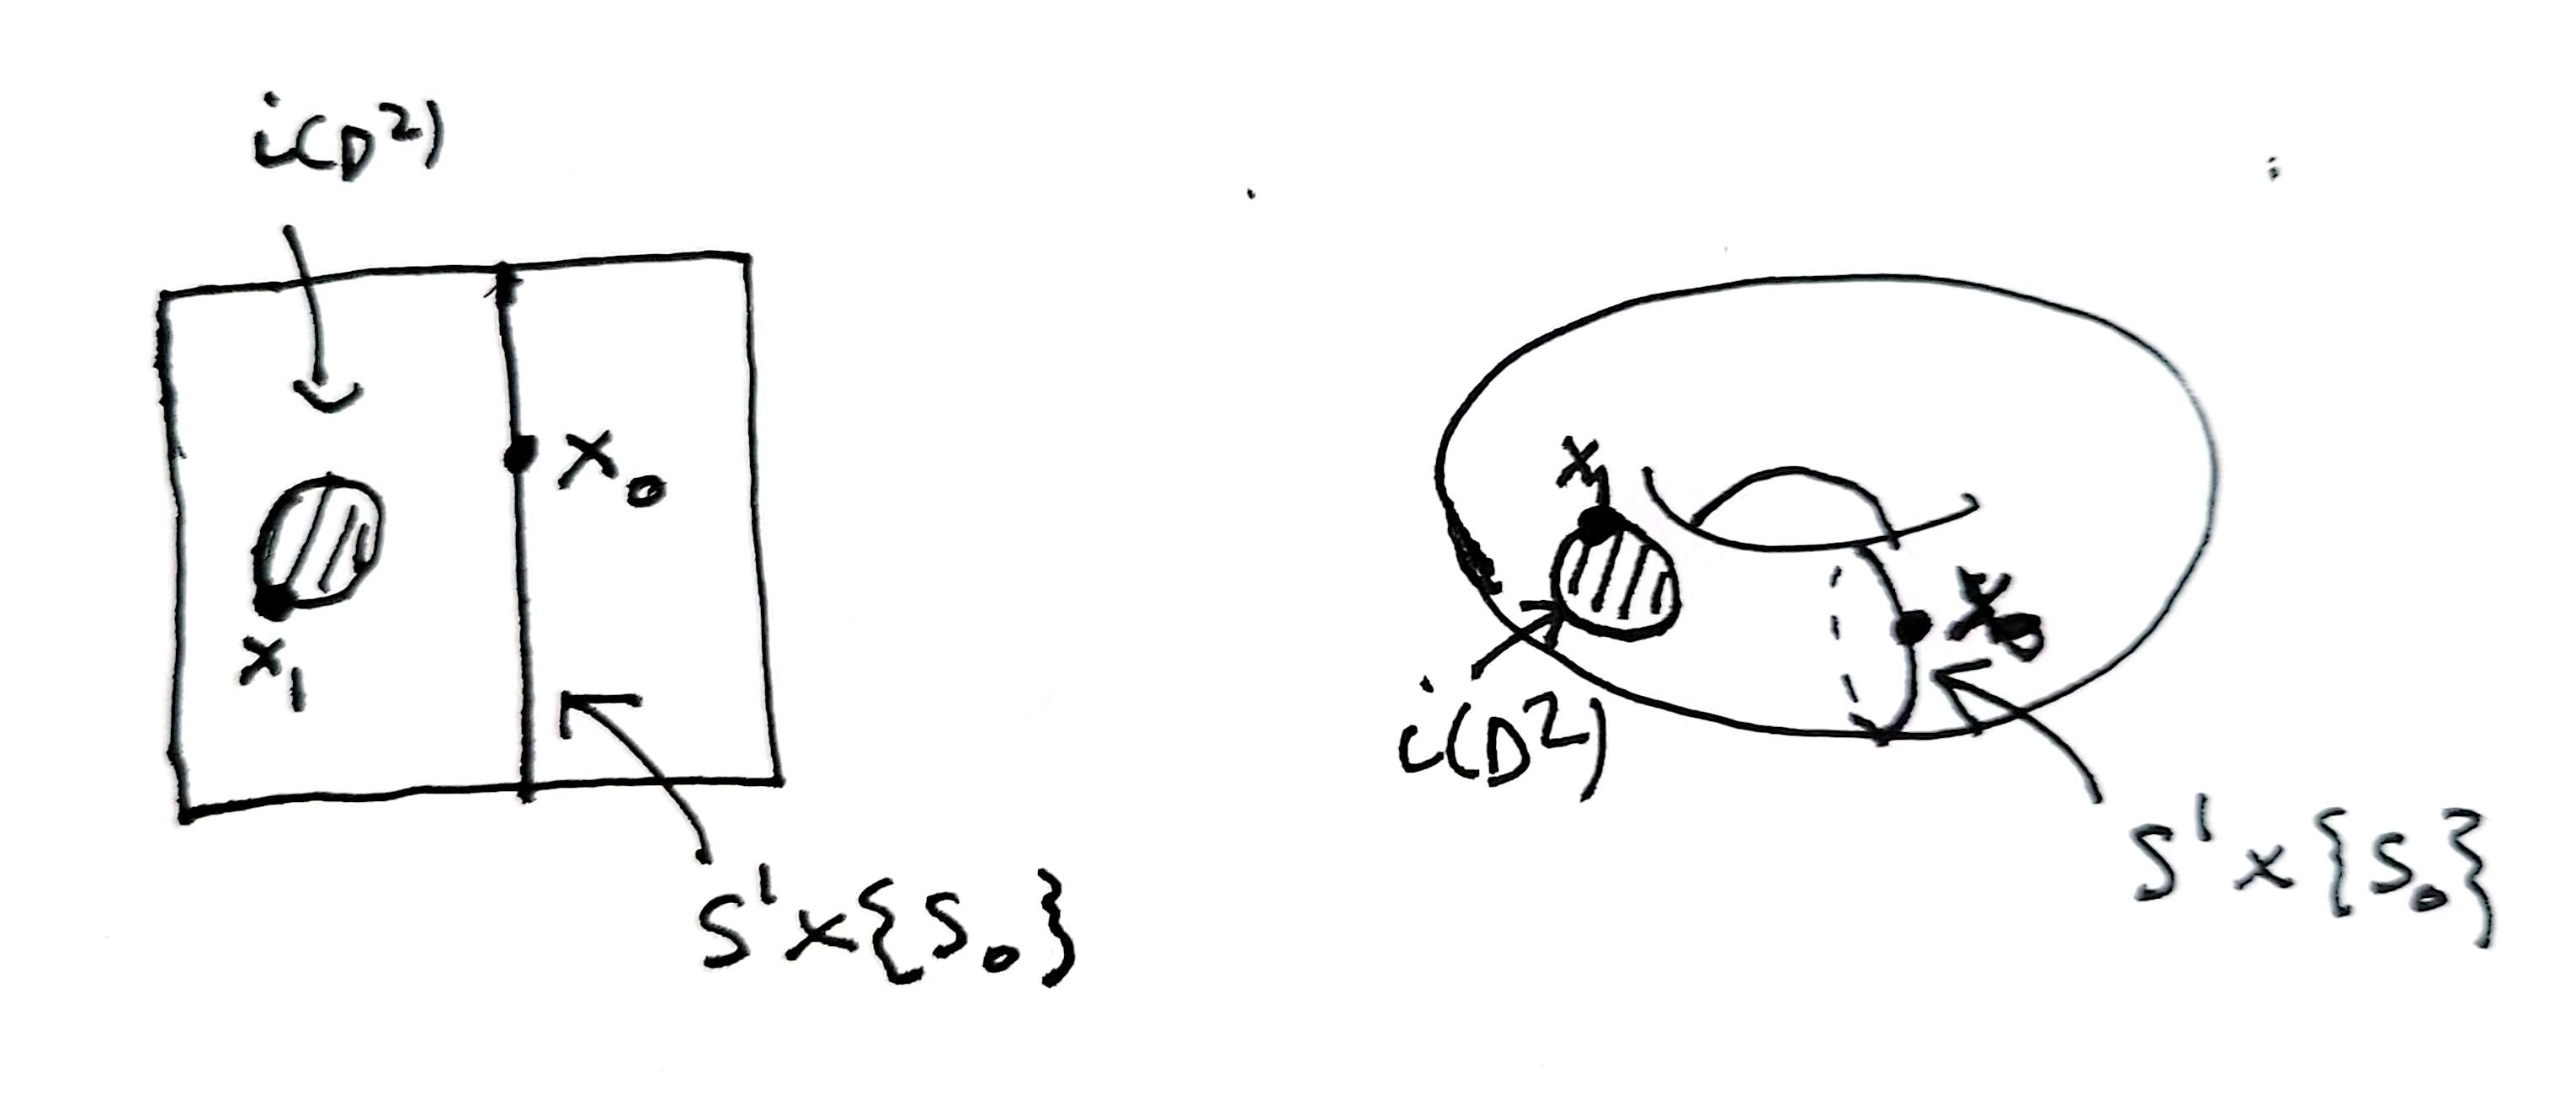
\includegraphics[width=0.8\textwidth]{Figures/p11.jpeg}
            \caption{Note that 
            in this figure, $A$ are the parts drawn
        without the interior of the disk $i(D^2)$.}
            \label{fig:p11-jpeg}
        \end{figure}

        (2)
        Recall that
        \[
        \pi_n (T,A,x_1) =
        \left[ I^{n},\partial I^{n},
        J^{n-1}; T,A, x_1 \right] .
        \] 
        Thus $\pi_1 \left( T,A,x_1 \right) $ becomes
        the set of homotopy classes
        of maps
        $\left( I, \left\{ 0,1 \right\} , \left\{ 1 \right\} 
        \right) \to \left( T,A,x_1 \right)$. That is, the
        set of paths in $T$ starting at a point in $A$ and
        ending at $x_1$ up to homotopy through such paths.\\
        For any map
        $ f \colon \left( I, \left\{ 0 \right\} , \left\{ 1 \right\} 
        \right) \to \left( T, A, \left\{ x_1 \right\}  \right) $, 
        can lift this to the universal cover since
        $I$ is simply connected. Let
        $\tilde{f} \colon 
        \left( I, \left\{ 0 \right\} , \left\{ 1 \right\}  \right) 
        \to \left( \mathbb{R}^2, 
        p^{-1} (A) , p^{-1}\left( \left\{ x_1 \right\}  \right) 
    \right) $.
    Now, $p^{-1}(A)$ can be visualized as
    tiling $\mathbb{R}^2$ by tiles
    as the left picture in Figure \ref{fig:p11-jpeg}, each
    tile of course contains precisely one
    element of the fiber $p^{-1}\left( 
    \left\{ x_1 \right\} \right) $. For the lift
    $\tilde{f}$, we choose a base point
    $\tilde{x_1}$ in
    $p^{-1}\left( \left\{ x_1 \right\}  \right) $. By
    the lifting theorem, there now exists
    a unique lift, call it $\tilde{f} \colon
    \left( I, \left\{ 1 \right\} 
    \right) \to \left( \mathbb{R}^2, 
    \left\{ \tilde{x_1} \right\} \right) $, such that
    $f = p \circ \tilde{f}$. Now,
    $f(0) \in A$ is the only condition, so
    $\tilde{f}(0)$ lies in $p^{-1}(A)$.
    Homotopies through maps which
    start in $A$ for $f$ correspond in the universal cover
    to letting $\tilde{f}(0)$ run freely through its
    path component in $p^{-1}(A)$. We can
    construct a bijection
    $\pi_0 \left( p^{-1}(A) \right) \cong 
    \mathbb{Z}^2 \sqcup \mathbb{Z}$ by
    identifying the component of
    $p^{-1} \left( i \left( S^{1} \right)  \right) \cap
    \left[ n,n+1 \right] \times \left[ m,m+1 \right] $ with
    $\left( n,m \right) \in \mathbb{Z}^2$ and
    identifying the
    vertical line in
    $p^{-1}\left( S^{1} \times \left\{ s_0 \right\}  \right) 
    \cap [n,n+1)$ with $n \in  \mathbb{Z} \subset 
    \mathbb{Z}^2 \sqcup \mathbb{Z}$. This is obviously bijective.
    We can always homotopy $f$ to be a straight-line in
    the universal cover, so the only thing that determines
    the equivalence class of
    $f$, given that $\tilde{f}$ ends at $\tilde{x_1}$,
    is which path component in
    $\mathbb{Z}^2 \sqcup \mathbb{Z}$ it start in.
    This gives an injective map
    $\varphi \colon \pi_1 \left( T,A,x_1 \right) 
    \to \mathbb{Z}^2 \sqcup \mathbb{Z}$.
    To see that it is surjective, it is clear that
    choosing $\tilde{x_1}$ as above and
    choosing any point in the path component corresponding to
    an element $x \in \mathbb{Z}^2 \sqcup \mathbb{Z}$, taking
    the straight line between these two points gives
    a path $\tilde{f} \colon I \to \mathbb{R}^2$ 
    such that $f := p \circ \tilde{f} $ gives a path
    $\left[ f \right] \in \pi_1 \left( T,A,x_1 \right) $,
    and, by construction,
    $\varphi (\left[ f \right] ) = x$.

    Thus $\pi_1 (T,A,x_1) \cong \mathbb{Z}^2 \sqcup \mathbb{Z}$.



        (3) Let
        $\iota \colon A \to T$ be the inclusion.
        Then using the LES of relative homotopy groups, we
        have that 
        \begin{align*}
            \pi_2 (T,x_i)
            \to \pi_2 \left( T,A, x_i \right) 
            \to \pi_1 \left( A,x_i \right) \stackrel{\iota_*}{\to} 
            \pi_1 \left( T,x_i \right) 
        \end{align*}
        is exact for $i = 0,1$.
        For $i=0,1$, 
        $\pi_1 (A,x_i) \cong \mathbb{Z}$ and
        $\pi_1 (T,x_i) \cong \mathbb{Z}^2$, while
        $\pi_2 \left( T,x_i \right) \cong
        \pi_2 \left( S_1 \right) \times 
        \pi_2 \left( S^{1} \right) \cong 1$ for
        both $i=0,1$.
        Hence
        $\pi_2 \left( T,A,x_i \right) \cong
        \ker \iota_*$.
        First, suppose $i = 0$. 
        Then $\iota$ induces the map
        $\mathbb{Z} \cong \pi_1 \left( A, x_0 \right) 
        \to \pi_1 \left( T, x_0 \right) \cong \mathbb{Z}^2$ 
        given by
        $n \mapsto \left( 0,n \right) $, so
        $\ker \iota_*$ is trivial in this case, so
        $\pi_2 \left( T, A, x_0 \right) \cong 0$.
        Suppose now that $i = 1$. Then
        any loop in the image of $\iota_*$ is clearly
        based nullhomotopic by contracting 
        $i(D^2)$ to the point $x_1$. Thus
        $\ker \iota_* =
        \pi_1 \left( A, x_1 \right) 
        \cong \pi_1 (S^{1}) \cong \mathbb{Z}$.
        So $\pi_2 \left( T,A,x_1 \right) \cong
        \mathbb{Z}$.
    \end{solution}


    \begin{problem}[]
        \begin{enumerate}
            \item Compute $\pi_1 \left( S^{1} \vee
                S^2\right) $ and describe the universal
                cover of $S^{1} \vee S^2$.
            \item Show that $\pi_2 \left( S^{1} \vee
                S^2 \right) $ is isomorphic
                to $\bigoplus_{\mathbb{Z}} \mathbb{Z}$.
            \item Explicitly describe the action of
                $\pi_1 \left( S^{1} \vee S^2 \right) $ on
                $\bigoplus_{\mathbb{Z}} \mathbb{Z} \cong
                \pi_2 \left( S^{1} \vee S^2 \right) $.
        \end{enumerate}
    \end{problem}

    \begin{solution}
        (1) 
        The universal cover of $S^{1} \vee S^2 =: X$, which
        we will denote $\tilde{X}$, is
        clearly
        $\mathbb{R}$ with a copy of $S^2$ attached to
        each integer of $\mathbb{R}$.\\
        Let 
        $A_1$ be the $S^{1}$ part
        together with a small open neighborhood
        of the base point in $S^2$, and
        likewise, $A_2$ be $S^2$ together with a small
        open neighborhood of the base point in $S^{1}$ - here
        the base points are the points that get identified
        in the construction of $S^2 \vee S^{1}$.
        Applying van Kampen, we find that
        $\pi_1 \left( S^2 \vee S^{1} \right) 
        \cong \pi_1 \left( S^{1} \right) * \pi_1\left( S^2 \right) 
        / N$ where $N$ is generated
        by all elements of the form
        $i_{12}(w) i_{21}(w)^{-1}$ for
        $w \in \pi_1 \left( A_1 \cap A_2 \right) $.
        But $A_1 \cap A_2$ is contractible, so
        $N \cong 0$. Since $\pi_1 \left( S^{1} \right) \cong
        \mathbb{Z}$ and $\pi_1 \left( S^2 \right) \cong 0$, 
        we conclude that $\pi_1 \left( S^{2} \vee S^{1}  \right) 
        \cong \mathbb{Z}$.\\
        \linebreak
        (2) To compute
        $\pi_2 \left( S^{1} \vee S^2 \right) $, it suffices
        to compute $\pi_2$ of its universal cover since
        these are isomorphic. The universal cover
        is $\mathbb{R}$ with $S^2$ attached at each integer.
        Since $\mathbb{R} \simeq \left\{ * \right\}$, the
        universal cover is homotopy equivalent to
        $\vee_{\mathbb{Z}} S^2$ for example by
        using proposition 0.16 and 0.17 in Hatcher.\\
        Since homotopy groups are invariant under based homotopy
        equivalences, it suffices to
        compute $\pi_2 \left( \bigvee_{\mathbb{Z}}S^{2} \right) $.\\
        But $\bigvee_{\mathbb{Z}}S^2$ is $1$-connected,
        so if $\tilde{H}_2 \left( \bigvee_{\mathbb{Z}}S^2 \right) 
        \cong H_2 \left( \bigvee_{\mathbb{Z}}S^2 \right) $ 
        is nonzero, then by the Hurewicz theorem,
        we will obtain that 
        $\pi_2\left( \bigvee_{\mathbb{Z}}S^2 \right) 
        \cong H_2 \left( \bigvee_{\mathbb{Z}}S^2 \right) $.
        Now, we can give
        $\bigvee_{\mathbb{Z}}S^2$ a $\Delta$-complex (or
        cellular) structure
        with a single $0$-simplex
        and a $2$-simplex for each
        $S^2$ in $\bigvee_{\mathbb{Z}}S^2$. The
        associated simplicial chain complex then becomes
        \[
        \ldots \to 0 \to \bigoplus_{\mathbb{Z}}\mathbb{Z}
        \to 0 \to \mathbb{Z} \to 0 \to \ldots
        \] 
        with $0$ everywhere else. In particular then
        $H_2 \left( \bigvee_{\mathbb{Z}}S^2 \right) 
        \cong \oplus_{\mathbb{Z}}\mathbb{Z}$ since there
        cannot be any cancellation from the
        maps.
        Since the Hurewicz isomorphism 
        takes 
        $f \in \pi_2 \left( \bigvee_{\mathbb{Z}} S^2 \right) $,
        to $f_* \left[ 1 \right] \in 
        H_2 \left( \bigvee_{\mathbb{Z}}S^2 \right) $ 
        for $\left[ 1 \right] \in H_2\left( S^2 \right) $ 
        a generator, we find that through our proof
        using the $\Delta$-complex of $\bigvee_{\mathbb{Z}}S^2$,
        we found that the inclusions
        $S^2 \hookrightarrow \bigvee_{\mathbb{Z}}S^2$ 
        in fact induce generators on homology: i.e.,
        the images of the different inclusions
        $\iota_i \colon H_2 \left( S_i^2 \right) 
        \hookrightarrow H_2 \left( \bigvee_{i \in \mathbb{Z}}
        S_i^2 \right) 
        \cong \bigoplus_{\mathbb{Z}}\mathbb{Z}$ generate
        $\bigoplus_{\mathbb{Z}} \mathbb{Z}$, and hence
        also $\pi_2 \left( \bigvee_{\mathbb{Z}}S^2 \right) $ 
        under the Hurewicz isomorphism.\\
        \linebreak
        








    (3) 
    Recall that
    the action of $\pi_1 \left( S^{1} \vee S^2 \right) $ 
    on $\pi_n \left( S^{1} \vee S^{2} \right) $ 
    makes $\pi_n \left( S^{1} \vee S^2 \right) $ 
    into a $\mathbb{Z} \left[ \pi_1 \left( S^{1} \vee S^2 \right) 
    \right] $-module. We saw that
    $\pi_1 \left( S^{1} \vee S^2 \right) \cong \mathbb{Z}$. Let
    $\gamma$ be a loop that goes once around the $S^{1}$ factor.
    This generates $\pi_1 \left( S^{1} \vee S^2 \right) 
    \cong \mathbb{Z}$, so it suffices
    to describe the action of $\gamma$ on
    $\pi_2 \left( S^{1} \vee S^2 \right) $ since
    $\pi_2$ now becomes a $\mathbb{Z}\left[ \gamma \right] $-module
    under this action.
    Since also $\pi_2 \left( S^{1} \vee S^2 \right) 
    \cong \bigoplus_{\mathbb{Z}} \mathbb{Z}$, it
    suffices to describe the action of
    $\gamma$ on an arbitrary basis element
    of $\bigoplus_{\mathbb{Z}}\mathbb{Z}$, say,
    corresponding to the image under $p_*$ of
    some an inclusion of some $S^2 \hookrightarrow 
    \tilde{X}$. Suppose we choose the inclusion
    $\alpha$ into the $S^2$ attached to $1_n \in \mathbb{Z}_n$.\\
    Then $p_* \alpha = \left[ \eta_n \xi \right]
    = 1_{n} \in \mathbb{Z}_n$ where
    $\eta_n$ is the loop that winds around the $S^{1}$ factor
    $n$ times and $\xi$ is the inclusion
    $S^2 \hookrightarrow S^{1} \vee S^2$.\\
    In particular then
    $\gamma p_* \alpha = \left[ \eta_{n+1} \xi \right] 
    = 1_{n+1} \in \mathbb{Z}_{n+1}$.\\
    \linebreak
    This completes the description, but I will also
    give an alternative description just for
    completeness where I expound on some details
    between the homomorphisms
    $H_2 \left( \bigvee_{\mathbb{Z}}S^2 \right) 
    \cong \pi_2 \left( \bigvee_{\mathbb{Z}} S^2 \right) 
    \cong \pi_2 \left( S^{1} \vee S^2 \right) $ that underlies
    the above explanation. We will use the correspondence between
    the $\pi_1$ action on $\pi_n (X)$ and its action
    on $\pi_n \left( \tilde{X} \right)  $ where
    $\tilde{X}$ was the universal covering space.\\
    To this end, we have previously shown the following:
    \begin{lemma}[]
        Let $p \colon \tilde{X} \to X$ be the universal cover
        of a path-connected space $X$. Under
        the isomorphism $\pi_n (X) \cong \pi_n (\tilde{X})$, for
        $n\ge 2$, the action of $\pi_1 (X)$ on
        $\pi_n (X)$ corresponds to the action
        of $\pi_1(X)$ on $\pi_n \left( \tilde{X} \right) $ 
        induced by the action of $\pi_1 (X)$ on
        $\tilde{X}$ as deck transformations.
        More precisely,
        for $\gamma \in \pi_1 \left( X, x_0 \right) ,
        \alpha \in \pi_n \left( \tilde{X},
        \tilde{x}_0 \right) ,
        \tilde{\gamma}$  the lift of $\gamma$, and
        $\gamma_*$ the homomorphism induced
        by the action of $\gamma$ on $\tilde{X}$, we have
        $\gamma p_* \left( \alpha \right) =
        p_* \left( \beta_{\tilde{\gamma}} 
        \left( \gamma_* \left( \alpha \right)  \right) \right) $.
    \end{lemma}

    Let $\alpha \in \pi_2 \left( \tilde{X} \right) $  be
    the element corresponding under the isomorphism
    $\pi_2 (X) \cong \pi_2(\tilde{X})$ to the class
    of our chosen
    inclusion $S^2 \hookrightarrow \bigvee_{\mathbb{Z}}S^2$.
    That is, $\alpha$ is the inclusion of
    $S^2$ into one of the $S^2$ in the universal cover.
    To understand $\gamma p_* \left( \alpha \right) $, we
    can thus look at
    $p_* \left( \beta_{\tilde{\gamma}} 
    \left( \gamma_* \left( \alpha \right)  \right) \right) $.
    Now, $\gamma_* \left( \alpha \right) $ will
    simply be the inclusion of $S^2$ to 
    the $S^2$ "above" the previous one in the
    universal cover. So if we previously included our
    $S^2$ into the $S^2$ attached to
    $n \in \mathbb{R} \subset \tilde{X}$, then
    $\gamma_* \left( \alpha \right) $ corresponds to
    including $S^2$ into the $S^2$ attached to
    $n+1 \in \mathbb{R} \subset \tilde{X}$.
    Then $\beta_{\tilde{\gamma}}$ is simply the change-or-basepoint
    transformation depicted in the picture on
    page 341 in Hatcher. I.e., it essentially shrinks
    $\alpha$ and attaches it inside a larger square
    where we put $\tilde{\gamma}$ on each radial line
    in-between  the squares. 
    If we understand our isomorphism
    $\pi_2 \left( \bigvee_{\mathbb{Z}}S^2 \right) 
    \cong \bigoplus_{i \in \mathbb{Z}}\mathbb{Z}_i$ as
    the generator for $\mathbb{Z}_i$ corresponding under
    the Hurewicz isomorphism to the inclusion
    of $S^2$ into the sphere attached to $i \in \mathbb{Z}$,
    then we find that
    $\alpha \mapsto 
    \beta_{\tilde{\gamma}} \left( \gamma_* \left( \alpha \right) 
    \right) $ precisely sends $\alpha = 
    1_n \in \mathbb{Z}_n$ to $1_{n+1} \in \mathbb{Z}_{n+1}$. 
    Under $p_*$, this
    may be interpreted again as
    sending $1_{n} \mapsto 1_{n+1}$ when
    $n$ corresponds to $ \left[ \eta
    \xi \right]$ where
    $\eta$ is the loop that winds around the $S^{1}$ factor
    $n$ times and
    $\xi$ is the inclusion of $S^2 \hookrightarrow
    S^{1} \vee S^2$.
    \end{solution}


    \begin{problem}[]
        Let $\left( X,A,x_0 \right) $ be a pointed pair
        such that the inclusion
        $i \colon A \hookrightarrow X$ is based nullhomotopic
        (the nullhomotopy preserves the basepoint). The goal
        is to show that for $n\ge 2$, there is an isomorphism
        of groups:
        \[
        \pi_n (X,A,x_0) \cong \pi_n (X,x_0) \times 
        \pi_{n-1}(A,x_0).
        \] 
        \begin{enumerate}
            \item Show that there is an exact sequence
                of groups
                \[
                1 \to \pi_n (X,x_0) 
                \stackrel{j_*}{\to} 
                \pi_n \left( X, A, x_0 \right) 
                \stackrel{\partial_*}{\to} 
                \pi_{n-1}(A,x_0) \to 1.
                \] 
            \item Using a based nullhomotopy
                $H \colon A \times \left[ 0,1 \right] 
                \to X$, construct a natural group morphism
                \[
                r_* \colon \pi_n (X,A,x_0) \to 
                \pi_n (X,x_0)
                \] 
                such that $r_* \circ j_* = 1$.
            \item Show that for any short exact sequence
                of groups
                \[
                1 \to A \stackrel{\alpha}{\to} 
                B \stackrel{\beta}{\to} C \to 1
                \] 
                such that $\alpha$ admits a retraction, there
                is a group isomorphism
                \[
                B \cong A \times C.
                \] 
                Conclude the desired isomorphism.
        \end{enumerate}
    \end{problem}

    \begin{proof}
        (1) From the LES for relative homotopy groups, we obtain that
        \[
        \pi_n (A, x_0) \stackrel{i_*}{\to}  \pi_n(X,x_0)
        \stackrel{j_*}{\to} \pi_n \left( X, A, x_0 \right) 
        \stackrel{\partial_*}{\to} 
        \pi_{n-1}(A,x_0) \stackrel{i_*}{\to} 
        \pi_{n-1} \left( X, x_0 \right) 
        \] 
        is exact.
        For $n\ge 2$, all the sets in the exact sequence are
        groups and the maps are group homomorphisms.
        Since homotopic maps relative to the base point induce
        the same maps on homotopy groups, we find by assumption
        that $i_* = 0$. Therefore,
        \[
        1 \stackrel{0}{\to}   \pi_n(X,x_0)
        \stackrel{j_*}{\to} \pi_n \left( X, A, x_0 \right) 
        \stackrel{\partial_*}{\to} 
        \pi_{n-1}(A,x_0) \stackrel{0}{\to} 
        1
        \] 
        is exact.\\
        \linebreak
        (2) Let
        $\left[ f \right] \in \pi_n \left( X, A,x_0 \right) $
        and consider a representative
        $f \colon \left( D^{n}, S^{n-1},
        s_0 \right) \to 
        \left( X,A,x_0 \right) $.
        We put $f$ on the bottom of a cylinder
        $D^{n} \times \left\{ 0 \right\} \subset 
        D^{n} \times I$.
        Now $H \left( f(x),t \right) $ 
        gives a homotopy
        $S^{n-1} \times I \to X$, so we
        can use this on 
        $S^{n-1} \times I \subset 
        D^{n} \times I$ of the cylinder.
        Now we use that
        $D^{n} \times \left\{ 0 \right\} 
        \cup S^{n-1} \times I \cong
        D^{n}$ (see Figure \ref{fig:p31-jpeg}). 
        Denote this
        homeomorphism by $\varphi 
        \colon D^{n} \to D^{n} \times \left\{ 0 \right\} \cup 
        S^{n-1} \times I$.

        \begin{figure}[htpb]
            \centering
            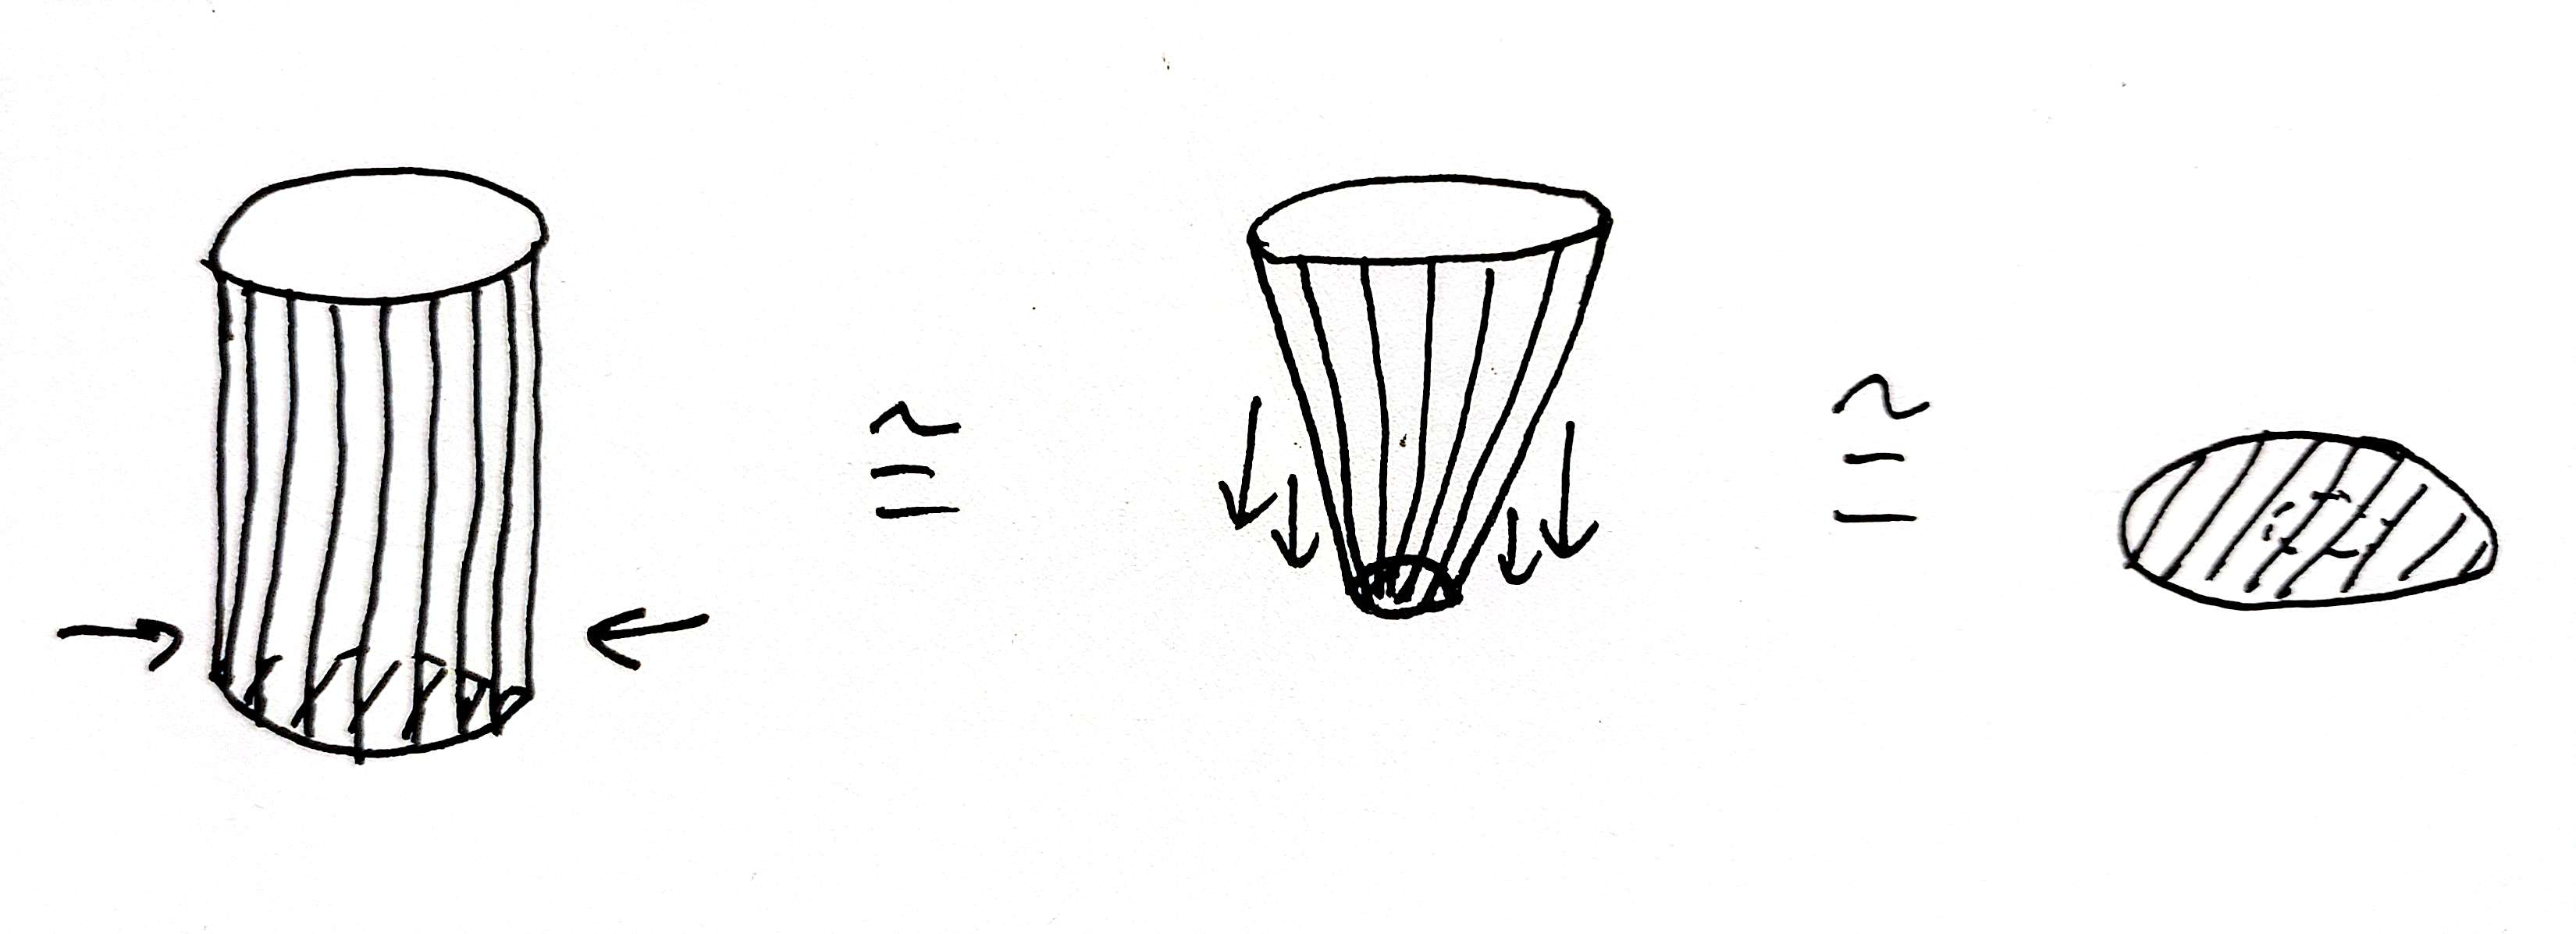
\includegraphics[width=0.8\textwidth]{Figures/p31.jpeg}
            \caption{}
            \label{fig:p31-jpeg}
        \end{figure}

        Define
        $h \colon S^{n-1} \times I$ by
        $h(x,t ) = H\left( f(x), t \right) $ and
        define $h \cup f \colon
        D^{n} \times \left\{ 0 \right\} \cup 
        S^{n-1} \times I$ by
        $f$ on $D^{n} \times \left\{ 0 \right\} $ and
        $h$ on $S^{n-1} \times I$. Then define
        $h \cup f \circ \varphi \colon
        D^{n} \to X$.
        Now $h \cup f \circ \varphi $ maps
        $\partial D^{n}$ to
        $x_0$, so
        it factors through the quotient
        $D^{n} \to S^{n}$ and induces
        a map
        $ \Gamma
        \colon \left( S^{n}, pt \right) 
        \to \left( X,x_0 \right) $, where
        $pt$ is the point that the boundary collapses to.
        This is well-defined since if
        $f \simeq f' \rel s_0$ through 
        a homotopy $F \colon D^{n} \times I \to X$, then
        $\tilde{h}(x,t,s) = 
        H\left( F(x,s), t \right) $ gives a map
        $S^{n-1} \times I \times I$ - and
        this homotopy is constant on the
        boundary $S^{n-1} \times \left\{ 1 \right\} $.
        Then taking
        $\tilde{h} \cup  F \colon
        \left( D^{n} \times \left\{ 0 \right\} 
        \cup S^{n-1} \times I\right)  \times I 
        \cong D^{n-1} \times \left\{ 0 \right\} \times I
        \cup S^{n-1} \times I \times I \to X$, we
        obtain a homotopy
        $\tilde{h}\cup F \circ \varphi \colon
        D^{n} \times I \to X$ which is constant on the
        boundary throughout, hence induces the desired
        homotopy $S^{n} \times I \to X$ between
        $\Gamma$ and $\Gamma' \rel \left\{ pt \right\} $.\\
        To see that it is a group morphism,
        see Figure \ref{fig:p32-jpeg}. Here
        the top left picture depicts
        $\Gamma$ obtained from
        $f + g \in 
        \pi_n \left( X, A, x_0 \right) $.
        The bottom left picture represents
        $\Gamma_f + \Gamma_g$, where
        $\Gamma_f$ is obtained from $f$ by the above procedure
        and $\Gamma_g$ is obtained from
        $g$ by the procedure. 
        Hence $r_* \left( \left[ f \right] +
        \left[ g \right] \right) 
        = r_* \left( \left[ f \right]  \right) 
        + r_* \left( \left[ g \right]  \right) $.

        \begin{figure}[htpb]
            \centering
            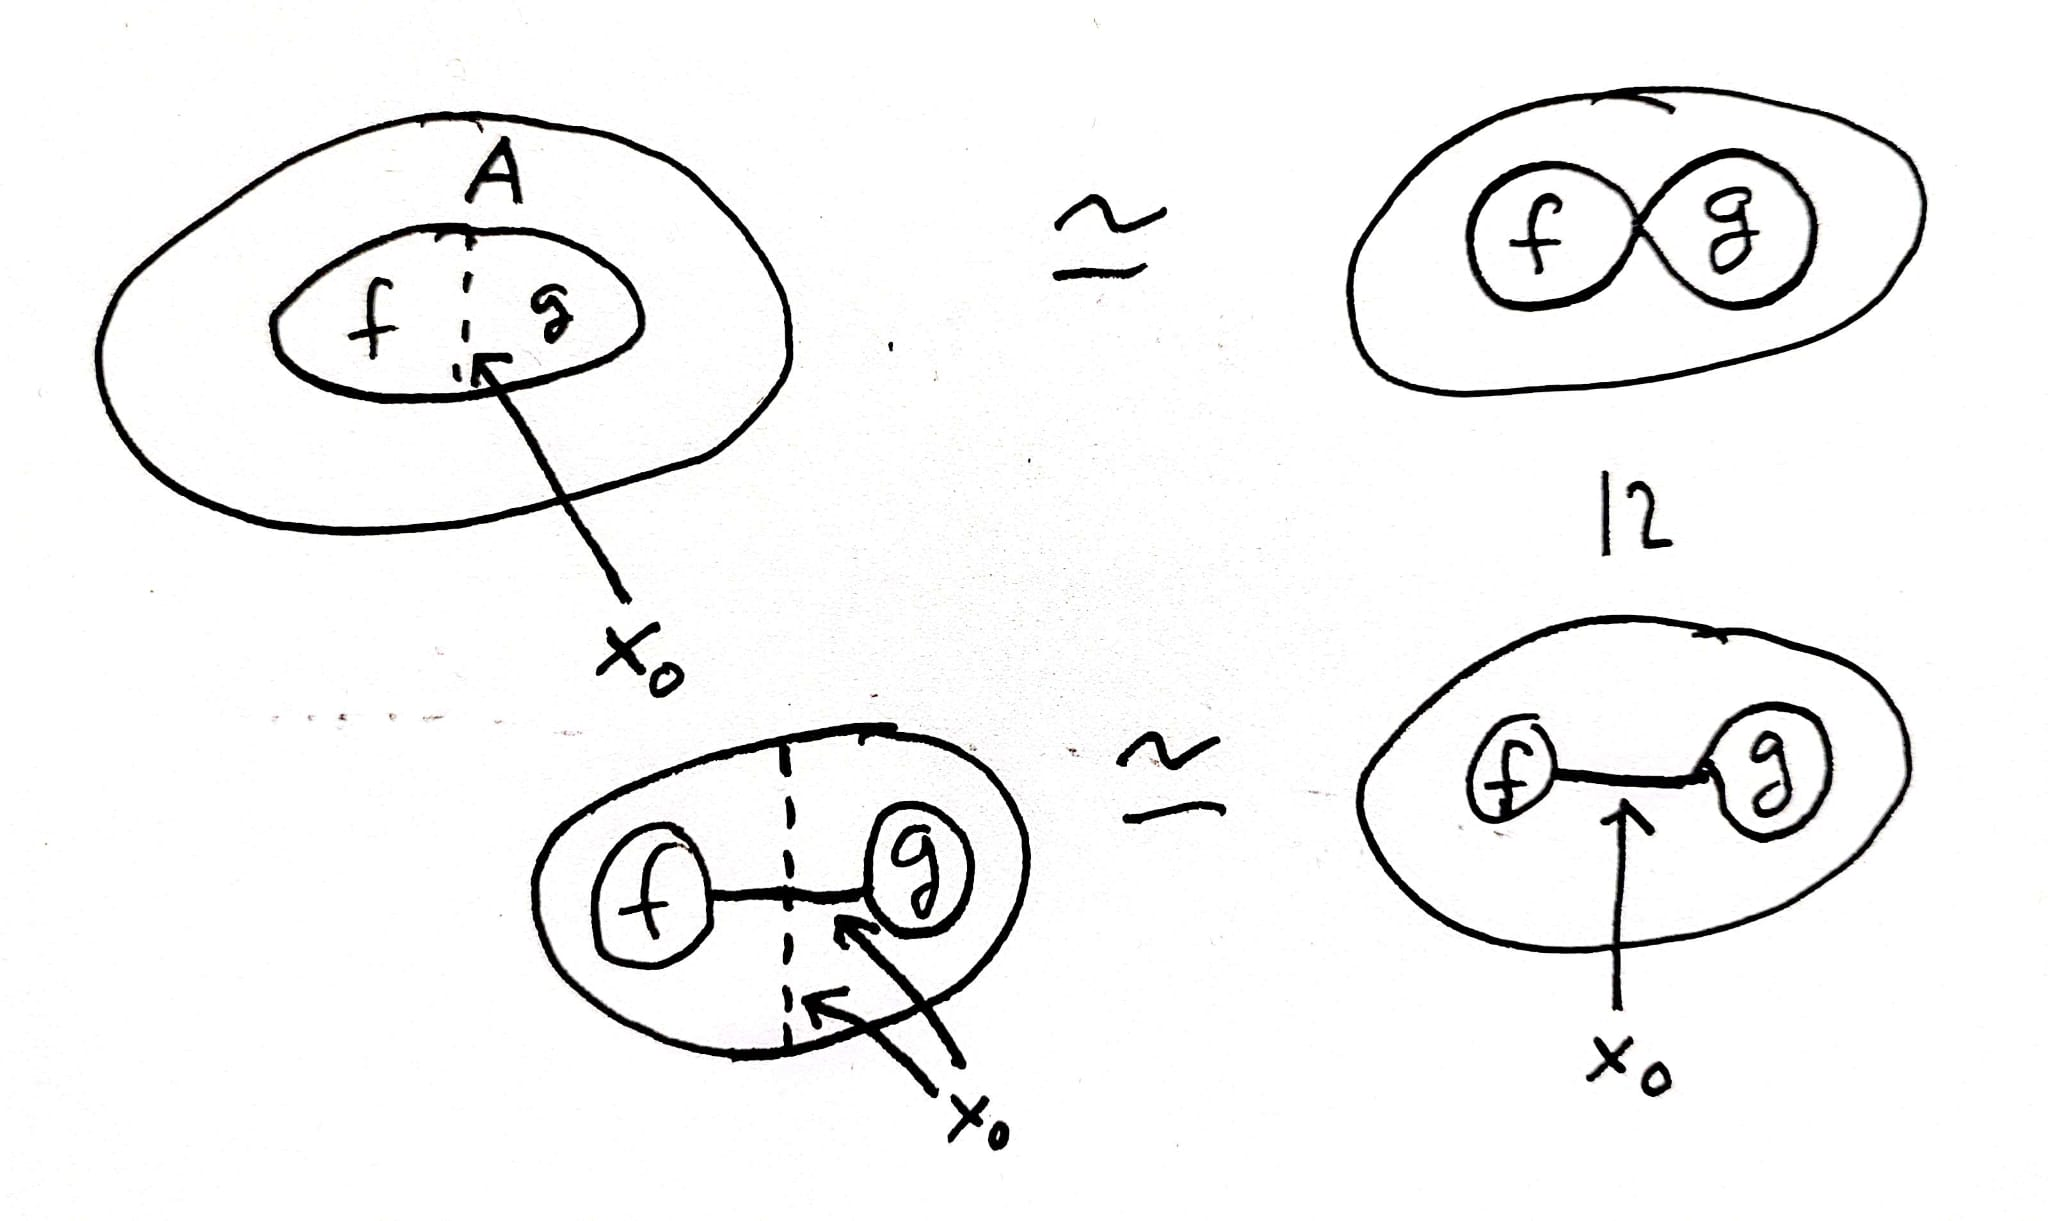
\includegraphics[width=0.7\textwidth]{Figures/p32.jpeg}
            \caption{}
            \label{fig:p32-jpeg}
        \end{figure}

        Naturality amounts to showing that 
        $r_*$ defines a natural transformation from
        $\pi_n \left( - , -, - \right) $ to
        $\pi_n (-,-)$ on the
        category of based pairs $\left( X,A \right) $ 
        such that $A \hookrightarrow X$ is
        based nullhomotopic. That is, that given
        a map  $f \colon \left( X, A, x_0 \right) 
        \to \left( Y,B,y_0 \right) $, with
        both $A \hookrightarrow X$ and
        $B \hookrightarrow Y$ based nullhomotopic, the diagram
        \begin{equation*}
        \begin{tikzcd}
            \pi_n \left( X,A,x_0 \right) \ar[r, "r_*"] \ar[d, "
            f_*"] &
            \pi_n (X,x_0) \ar[d, "f_*"] \\
            \pi_n \left( Y,B,y_0 \right) \ar[r, "r_*"] & 
            \pi_n (Y,y_0)
        \end{tikzcd}
        \end{equation*}
        commutes.

        Now, if $H \colon A \times I \to X$ is
        the based nullhomotopy
        of $A \hookrightarrow X$ and
        $G \colon B \times I \to Y$ is the based
        nullhomotopy of 
        $B \hookrightarrow Y$, then
        for $\left[ f \right] \in 
        \pi_n \left( X,A,x_0 \right) $, we get the
        situation of
        Figure \ref{fig:p33-jpeg}.
        In the central part, these maps agree - namely they
        are $f \circ g$. We are thus asking for
        a homotopy
        between
        $f \circ H \left( g(x),t \right) $ and
        $G\left( f \circ g(x), t \right) $. So
         we want a map
         $L \colon S^{n-1} \times I \times I \to X$. 
         We may assume without loss of generality
         that $H$ and $G$ map
         $S^{n-1} \times \left\{ 0 \right\} $ to
         $x_0$ and $y_0$, respectively, instead
         of $S^{n-1} \times \left\{ 1 \right\} $.
         Now we let $L$ be
         given by
         \[
         L \left( x, t, s \right) 
         \begin{cases}
             f \circ H\left( g(x), (1-2s) t \right) ,& 
             s \in \left[ 0,\frac{1}{2} \right] \\
             G \left( f \circ g(x), 2s-1 \right),& s 
             \in \left[ \frac{1}{2},1 \right].
         \end{cases}
         \] 
         This gives naturality.

        \begin{figure}[htpb]
            \centering
            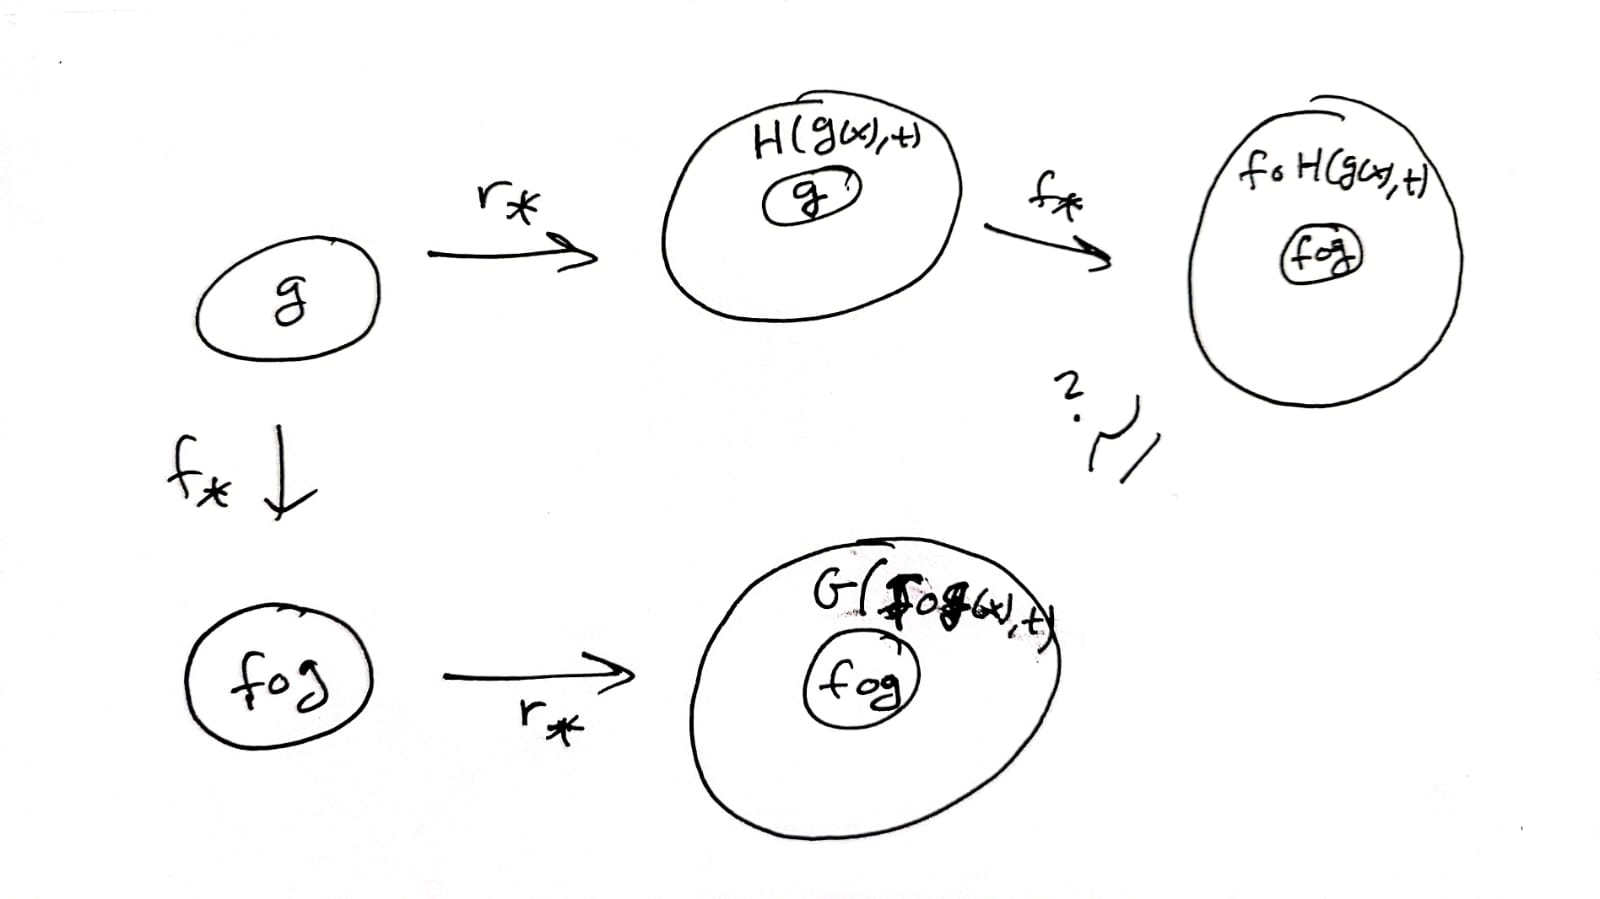
\includegraphics[width=0.8\textwidth]{Figures/p33.jpeg}
            \caption{}
            \label{fig:p33-jpeg}
        \end{figure}
        





        Now, for 
        $\left[ f \right]  \in \pi_n \left( X, x_0 \right) $,
        we have that the boundary is
        already mapped to $x_0$, so
        $H \left( f(x), t \right)$ is constant
        on $S^{n-1} \times I$ since
        $H$ is relative the basepoint. Hence
        $\Gamma \simeq f$ as depicted in
        Figure \ref{fig:p322-jpeg} where
        $\Gamma$ is obtained from
        $j_* \left[ f \right] $ which is simply 
        $\left[ f \right] \in 
        \pi_n \left( X,A,x_0 \right) $.

        \begin{figure}[htpb]
            \centering
            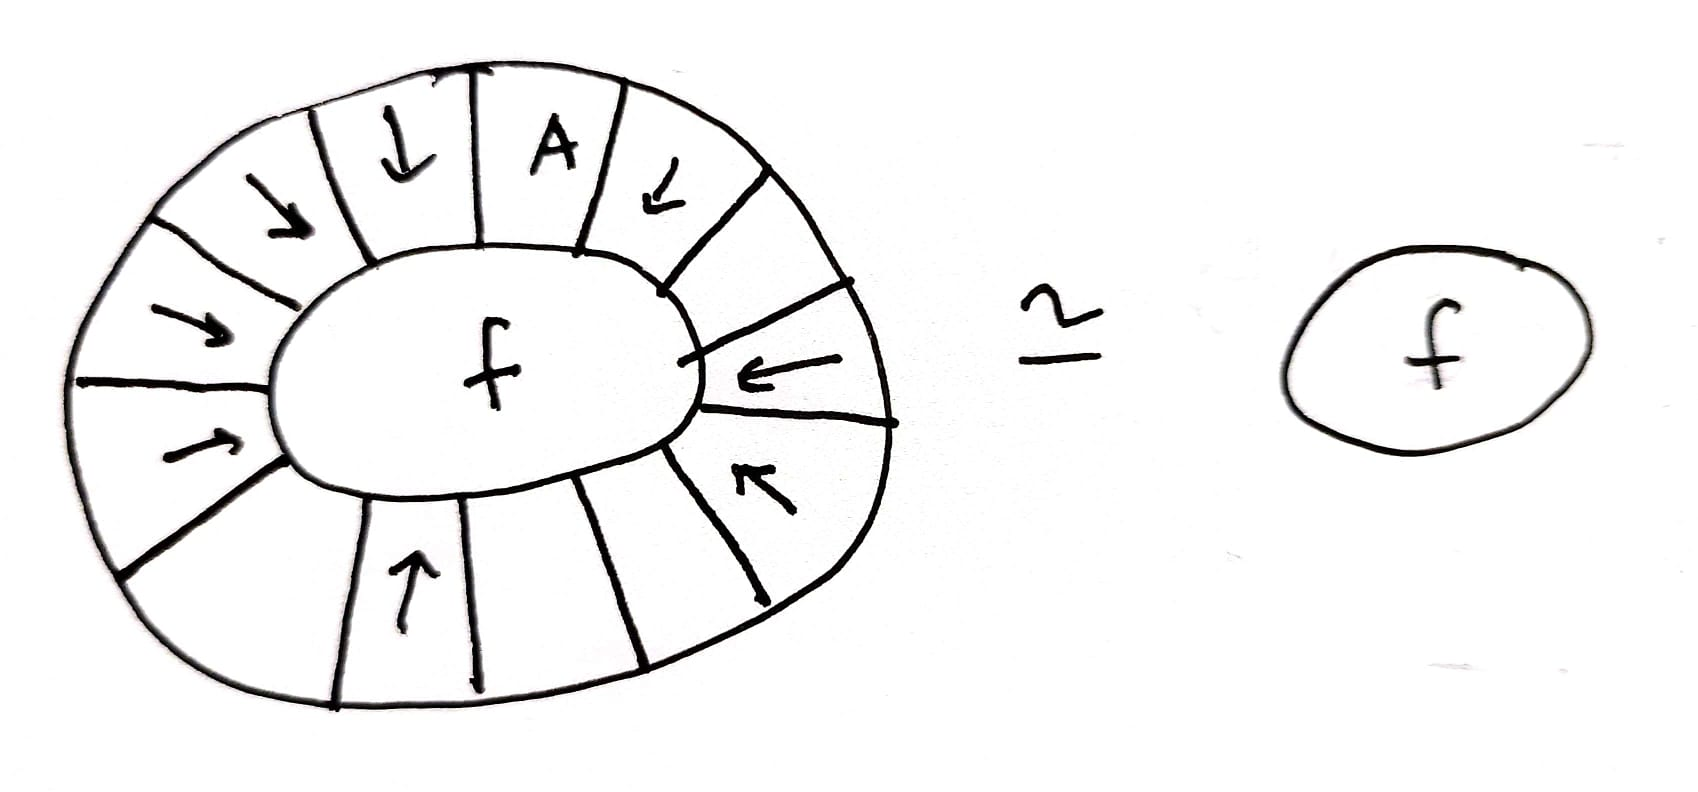
\includegraphics[width=0.6\textwidth]{Figures/p322.jpeg}
            \caption{}
            \label{fig:p322-jpeg}
        \end{figure}
        
        This shows that
        $r_* \circ j_* = \id$ which was what we wanted to show.\\
        \linebreak
        (3) Suppose
        \[
        1 \to A \stackrel{\alpha}{\to} B
        \stackrel{\beta}{\to} C \to 1
        \] 
        is a short exact sequence and
        let $s \colon B \to A$ be a retraction - i.e.,
        $s \circ \alpha = \id$.
        We claim that
        $\varphi \colon B \to A \times C$ by
        $\varphi (b) = \left( s(b),
        \beta(b)\right) $ is an isomorphism.
        Firstly, it is clearly a group homomorphism
        since $s$ and $\beta$ are assumed to be group homomorphisms.
        Next, for injectivity,
        if $\varphi (b) = 0$, then
        $s(b) = 0$ and $\beta(b) = 0$. But
        by exactness then there exists
        $a \in A$ such that $\alpha(a) = b$.
        Thus
        $a = \id (a)  = s \circ \alpha(a) 
        = s (b) = 0$. But then since
        $\alpha$ is a group homomorphism, it takes
        $0$ to $0$, so
        $b = \alpha(a) = \alpha(0) = 0$. This gives
        injectivity.\\
        For surjectivity, let
        $\left( a,c \right) \in A \times C$.
        Since $\beta$ is surjective by exactness of the SES,
        there exists $b \in B$ such that
        $\beta (b) = c$. Then
        $s (\alpha(a) - \alpha \circ s(b) +  b) =
        a - s(b) + s(b) = a$ while
        $\beta \left( \alpha(a) -
        \alpha \circ s(b) + b\right) 
        = \beta(b) = c$ since
        $\beta \circ \alpha = 0$. Hence
        $\varphi \left( \alpha(a - s(b))
         + b\right) = \left( a,c \right) $, so
         $\varphi $ is also surjective.\\
         To conclude the desired isomorphism of
         the problem, we simply note that
         by (1) and (2), we precisely have
         an exact sequence where
         $j_*$ admits a retraction, so
         by (3), we get an isomorphism
         \[
         \pi_n \left( X,A,x_0 \right) 
         \cong \pi_n (X,x_0) \times 
         \pi_{n-1}(A,x_0).
         \] 
    \end{proof}





%\documentclass[reqno]{amsart}
\usepackage{amscd, amssymb, amsmath, amsthm}
\usepackage{graphicx}
\usepackage[colorlinks=true,linkcolor=blue]{hyperref}
\usepackage[utf8]{inputenc}
\usepackage[T1]{fontenc}
\usepackage{textcomp}
\usepackage{babel}
%% for identity function 1:
\usepackage{bbm}
%%For category theory diagrams:
\usepackage{tikz-cd}

%\usepackage[backend=biber]{biblatex}
%\addbibresource{.bib}


\setlength\parindent{0pt}

\pdfsuppresswarningpagegroup=1

\newtheorem{theorem}{Theorem}[section]
\newtheorem{lemma}[theorem]{Lemma}
\newtheorem{proposition}[theorem]{Proposition}
\newtheorem{corollary}[theorem]{Corollary}
\newtheorem{conjecture}[theorem]{Conjecture}

\theoremstyle{definition}
\newtheorem{definition}[theorem]{Definition}
\newtheorem{example}[theorem]{Example}
\newtheorem{exercise}[theorem]{Exercise}
\newtheorem{problem}[theorem]{Problem}
\newtheorem{question}[theorem]{Question}

\theoremstyle{remark}
\newtheorem*{remark}{Remark}
\newtheorem*{note}{Note}
\newtheorem*{solution}{Solution}



%Inequalities
\newcommand{\cycsum}{\sum_{\mathrm{cyc}}}
\newcommand{\symsum}{\sum_{\mathrm{sym}}}
\newcommand{\cycprod}{\prod_{\mathrm{cyc}}}
\newcommand{\symprod}{\prod_{\mathrm{sym}}}

%Linear Algebra

\DeclareMathOperator{\Span}{span}
\DeclareMathOperator{\im}{im}
\DeclareMathOperator{\diag}{diag}
\DeclareMathOperator{\Ker}{Ker}
\DeclareMathOperator{\ob}{ob}
\DeclareMathOperator{\Hom}{Hom}
\DeclareMathOperator{\Mor}{Mor}
\DeclareMathOperator{\sk}{sk}
\DeclareMathOperator{\Vect}{Vect}
\DeclareMathOperator{\Set}{Set}
\DeclareMathOperator{\Group}{Group}
\DeclareMathOperator{\Ring}{Ring}
\DeclareMathOperator{\Ab}{Ab}
\DeclareMathOperator{\Top}{Top}
\DeclareMathOperator{\hTop}{hTop}
\DeclareMathOperator{\Htpy}{Htpy}
\DeclareMathOperator{\Cat}{Cat}
\DeclareMathOperator{\CAT}{CAT}
\DeclareMathOperator{\Cone}{Cone}
\DeclareMathOperator{\dom}{dom}
\DeclareMathOperator{\cod}{cod}
\DeclareMathOperator{\Aut}{Aut}
\DeclareMathOperator{\Mat}{Mat}
\DeclareMathOperator{\Fin}{Fin}
\DeclareMathOperator{\rel}{rel}
\DeclareMathOperator{\Int}{Int}
\DeclareMathOperator{\sgn}{sgn}
\DeclareMathOperator{\Homeo}{Homeo}
\DeclareMathOperator{\SHomeo}{SHomeo}
\DeclareMathOperator{\PSL}{PSL}
\DeclareMathOperator{\Bil}{Bil}
\DeclareMathOperator{\Sym}{Sym}
\DeclareMathOperator{\Skew}{Skew}
\DeclareMathOperator{\Alt}{Alt}
\DeclareMathOperator{\Quad}{Quad}
\DeclareMathOperator{\Sin}{Sin}
\DeclareMathOperator{\Supp}{Supp}
\DeclareMathOperator{\Char}{char}
\DeclareMathOperator{\Teich}{Teich}
\DeclareMathOperator{\GL}{GL}
\DeclareMathOperator{\tr}{tr}
\DeclareMathOperator{\codim}{codim}
\DeclareMathOperator{\coker}{coker}
\DeclareMathOperator{\corank}{corank}
\DeclareMathOperator{\rank}{rank}
\DeclareMathOperator{\Diff}{Diff}
\DeclareMathOperator{\Bun}{Bun}
\DeclareMathOperator{\Sm}{Sm}
\DeclareMathOperator{\Fr}{Fr}
\DeclareMathOperator{\Cob}{Cob}
\DeclareMathOperator{\Ext}{Ext}
\DeclareMathOperator{\Tor}{Tor}
\DeclareMathOperator{\colim}{colim}



%Row operations
\newcommand{\elem}[1]{% elementary operations
\xrightarrow{\substack{#1}}%
}

\newcommand{\lelem}[1]{% elementary operations (left alignment)
\xrightarrow{\begin{subarray}{l}#1\end{subarray}}%
}

%SS
\DeclareMathOperator{\supp}{supp}
\DeclareMathOperator{\Var}{Var}

%NT
\DeclareMathOperator{\ord}{ord}

%Alg
\DeclareMathOperator{\Rad}{Rad}
\DeclareMathOperator{\Jac}{Jac}

%Misc
\newcommand{\SL}{{\mathrm{SL}}}
\newcommand{\mobgp}{{\mathrm{PSL}_2(\mathbb{C})}}
\newcommand{\id}{{\mathrm{id}}}
\newcommand{\MCG}{{\mathrm{MCG}}}
\newcommand{\PMCG}{{\mathrm{PMCG}}}
\newcommand{\SMCG}{{\mathrm{SMCG}}}
\newcommand{\ud}{{\mathrm{d}}}
\newcommand{\Vol}{{\mathrm{Vol}}}
\newcommand{\Area}{{\mathrm{Area}}}
\newcommand{\diam}{{\mathrm{diam}}}
\newcommand{\End}{{\mathrm{End}}}


\newcommand{\reg}{{\mathtt{reg}}}
\newcommand{\geo}{{\mathtt{geo}}}

\newcommand{\tori}{{\mathcal{T}}}
\newcommand{\cpn}{{\mathtt{c}}}
\newcommand{\pat}{{\mathtt{p}}}

\let\Cap\undefined
\newcommand{\Cap}{{\mathcal{C}}ap}
\newcommand{\Push}{{\mathcal{P}}ush}
\newcommand{\Forget}{{\mathcal{F}}orget}




\begin{document}
    \begin{problem}[]
        Let $Y$ be a simply-connected CW-complex. Assume
        there exists a finite wedge of spheres
        $\bigvee_{i} S^{n_i}$ together with maps
        $i \colon Y \to \bigvee_{i} S^{n_i},
        r\colon \bigvee_{i} S^{n_i} \to Y$ such that
        $r \circ i$ is homotopic to $\id_Y$.
        Prove that $Y$ is homotopy equivalent to some
        finite wedge of spheres 
        $\bigvee_{j} S^{m_j}$.
    \end{problem}

    \begin{proof}
        Since $r \circ \iota \simeq \id_Y$, we
        have that the induced map
        $r_* \colon H_n \left( \bigvee_i S^{n_i} \right) 
        \to H_n (Y)$ is surjective for all $n$. We want
        to make use of the Corollary 4.33 in Hatcher which says:
        \begin{corollary}[4.33 Hatcher]
            A map $f \colon X \to Y$ between simply-connected
            CW complexes is a homotopy equivalence if 
            $f_* \colon H_n (X) \to H_n(Y)$ is an isomorphism
            for each $n$.
        \end{corollary}
        By assumption $Y$ is a simply-connected CW complex,
        and $\bigvee_{i} S^{n_i}$ is also a simply-connected
        CW complex. Attaching cells of
        dimension $\ge 2$ to $\bigvee_{i}S^{n_i}$ 
        does not change either of these properties - i.e., the
        space remains a simply-connected CW complex.\\
        We would like to
        modify $\bigvee_i S^{n_i}$ such that
        $r_*$ becomes injective also on each
        homology group.
        Let $\left[ f \right] 
        \in H_n \left( \bigvee_i S^{n_i} \right) $ 
        be in the kernel of $r_*$.
        For the sake 

        


        \newpage
        Since $r \circ i \simeq \id_Y$, we have
        $r_* \circ i_* = \id_{\pi_n (Y)}$ for any $n \ge 0$, so
        $r_* \colon \pi_n \left( \bigvee_i S^{n_i} \right) 
        \to \pi_n (Y)$ is surjective for each $n$.
        We will extend $r$ inductively to obtain
        a weak homotopy equivalence
        $\bigvee_j S^{m_j} \to Y$. By Whitehead's theorem, it
        will then follow that
        $\bigvee_j S^{m_j} \simeq Y$.\\
        Now, $r_*$ is surjective on
        $\pi_0$, and since both
        $\bigvee_i S^{n_i}$ and $Y$ are path-connected,
        $r_*$ is, in fact, bijective on $\pi_0$.\\
        
        We will now inductively attach cells onto
        $\bigvee_{i}S^{n_i}$ so as to make
        $r_*$ a weak homotopy equivalence. 
        In particular, we will inductively attach
         cells by the constant attaching map
         $e_{\alpha}^{k} \to \bigvee_{i} S^{n_i}$ to
         the base point of $\bigvee_i S^{n_i}$. But this
         will simply be a wedge of spheres again, so
         if we let $Z_k$ denote the space obtained after
         the $k$ th inductive step (i.e., after having attached
         $n$-cells for $n= 1,\ldots, k$), then 
         $Z_k$ will again have the form
         $Z_k = \bigvee_{j} S^{n_j}$.\\
        Suppose we have already made 
        $r_*$ an isomorphism on
        $\pi_n$ for $n = 0, \ldots, k-1$.\\
        Next, choose maps
        $\varphi_{\alpha} \colon \left( S^{k}, s_0 \right) \to 
        \left( \bigvee_{i} S^{n_i}, * \right)$ representing
        all nontrivial elements of the kernel of
        $r_* \colon \pi_{k} (\bigvee_i S^{n_i}) \to 
        \pi_k \left( Y \right)  $. By the Cellular Approximation
        Theorem, if we let $S^{k}$ have the
        CW structure with $s_0$ being the single $0$-cell with a
        $k$-cell attached, then $\varphi_{\alpha}$ may
        be assumed to be cellular. Next
        we can attach $e_{\alpha}^{k+1}$ cells to
        $Z_k= \bigvee_i S^{n_i}$ via the maps $\varphi_{\alpha}$ which
        produces a new CW complex $Z_{k+1}$, which still is
        of the form $\bigvee_i S^{n_i}$, so we shall continue
        to denote $Z_k = \bigvee_i S^{n_i}$. Since
        $r \circ \varphi_{\alpha} $ is based nullhomotopic by
        construction, $r$ extends over the new cells, so
        $r$ extends to a map
        $Z_{k+1} \to Y$. Note that
        by assumption, $r_*$ was an isomorphism
        on $\pi_n$ for $n\le k-1$, and attaching
        $k+1$-cells to $Z_{k}$ has not changed this (the same
        maps from before still work for surjectivity).
        However, we now claim that $r_*$ is injective on
        $\pi_k$ also.
        Suppose $h \colon \left( S^{k}, s_0 \right) 
        \to \left( Z_{k+1}, * \right) $ represents
        an element of the kernel
        of $r_* \colon \pi_{k} \left( Z_{k+1} \right) \to 
        \pi_k\left( Y \right) $. By the Cellular Approximation Theorem
        again (using the standard CW structure on $S^{k}$ as above),
        we may assume that $h$ is cellular, so
        in particular, the image of
        $h$ lies in $Z_{k}$, and thus
        $h$ is in the kernel
        of $r_* \colon
        \pi_{k}(Z_k) \to \pi_k(Y)$ 
        and is thus based homotopic to some $\varphi_{\alpha}$,
        which is based nullhomotopic in $Z_{k+1}$, so
        $h$ represents zero in
        $\pi_k \left( Z_{k+1} \right) $.
        Thus the kernel
        of $r_* \colon \pi_k \left( Z_{k+1} \right) 
        \to \pi_k (Y)$ is trivial, so
        $r$ induces isomorphisms on $\pi_n$ for 
        $n\le k$ now.\\
        Note now that
        since $\bigvee_i S^{n_i} = Z_0$ was assumed 
        to be a finite wedge of spheres, so
        there exists largest $n_M$ in the wedge.
        In particular, then for any $k > n_M$ and
        any map $\left( S^{k}, s_0 \right) \to 
        (Z_{n_M}, *)$ is based homotopic to a cellular
        map by the Cellular Approximation Theorem, and
        hence maps all of $S^{k}$ 
    \end{proof}


    \begin{problem}[]
        Let $X$ be a path-connected CW complex such that
        $H_1 \left( X ; \mathbb{Z} \right) = 0$.
        The goal of this problem is to construct a
        simply connected space $Z$ and a map
        $X \to Z$ inducing an isomorphism in homology.
        \begin{enumerate}
            \item Give an example of such $X$ such that
                $\pi_1 \left( X \right) \neq 1$.
            \item Consider a set of generators
                for $\pi_1 (X)$, construct another
                CW complex $Y$ by attaching cells to $X$,
                so that
                \begin{itemize}
                    \item $Y$ is simply connected.
                    \item The inclusion $X \subset Y$ 
                        induces an isomorphism on homology
                        in degrees $\ge 3$.
                \end{itemize}
            \item Show that $H_2 \left( Y ; \mathbb{Z} \right) $ 
                is a sum of $H_2 \left( X; \mathbb{Z} \right) $ 
                together with a free abelian group.
                Let $A$ be a set of generators for this
                free summand.
        \end{enumerate}
    \end{problem}

    \textbf{See Prop 4.40 in Hatcher}

    \begin{proof}
        (1) Since $H_1$ is just the abelianization for
        $\pi_1$ for path-connected spaces,
        this is equivalent to finding
        a path-connected CW complex
        $X$ whose fundamental group is nontrivial, but
        becomes trivial when abelianized. 
        By corollary 1.28 in Hatcher, for any
        group $G$, we can construct a $2$-dimensional CW
        complex $X_G$ such that $\pi_1 (X_G) \cong G$.
        So it suffices to find a nontrivial group whose
        abelianization is trivial. Such a group is
        called a perfect group, and we have
        many examples of such groups. For example,
        any non-abelian simple group is perfect, so
        for example $A_5$ is perfect. 
        The construction of $X_{A_5}$  can now be
        carried out as follows: $A_5$ is 
        generated by
        $\left( 123 \right) $ and
        $\left( 12345 \right) $ which do not commute,
        so we can express (as with any other group)
        $A_5$ as
        \[
        A_5 = \left< g_{\alpha} \mid r_{\beta} \right>
        \] 
        So in this case, the number of generators is simply $2$.
        Then we can construct $X_{A_5}$ from
        $\bigvee_{\alpha} S^{1}$ by attaching
        $2$-cells $e_{\beta}^2$ by the loops specified by
        the words $r_{\beta}$. By Proposition 1.26 in Hatcher,
        $\pi_1 \left( X_{A_5} \right) \cong
        A_5$, and
        $H_1 \left( X_{A_5} \right) 
        \cong \text{ab}\left( A_5 \right) \cong 1 $.\\
        \linebreak
        (2) We want to attach cells to $X$ to obtain
        a $CW$-complex $Y$ which is simply
        connected and induce an isomorphism on
        homology in degrees $\ge 3$ under the inclusion.
        To do this, suppose
        $f \colon \left( S^{1}, s_0 \right) 
        \to \left( X, x_0 \right) $ is
        in $\pi_1 (X, x_0)$. We can assume
        by the Cellular Approximation Theorem that
        $f$ is cellular. Then
        we can attach a $2$-cell along $f$ which renders
        $f$ based nullhomotopic. Attaching $2$-cells for
        each nontrivial element in $\pi_1(X)$ like this simultaneously,
        we let $Y$ be the resulting space.
        Then we claim that $\pi_1 (Y) \cong 0$.
        To see this, suppose 
        $g \colon \left( S^{1}, s_0 \right) \to 
        \left( Y, x_0 \right) $ is some map. By
        giving $S^{1}$ the standard CW stucture of a single
        $0$-cell which is $s_0$ and a single $1$-cell attached,
        we get by cellular approximation, that
        $g$ is based homotopic to 
        a map $\tilde{g} \colon \left( S^{1}, s_0 \right) 
        \to \left( Y, x_0 \right) $ which has image
        in $X$. Thus $\tilde{g}$ represents
        an element of $\pi_1 \left( X, x_0 \right) $,
        but by construction of $Y$, $\tilde{g}$ is then
        based nullhomotopic. Composing these homotopies,
        we find that $g$ is based nullhomotopic, so
        $\pi_1 \left( Y \right) \cong 0$.\\
        \linebreak
        
        It remains to show that the inclusion induces
        isomorphisms in homology in degrees $\ge 3$.
        Let $I$ be an indexing set
        for the attaching maps of the
         $2$-cells 
         $\left\{ e_{\alpha}^2 \right\}_{\alpha \in I}$
         that we attached to obtain $Y$ from $X$.
         Let also $A_n$ be an indexing set for
         the $n$-cells in the CW structure of $X$ (we can also view
         $A_n$ as an indexing set for the
         $n$-simplices in the $\Delta$-complex structure obtained
         from $X$ using its CW structure).
         In either case, we obtain a chain complex
         from this CW/$\Delta$-complex structure 
         along with a chain map induced
         by the inclusion $X \hookrightarrow Y$ which
         is the identity in all degrees except degree
         $2$ :
         \begin{equation*}
    \begin{tikzcd}
        \ldots \ar[r] &\bigoplus_{A_4} \mathbb{Z} \ar[r,
        "\partial_4^{X}"] \ar[d, equal] 
        & \bigoplus_{A_3} \mathbb{Z} \ar[r, "\partial_3^{X}"]
        \ar[d, equal] &
        \bigoplus_{A_2} \mathbb{Z} \ar[d, hookrightarrow] \ar[r,
        "\partial_2^{X}"] &
        \bigoplus_{A_1} \mathbb{Z} \ar[d, equal] 
        \ar[r, "\partial_1^{X}"] & \ldots \\
        \ldots \ar[r] &\bigoplus_{A_4}\mathbb{Z} \ar[r,
        "\partial_4^{Y}"]
        & \bigoplus_{A_3} \mathbb{Z} \ar[r, "\partial_3^{Y}"] &
        \bigoplus_{A_2 \sqcup I} \mathbb{Z} \ar[r, "\partial_2^{Y}"]
        & 
        \bigoplus_{A_1} \mathbb{Z} \ar[r, "\partial_1^{Y}"] & \ldots
    \end{tikzcd}
    \end{equation*}
    Now, recalling that the induced
    map  $\iota_{*} \colon
    H_n \left( X \right) \to 
    H_n (Y)$ is given by
    $\left[ c \right] \mapsto 
    \left[ \iota \circ c \right] $, 
    the maps on homology in degrees $ \ge 3$ will
    simply be the identity since
    for any $n \ge 3$, $\partial_n^{Y} = 
    \partial_n^{X}$, so
    \[
    H_n (Y) = \ker \partial_n^{Y} / \im \partial_{n+1}^{Y}
    = \ker \partial_n^{X} / \im \partial_{n+1}^{X}
    = H_n (X).
    \] 
    (3) Using the LES of the pair $\left( Y,X \right) $, we
    find that
    \[
    H_3 \left( Y,X \right) \stackrel{\partial_*}{\to} 
    H_2 \left( X \right) \stackrel{i_*}{\to} 
    H_2 (Y) \stackrel{j_*}{\to}  H_2 (Y,X) \stackrel{\partial_*}{\to} 
    H_1 \left( X \right) 
    \] 
    is exact. 
    Now, note that since $X$ is a CW subcomplex, it
    is, in particular, closed and
    the inclusion  $X \hookrightarrow Y$ is a cofibration,
    so the quotienting map
    $\left( Y,X \right) \to \left( Y / X, * \right) $ 
    induces an isomorphism
    $H_* \left( Y,X \right) \cong
    H_* \left( Y / X, * \right) \cong
    \tilde{H}_* (Y / X)$
    (Corollary 1.7 together with
    Corollary 1.4, Chapter VII in Bredon's Topology and Geometry).
    Now, $Y / X$ is a wedge of
    $2$-spheres, so 
    $\tilde{H}_3 (Y / X) \cong 0$ by considering
    its chain in cellular or simplicial homology.
    As for $H_1 (X)$, this vanishes by assumption on the
    space $X$, so we finally obtain that
    
    \[
    0 \to H_2 \left( X \right) \stackrel{i_*}{\to} 
    H_2 (Y) \stackrel{j_*}{\to}  H_2 (Y,X) \to 0
    \] 
    is a SES.
    Now, using the exact same argument as above,
    $H_2 \left( Y,X \right) \cong
    \tilde{H}_2 (Y /X)$ and $Y / X$ is a wedge of
    $2$-spheres indexed by $I$, so 
    $\tilde{H}_2 \left( Y / X \right) \cong
    \bigoplus_{I} \mathbb{Z}$.
    In particular, this is a free abelian group, and
    we can let $A$ be a set of generators
    for this free summand.
    Since any free group is projective,
    this SES splits, so we find that
    \[
    H_2 (Y) \cong H_2 (X) \oplus H_2 (Y,X)
    \cong H_2 (X) \oplus \bigoplus_{I} \mathbb{Z}
    \] 


    (4) Since $Y$ is simply-connected, the Hurewicz
    theorem gives us an isomor
    

 
    \end{proof}



    %\printbibliography
\end{document}



\newpage

\printbibliography
\end{document}
